\ifx\justbeingincluded\undefined
\input chappreamble.tex
\input foolthesis.tex
\fi

\chapter{Optimized Deceleration}
\label{chapter:slowing}

Over the past two decades, Stark deceleration has enabled groundbreaking collisional~\cite{Sawyer2011,Kirste2012,Gao2018} and spectroscopic~\cite{Veldhoven2004,Hudson2006,Lev2006,Fast2018} studies of a variety of species~\cite{VanDeMeerakker2012}. 
Subsequent trap-loading greatly enhances interrogation time for such studies~\cite{Sawyer2008} and opens the door for further cooling and manipulation~\cite{Stuhl2012evap, Reens2017}. 
Stark deceleration preserves the high densities generated by supersonic expansions, and these perform best with the lightest and fastest carrier gases.
This therefore promotes the continual hunt for more efficient and longer devices.
In the following the conventional decelerator geometry will be discussed, followed by an extensive discussion of alternative techniques and improvements.
Finally some details of the manufacture of an actual device, the third generation of the OH experiment, are provided.


\section{Conventional Decelerator Geometry}

Much like related work in charged particle accelerators~\cite{McMillan1945}, a neutral particle decelerator is required to satisfy two key principles:
\begin{enumerate}
\item A particular candidate particle known as the synchronous molecule must be manipulated as desired by the device, e.g. slowed from $800-50$~m/s.
\item Other particles of similar initial conditions to the synchronous molecule must also possess similar final conditions.
\end{enumerate}
This second principle is known as phase stability, and is crucial to the overall performance of the device as far as flux or brightness is concerned.

Neutral particle decelerators face an incredible setback relative to charged particle accelerators, in that it is vastly harder to apply forces on them.
Specifically, the device I will soon describe can accelerate hydroxyl radicals at $\sim 200$~km/s/s. 
If hydroxyl cations were instead placed in the largest electric fields generated by the device of about $100$~kV/cm, they would experience an acceleration given by:
\begin{equation}
\frac{q_e\cdot E_\text{max} }{m_\text{OH}} = 5.5\times 10^9\text{ km/s/s}.
\end{equation}
This constitutes a factor of over ten million. 
But is this truly fundamental, or technically limited? 

Applying forces on neutral particles requires the application of gradients in electric field magnitude, and the magnitude of these gradients depends on the miniaturization of the geometry the electrodes.
It becomes challenging to develop a truly fair comparison, but underneath all of the details about electrodes and geometries, electric fields are always generated by charged particles, regardless of whether they are conduction band electrodes in some material.
The force on a neutral particle by a charged one scales as $r^{-4}$, while that between charged ones scales as $r^{-2}$.

In any case, once the factor of ten million setback is taken into account, neutrals have the nice property that only the magnitude of the field influences them, and not the direction. 
This makes it possible to generate large magnitude electric fields with the direction of the field orthogonal to the beam-line, which is precisely the trick utilized in the first Stark decelerators~\cite{Bethlem1999}.
The design of this decelerator was replicated here in the Ye group, first at a length suitable for expansion with Xenon, then later with Krypton, and most recently with Neon.
Pairs of cylindrical pins are arranged alongside the beam-line, so as to apply a large but localized field magnitude across it for maximum field magnitude gradient.
Successive pairs are rotated ninety degrees relative to one another, which is relevant to transverse confinement, and every fourth pin is connected up to the same backbone electrode.

\begin{figure}[t!]
\centering
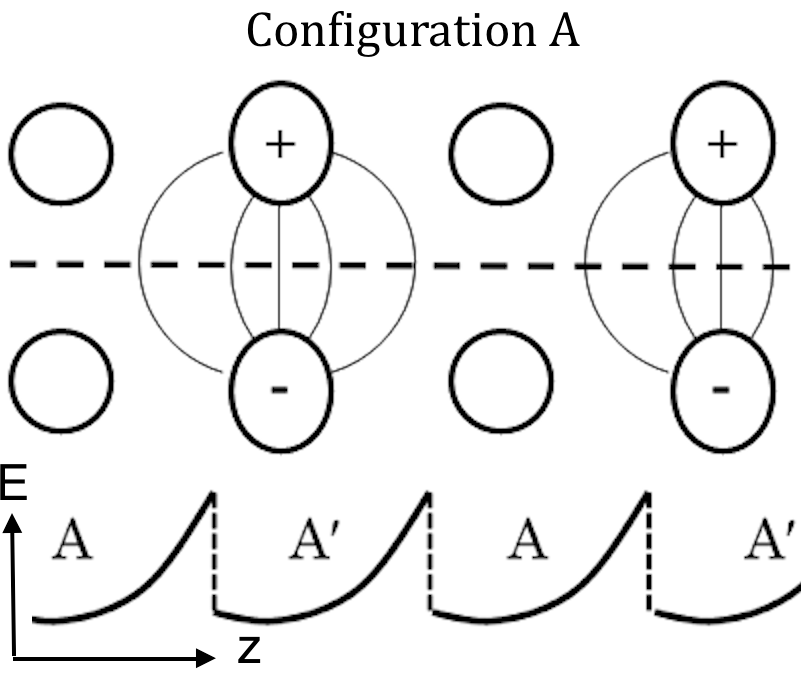
\includegraphics[width=8cm]{chargecartoon.png}%
\caption[Voltages, E-fields, and on-axis Energy]{\label{fig:decelcartoon}
Voltages, electric fields, and on-axis potential energy in a conventional pin decelerator~\cite{Bethlem1999}. 
Pin rotation indicated by representation as slight ellipses rather than circles. Electric fields density corresponds to the potential experienced by molecules. 
The horizontal dashed line indicates the central axis of the device, and the potential energy of the target or synchronous molecule as it transits this axis is shown below the pin pairs. 
A' indicates the translation (and rotation) of the drawn configuration of fields and voltages to the next pin pair(s). 
Vertical dashed lines indicate change in potential energy of a molecule during a switching event between configurations.
}
\end{figure}

Diagrams such as that shown in Fig.~\ref{fig:decelcartoon} are useful in understanding the operation of the device.
Molecules approach a region of strong electric field, exchanging kinetic energy for internal potential energy in the case of those whose quantum state features a positive Stark shift, the only ones capable of being manipulated by such a device.
At some point, the strong electric fields are turned off, and a different region of strong electric field is turned on further along the beam-line.
If the strong fields are turned off before the synchronous molecule reaches the strongest fields, i.e. partway up the hill, phase stability is obtained, because a molecule that is ahead of the synchronous one will therefore exchange a greater quantity of kinetic energy for potential energy by climbing farther up the hill before the turn-off event.
This molecule thus experiences a force restoring it to the location of the synchronous molecule.
Of course if a molecule is too far ahead, it may pass all the way through the region of highest field prior to the turn-off event. Such a molecule is no longer phase stable and will travel farther and farther from the synchronous molecule.
Thus there is a tradeoff between the deceleration capability of the device and the volume of its phase stable region.

\begin{figure}[t!]
\centering
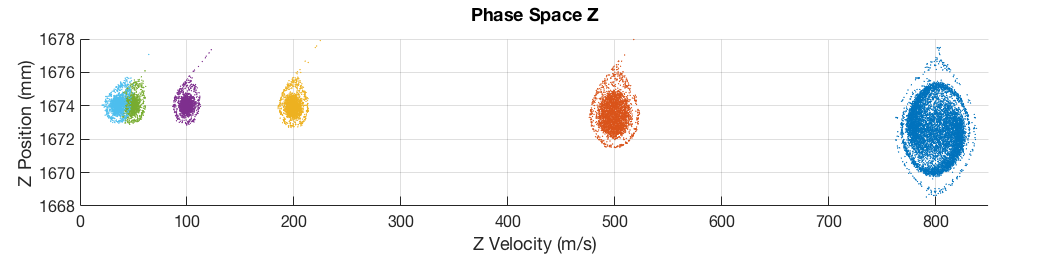
\includegraphics[width=\linewidth]{Slowing/phaseangles.png}%
\caption[Phase Space for Different Final Velocities]{\label{fig:variousphaseangles}
Longitudinal phase space plots of a Stark decelerator with varying final velocity. From left to right, $v_f=33, 50, 100, 200, 500, 800$~m/s. Note how the size of the populated area reduces as the final speed is reduced.  This is a direct reflection of how closely the synchronous molecule approaches the charged pin-pair, which in turn controls how far ahead a non-synchronous molecule may be while still experiencing a restoring force. Note also how the size reduces much more significantly between $800-500-200$~m/s then for any of the other speed reductions. This is described further in the main text. 
}
\end{figure}

This can be seen more directly from simulations of its behavior, such as in Fig.~\ref{fig:variousphaseangles}. The area of the region populated by molecules reduces as the deceleration is increased.
However, the change in area seems to plateau and then stop, somewhere between $200-500$~m/s since all velocities below $200$~m/s show nearly the same area.
This can be attributed to the fact that all of these low speeds require nearly the same energy to be removed per stage of the decelerator, since the total energy removed can be calculated by the potential energy difference:
\begin{equation}
\Delta\text{PE}=\frac{1}{2}m_\text{OH}\left(v_i^2-v_f^2\right).
\end{equation}
Once $v_f << v_i$, $\Delta\text{PE}$ no longer various strongly with $v_f$:
\begin{equation}
\label{slowphasevary}
\Delta\text{PE}\sim\frac{1}{2}m_\text{OH}v_i^2\left(1-\left(\frac{v_f}{v_i}\right)^2\right).
\end{equation}

An important corollary of this idea relates to the parameterization typically used for specifying decelerator operation.
Since the devices are periodic, it is convenient to parametrize the longitudinal coordinate with an angle, called the phase angle, and chosen to vary by $180^\circ$ between one pin-pair in the next, so that a single voltage configuration applied to the backbone repeats itself after $360^\circ$.
This parametrization also allows us to work independently from the choice of pin size and pin spacings for a given device.
A decelerator is often operated so that a synchronous molecule with a given speed would always experience a turn-off event at the same phase angle $\phi$, which then allows the operation of the device to be specified by only that angle.
It follows from Eq.~\ref{slowphasevary} however that very slight changes in $\phi$ can lead to dramatic changes in the final velocity of the synchronous molecule.
In earlier iterations of the code used for programming the switching sequence of our decelerators, it was necessary to specify the phase angle down to the thousandth of a degree in order to get the desired final speed within a few meters per second, which in turn required carefully hand-exploring the function mapping phase angles to final speeds.
This is discussed further in an appendix ??.

It is also worth discussing some other features of the longitudinal phase space plots shown in Fig.~\ref{fig:variousphaseangles}. 
Almost all final speeds show a bullseye type pattern, with a halo of outer particles surrounding an inner core.
This is discussed extensively in~\cite{VanDeMeerakker2006}, and relates to the inefficiencies in the device that are the subject of the next section.
However, there is additional structure evident within the inner core, especially for the molecular packet with $800$~m/s final velocity.
These molecules have not had their speed modified significantly by the simulated device, in which case the activity of the device is better described as ``bunching'' the molecules than ``slowing'' them.
In the experiment, these bunched molecules would travel together with a large population of unaddressed molecules with initial longitudinal velocity and position unsynchronized with the timing of the device.
These unaddressed molecules are nonetheless transversely focused, and in some cases with better efficiency than target molecules, and so constitute a rather large background signal relative to the molecules of interest.
The reason these unaddressed molecules are not evident in this simulation is that the simulation only initializes molecules that are likely to be addressed, for reasons of runtime.

This in turn relates to the substructure evident in the inner core of the bunched molecules in Fig.~\ref{fig:variousphaseangles}.
This substructure is an artifact of incomplete phase space filling in the simulation, i.e. if the right molecules had been included in the initialization, the inner core would be more uniformly filled out and not feature any swirling.
It is useful to keep an eye out for such artifacts as a way of monitoring whether the initialization assumptions of a simulation is valid. 
This swirling is not necessarily only an artifact however, and can in fact be relevant in the experiment as well.
In~\cite{Parazzoli2009}, the rotating nature of the inner core in phase space is intentionally understood and exploited for minimizing the velocity spread of a beam exiting a decelerator.

\section{Alternative Geometries and Configurations}

Alongside the history of achievements enabled by Stark deceleration runs a parallel ongoing saga surrounding their efficient operation. 
Many important steps have been made, not only in understanding the flaws of the conventional pulsed decelerator~\cite{VanDeMeerakker2006,Sawyer2008a}, but also in addressing them through the use of overtones~\cite{VanDeMeerakker2005a,Scharfenberg2009}, undertones~\cite{Zhang2016}, or even mixed phase angles~\cite{Parazzoli2009,Hou2013}. 
Even with these advances, the outstanding inefficiencies of the pulsed decelerator, particularly with regard to transverse phase stability, have motivated alternative geometries such as interspersed quadrupole focusing~\cite{Sawyer2008a} and traveling wave deceleration~\cite{Osterwalder2010,VandenBerg2014,Fabrikant2014}. 
Although traveling wave deceleration takes a strong step in the right direction toward truly efficient operation, it comes with costs in system complexity and high voltage engineering. 
These costs can be partially addressed by the use of combination pulsed and traveling wave devices~\cite{Quintero-Perez2013}, or even using traveling wave geometry with pulsed electronics~\cite{Hou2016,Shyur2017}. 
Others continue to pursue brand new geometries aiming to enhance transverse acceptance without abandoning more reliable pulsed electronics~\cite{Wang2016}. 

\subsection{Flaws in Conventional Deceleration}

I begin here by describing more precisely these flaws in the conventional pulsed decelerator.
It is useful to distinguish between two primary categories of performance breakdown:
\begin{enumerate}
\item Breakdown associated with the discontinuous nature of the geometry.
\item Breakdown associated with the nature of the phase stable region.
\end{enumerate}
The first breakdown mechanism follows directly from the geometry of the conventional pulsed decelerator. Focusing only occurs in a given transverse direction every other pin pair. So if the speed of the beam is decreased enough, there is clearly a point at which molecules will be adversely effected.
The same issue exists for the longitudinal direction. Switching events are required for molecules to experience restoring force in the longitudinal direction. When molecules do not encounter pin pairs with enough frequency, molecules again are adversely affected.
Discontinuity breakdowns are thus further classified by their transverse and longitudinal manifestations- over-focusing and reflection loss- discussed further in~\cite{Sawyer2008a}.
These breakdowns can in general be described by a lower bound on the velocity of the beam:
\begin{equation}
v_z >> Lf_\text{osc} \label{breakdownequation},
\end{equation}
where $z$ indicates the propagation direction, $L$ indicates the distance between successive pairs of pins, and $f_\text{osc}$ is the oscillation frequency of the molecules about the synchronous molecule.
This latter parameter is not strictly well defined across the entire ensemble, but accepts a range of possible values according to the anharmonicity of the restoring force experienced by molecules with different deviations from the synchronous molecule.
For typical operating conditions, $f\sim 1-2\text{ kHz}$.

\begin{figure}[t!]
\centering
\includegraphics[width=\linewidth]{Slowing/many-bunching-plots.png}%
\caption[Phase Space for S\,=\,1, S\,=\,3, and S\,=\,311]{\label{fig:bunchingphasespace311}
Longitudinal phase space plots after several types of bunching for several decelerator lengths. Column-wise, operation is in S\,=\,1, S\,=\,3, and a hybrid of these that I term S\,=\,311. Indicated percentages are comparable by rows, but suffer from a pernicious simulation artifact. Some molecules are included which actually pass through decelerator pins. The effect adversely influences the comparative survival numbers, but not the observed projection of phase space onto the longitudinal direction.
}
\end{figure}

This anharmonicity is at the core of the second kind of breakdown in performance of the pulsed decelerator, a breakdown which results in unwanted decreases in the flux of the device even without any of the issues associated with low final speeds.
In fact, the effect is already clearly manifested for devices operated in bunching mode without any slowing, refer to Fig.~\ref{fig:bunchingphasespace311} for the following discussion.
One way to understand these flaws is to think in terms of an unwanted coupling between transverse and longitudinal modes~\cite{VanDeMeerakker2006}.
In words, molecules are best focused transversely on their closest approach to the charged pin pair, and therefore molecules which deviate significantly from the synchronous molecule in the longitudinal direction experience the best transverse focusing.
It follows that the two directions of motion are strongly coupled to one another, and any full description of their equations of motion will not be separable.
It also follows that molecules would survive better at greater distance from the synchronous molecule in longitudinal phase space, which agrees nicely with the observed sparsity close to the center of the left four plots in Fig.~\ref{fig:bunchingphasespace311}.
The dead band and outer ring are best explained in terms of parametric amplification phenomena~\cite{VanDeMeerakker2006}.

One way to address this is to allow the molecules to pass all the way through a charged pin pair, and only switch the fields after they climb a second hill.
This is known as overtone operation~\cite{VanDeMeerakker2005a}, where the term stems from the fact that even without intending it, the standard operating mode supports overtone operation for molecules that happen to begin at triple the intended speed.
Or one may intentionally reduce the switching frequency by a factor of three, typically indicated by the overtone parameter S as S\,=\,3 operation, in which case standard operation may be referred to as S\,=\,1.
This gives rise to the much more homogeneous set of phase space plots in the center column of Fig.~\ref{fig:bunchingphasespace311}.
Despite improved homogeneity, the plots are thinner than those for S\,=\,1 by a factor of $\sqrt{3}$, which stems from the fact that molecules experience restoring force in the longitudinal direction with one third frequency. 
They can therefore deviate from the synchronous molecule by only a third as much kinetic energy as before, or $1/\sqrt{3}$ less deviation in velocity.
An even more important drawback of S\,=\,3 operation is that only a third as much energy may be removed per unit distance.

It is also possible to use a hybrid approach that we term S\,=\,311.
In this operating mode, one allows the synchronous molecule to climb all the way over a hill only every third time.
It should be noted that $S\,=\,31$ operation, where the synchronous molecule climbs all the way over a hill every other time, is not as useful because this molecule would only experience extra focusing in one of the transverse directions.
This mode has the advantage of sacrificing less deceleration capability, since it is $60\%$ as effective as S\,=\,311 since $3/5$ of all possible hills are climbed, but also addressing some of the coupling issues.
As can be seen in the last column of Fig.~\ref{fig:bunchingphasespace311}, the sparsity closest to the synchronous molecule at the center of the phase space is addressed, although a parametric amplification dead band still persists.
Unfortunately this mode also features an increased sensitivity to low speeds.
Typically, S\,=\,1 operation stops performing due to low speed breakdown below $50$~m/s, and S\,=\,3 below $150$~m/s.
The cutoff has not been studied thoroughly for S\,=\,311, but a hybrid alternative exists, which is to use S\,=\,311 for the bulk of the deceleration except when the speed drops below $150$~m/s, at which point one returns to S\,=\,1 for a brief enough time that the transverse-longitudinal coupling does not lead to excessive loss.
In practice, this has yielded factor of $2-3$ improvements in the number of molecules which may be slowed or trapped in our experiment.
I spent some time seeking to determine the source of the discrepancy between this improvement and the smaller one predicted by the simulations leading to Fig.~\ref{fig:bunchingphasespace311}, and only years later caught a simulation bug relating to molecules with large transverse deviation ghosting their way through decelerator pins without being removed.

\subsection{Alternative Geometries}

Perhaps the most important class of alternative geometries for deceleration are those that are continuous in nature. 
These include both Stark~\cite{Osterwalder2010} and Zeeman~\cite{Narevicius2008} varieties, and in principle provide a complete solution to breakdowns associated with the discontinuous nature of pulsed geometries, although in practice they face various low-speed challenges of their own.

The Stark devices, also known as traveling wave decelerators, feature cylindrical symmetry and use sinusoidal voltages to generate a macroscopic moving trap which can be translated or decelerated, and even brought to rest, at least provided high voltage amplifiers with bandwidth down to DC operation.
The most common and as far as I can tell the only geometry used thus far, in three or four different groups, is that described in~\cite{Osterwalder2010} with $0.8$~mm diameter wires bent into $4$~mm inner diameter rings, and connected up to eight different backbone electrodes.
Their total phase space acceptance, at least for lower decelerations, is an incredible improvement over S\,=\,1 operation, skip ahead to Fig.~\ref{fig:efftrap} and compare S\,=\,1 to $TW$ in panel (b).

There also exist a host of proposals for alternative pulsed geometries, including this one with interspersed quadrupole focusing stages~\cite{Sawyer2008a}, this one with charged wires for improved transverse behavior~\cite{Wang2016}, and even a magnetic device with interspersed hexapole stages for use with NH molecules~\cite{Plomp2019}. The first two may become less important thanks to the results discussed in the next section. Perhaps the earliest attempted device appears to have used actual parallel plates and relied on their fringing fields for focusing~\cite{Golub1967}, as would have been necessary given the speed of available switches at the time.

I would be remiss if I did not introduce a few new geometry proposals of my own, as have my predecessors~\citep[Sec.~5.5]{SawyerThesis2010}, \citep[Sec.~7.3]{HudsonThesis2006}.
The first, motivated by the trapping configuration discussed further in Sec.~\ref{sec:pintrap}, is to add magnetic focusing to each decelerator pin.
The idea would be to use dual domain magnetic pins to superimpose 2D magnetic quadrupole focusing fields on top of the entire decelerator.
This has the potential for vey substantial benefit as far as transverse performance is concerned, see the vastly enhanced phase space volume shown in Fig.~\ref{magneticdecel.png}.
Unfortunately, this design would suffer from very significant spin flip losses due to the presence of orthogonal magnetic and electric fields.
Molecules would likely shuffle back and forth between \f3 and \fm3, with any favorable focusing effect completely washed out.
A molecule besides OH with a $J=\frac{1}{2}$ ground state (CH, CF, NO~\cite{VanDeMeerakker2006thesis, weibel1998hexapole}) could be much more likely to benefit from this scheme, since these molecules do not feature the electric field enhanced spin-flip behavior derived for $J=\frac{3}{2}$ OH molecules in Sec.~\ref{sec:der}.
I do not provide a formal proof of this, but the path to the proof is that the spin-flip enhancement requires the Zeeman effect to have cubic order with orthogonal fields.
This cubic order relates to the order of perturbation theory required to get a coupling between the \f3 and the \fm3 states, since their $m$ number differs by $3$. 
In a $J=\frac{1}{2}$ molecule, the $m$ number differs by only one, so that the Zeeman effect would remain linear.
I have also confirmed this by numerically diagonalizing sample Hamiltonians with $J=\frac{1}{2}$.

\figdave{magneticdecel.png}{A Magnetic Pin Stark Decelerator}{By adding magnetic domains to the pins of a conventional Stark decelerator, dramatic gains in transverse performance can be obtained. Here a factor of three is found, even with dramatically under-filled simulated phase space is evident by the swirling structure in the longitudinal phase space.}{\linewidth}

And secondly, it is my distinct pleasure to introduce the double-pin decelerator, a brand new design, specially featured thus far only here in this thesis.
The double pin decelerator uses a pair of pins everywhere that a normal decelerator would feature only a single pin.
Instead of overlapping each other, pairs of double pins point directly towards each other, with a well-controlled tip-to-tip spacing.
Manufacturing of the device is therefore somewhat more sensitive, although the regions of the pins which need to be highly polished are reduced, and the tips of pins are by far the best polished portions when tumble polishing is performed.
The key idea behind the use of pairs of pins is to try to obtain a focusing effect in both transverse directions each stage.
It could also be thought of as a pulsed ring decelerator with each ring split in half to enable more significant deceleration forces by building up field between the two halves.
The idea is to make use of two different field distributions obtained by charging the device up in different ways.
One is like in conventional deceleration, when a pair of double pins are oppositely charged; the other occurs when the pair are charged to the same voltage, but preceding and following pairs of double pins are charged to an opposite voltage.
The field distribution resulting in the latter case would ideally resemble that in a ring decelerator. 
This concept is also very relevant for the conventional geometry, and discussed at length in the next Section, Sec.~\ref{sec:afd}.

\figdave{doublepin.png}{The Double Pin Decelerator}{(a) Geometry view showing arrangement of the double pins. (b-c) $x-y$ planar cuts through a pair of double pins showing the magnitude of the electric field, color axis kV/cm, contours every $10$~kV/cm. Pins have $3$~mm diameter, $1.5$~mm adjacent spacing, $2$~mm point to point spacing, and $2$~mm stage to stage spacing. (b) The slowing hill with the pair oppositely charged. $40\%$ less height than conventional deceleration and some defocusing. (c) Now with the pair charged to the same voltage and un-shown preceding and following pairs of double pins charged to the opposite voltage.}{\linewidth}

The field distributions generated by the device are shown in Fig.~\ref{doublepin.png}.
The transverse focusing effect when pairs of pairs are charged to the same voltage is a big win compared with conventional operation, and even a modest win over a conventional decelerator with alternative field distributions run in VSF mode, described further in Sec.~\ref{sec:afd}.
However it features a good bit of asymmetry, and has much better focusing for molecules that deviate along $\pm\vec{x}\pm\vec{y}$ compared with $\pm\vec{x}$ or $\pm\vec{y}$, see Fig.~\ref{doublepin.png}c.
It also has $40\%$ less slowing power than a conventional decelerator, and some defocusing in one direction while slowing.
These drawbacks could be partially addressed by shaping the double pins more like half of a ring, but this would drastically reduce manufacturability.

\subsection{Alternative Field Distributions}\label{sec:afd}

As far as the conventional geometry is concerned, a much more effective route to improved performance is to mix alternate field distributions into the deceleration scheme that feature strong restoring force in the transverse directions, refer to Fig.~\ref{fig:chargecartoon}.
%This restoring force averages into the effective moving trap, leading to the dramatic improvements over S\,=\,1 shown in Fig.~\ref{fig:efftrap}. 
In the conventional S\,=\,1 operating mode~\cite{VanDeMeerakker2012}, molecules approach a charged pin-pair, climbing a hill in potential energy. 
The hill is abruptly switched off partway up the hill, allowing molecules to have phase stability as discussed above.
But it follows that molecules spend a significant portion of their flight passing between grounded pins.
Conventionally, pins are always charged in bipolar pairs, in which case few field lines run toward the grounded pin-pairs, and those that do actually create a slight defocusing effect.
This defocusing is not obvious in Fig.~\ref{fig:chargecartoon} because those plots are generated by slicing so as to include the decelerator axis but also make a $45^\circ$ angle with all pin axes.
This choice has the distinct advantage of allowing the plain to intersect all pairs of pins, making it much more clear where they are.
However, the defocusing effect is significantly stronger in the plane orthogonal to the grounded pin pairs, and is thus obscured.

\begin{figure}[t!]
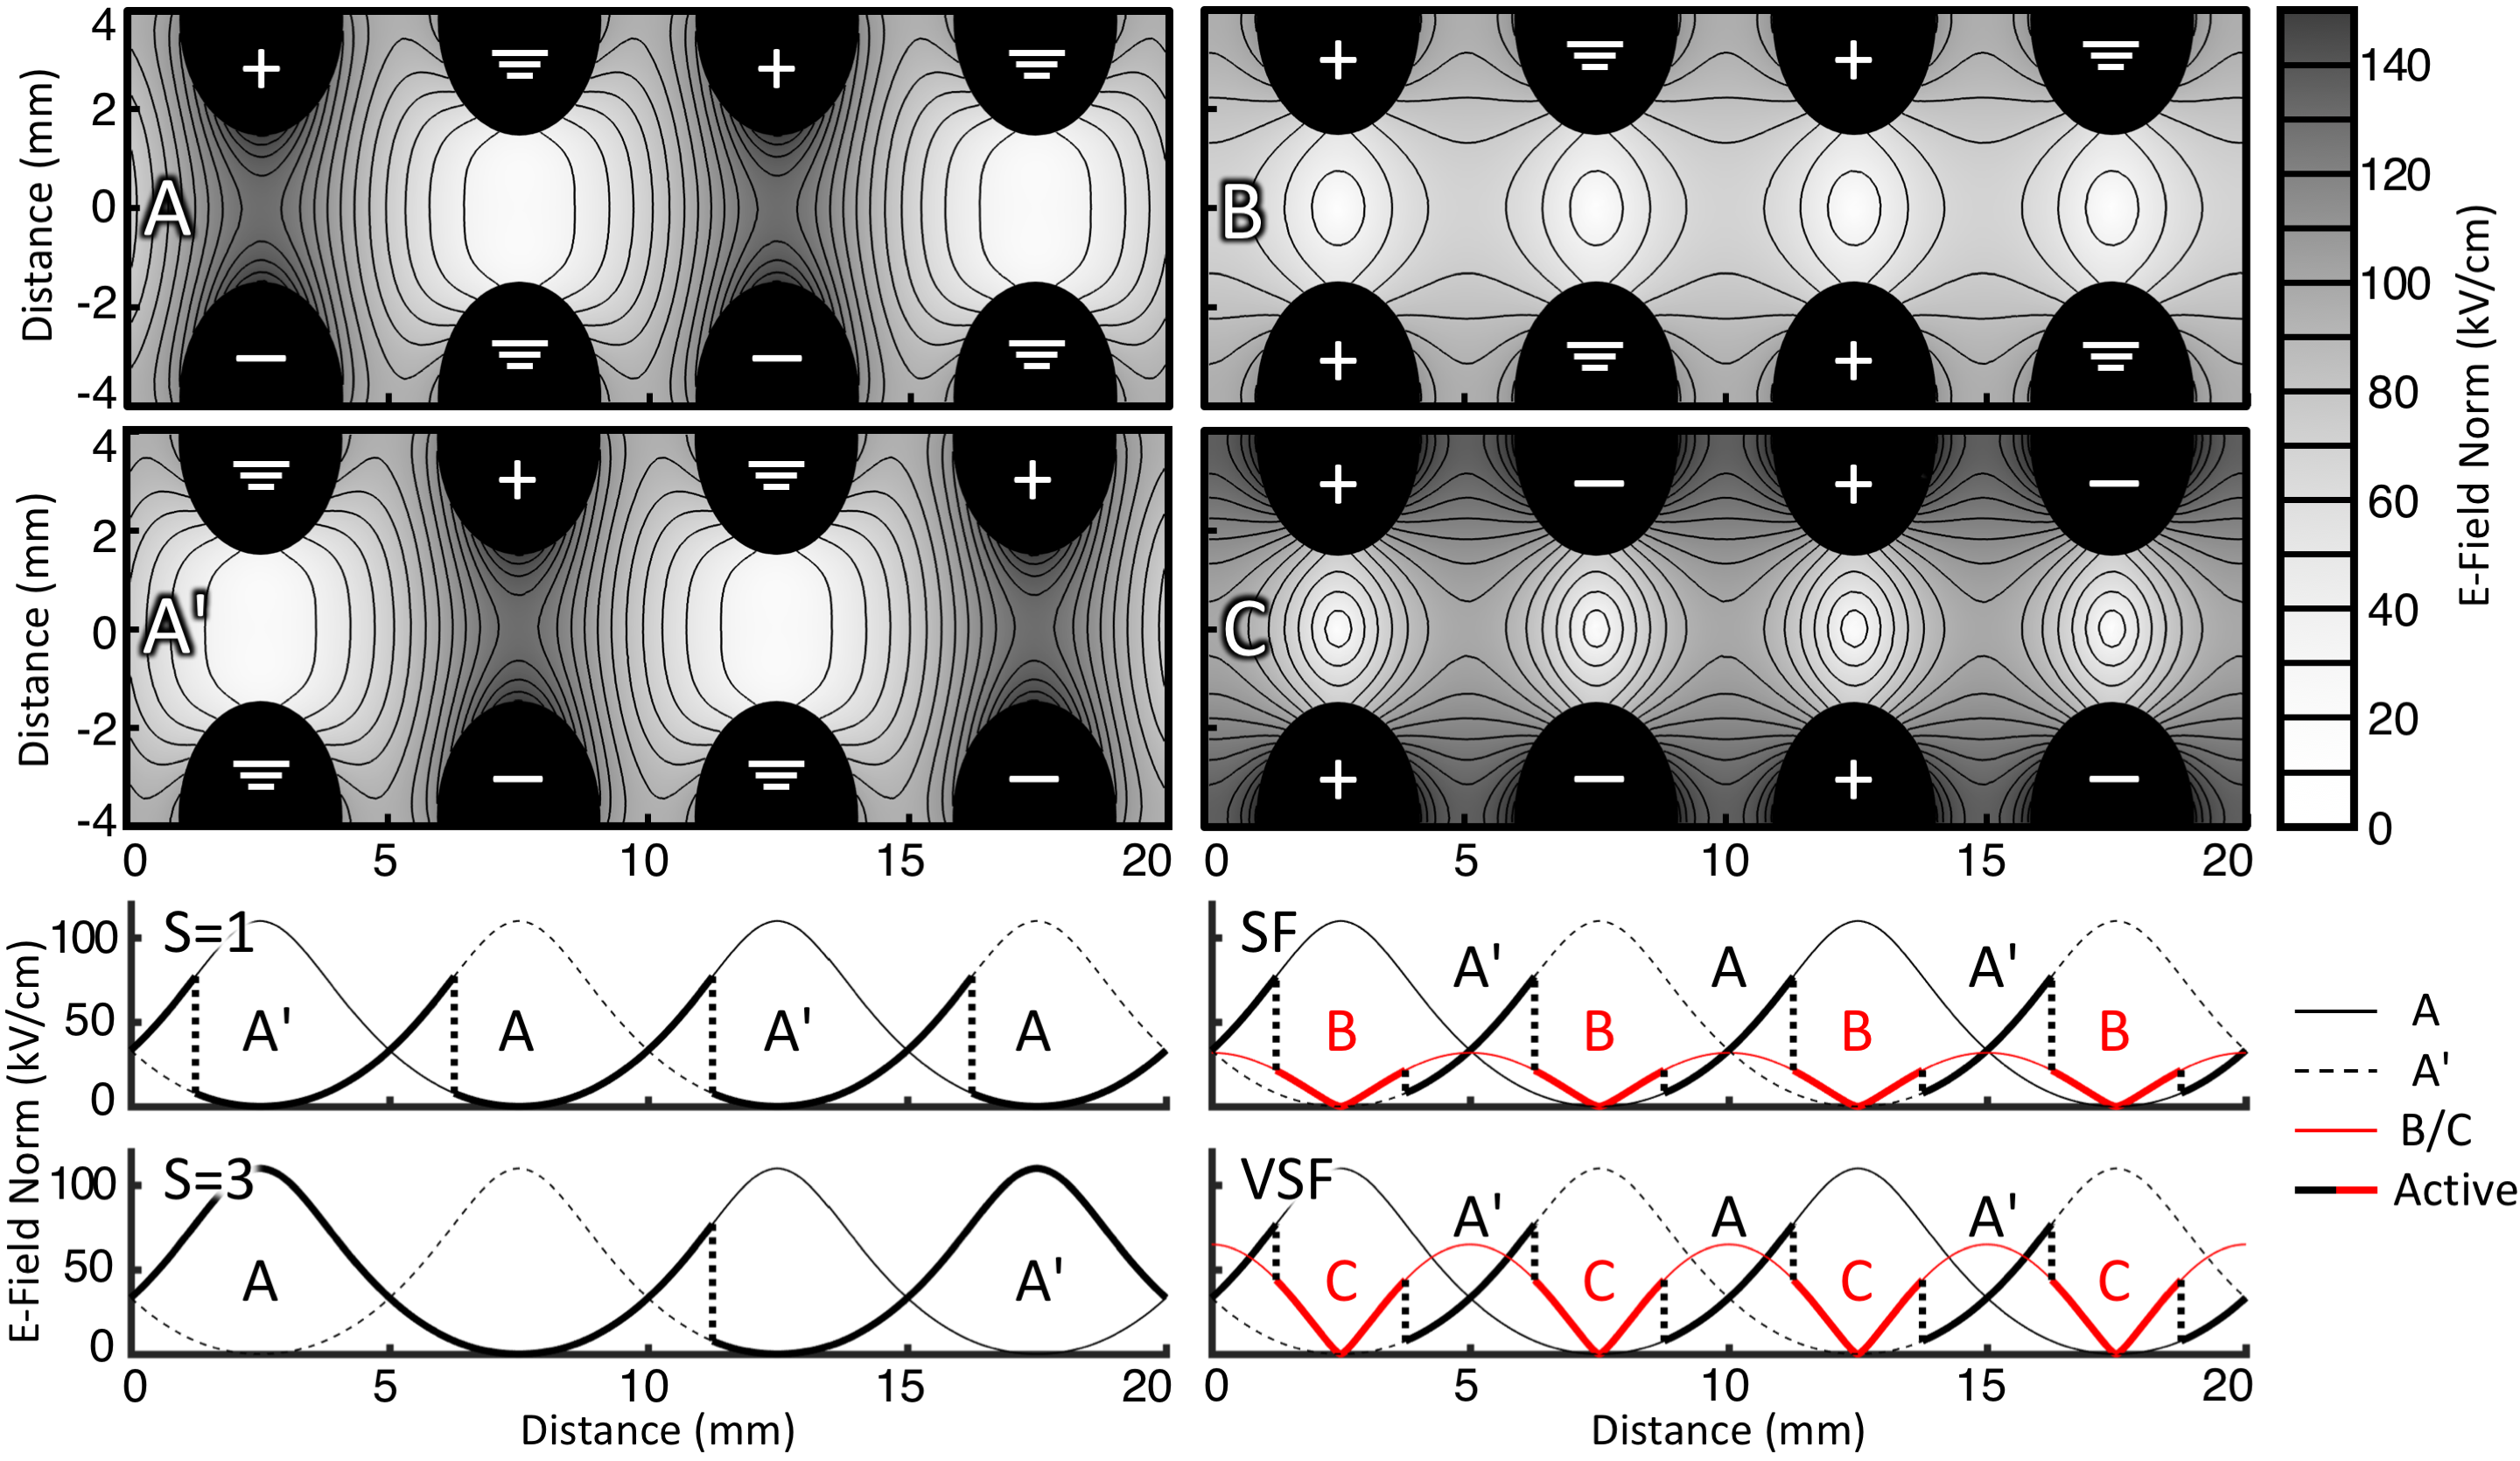
\includegraphics[width=\linewidth]{Slowing/pinpairformal.png}%
\caption[Definition and Explanation of Alternate Field Distributions]{\label{fig:chargecartoon}
Alternate field distributions which can be used alongside the conventional one for greatly enhanced performance. Configurations B and C feature strong transverse focusing in the regions where molecules would normally pass between grounded pin pairs. On-axis energy diagrams are shown for several modes of operation incorporating these alternate configurations, with primes indicating translation to the next pin pair. In addition to S\,=\,1 mode and its S\,=\,3 overtone~\cite{VanDeMeerakker2005a}, a strong focusing (SF) and a very strong focusing (VSF) mode are introduced.
}
\end{figure}


Useful alternate configurations can be created by applying voltage in a way that is not balanced between adjacent pin pairs. 
Once an imbalance exists, by charging up both pins in a pair to the same non-zero voltage, by only charging one pin in a pair, or even by unbalancing the decelerator power supplies\footnote{It was once noted that unbalancing the power supplies led to improved performance on a conventional pulsed Stark decelerator. S. Hoekstra, private communication.}, the field lines will run between pin-pairs. 
Near the grounded pin-pair, these field lines create a focusing 2D quadrupole structure, much like this one used intentionally for trapping and controlling spin-flip losses~\cite{Reens2017}. 
By implementing these configurations when the synchronous molecule is flying between the grounded pin pair, but retaining the use of the conventional configuration for hill climbing, the longitudinal behavior of the device is unaffected while the transverse behavior is vastly improved.
Regarding spin-flip losses, use of these configurations is cause for concern, but not significant as far as early modeling is concerned. This is discussed further in Sec.~\ref{sec:spinflipdecel}.
Utilizing the field distribution that results when both pins in a pair are brought to the same voltage gives rise to a new strongly focusing operation mode (SF), and utilizing the distribution where the adjacent pin pair is also brought to the voltage opposite the first gives a very strongly focusing mode (VSF). 

It is also possible to obtain some of these effects without the need for rods being charged to three different voltages, by making use of the field distribution generated by turning on only a single pin, a somewhat focused mode (F).
This is especially significant for being realizable immediately on existing devices with no new electronics, and offers 4-fold gains at trappable speeds, see Fig.~\ref{fig:speedvary}.
Operation in F mode requires alternating between the two choices of which pin in a pair should be charged and which should be grounded, in order to balance out the asymmetry of the resulting field distributions.
The field distributions and on axis energy diagrams indicating when they are to be used are also shown in Fig.~\ref{fig:speedvary}.

\begin{figure}[t!]
\centering
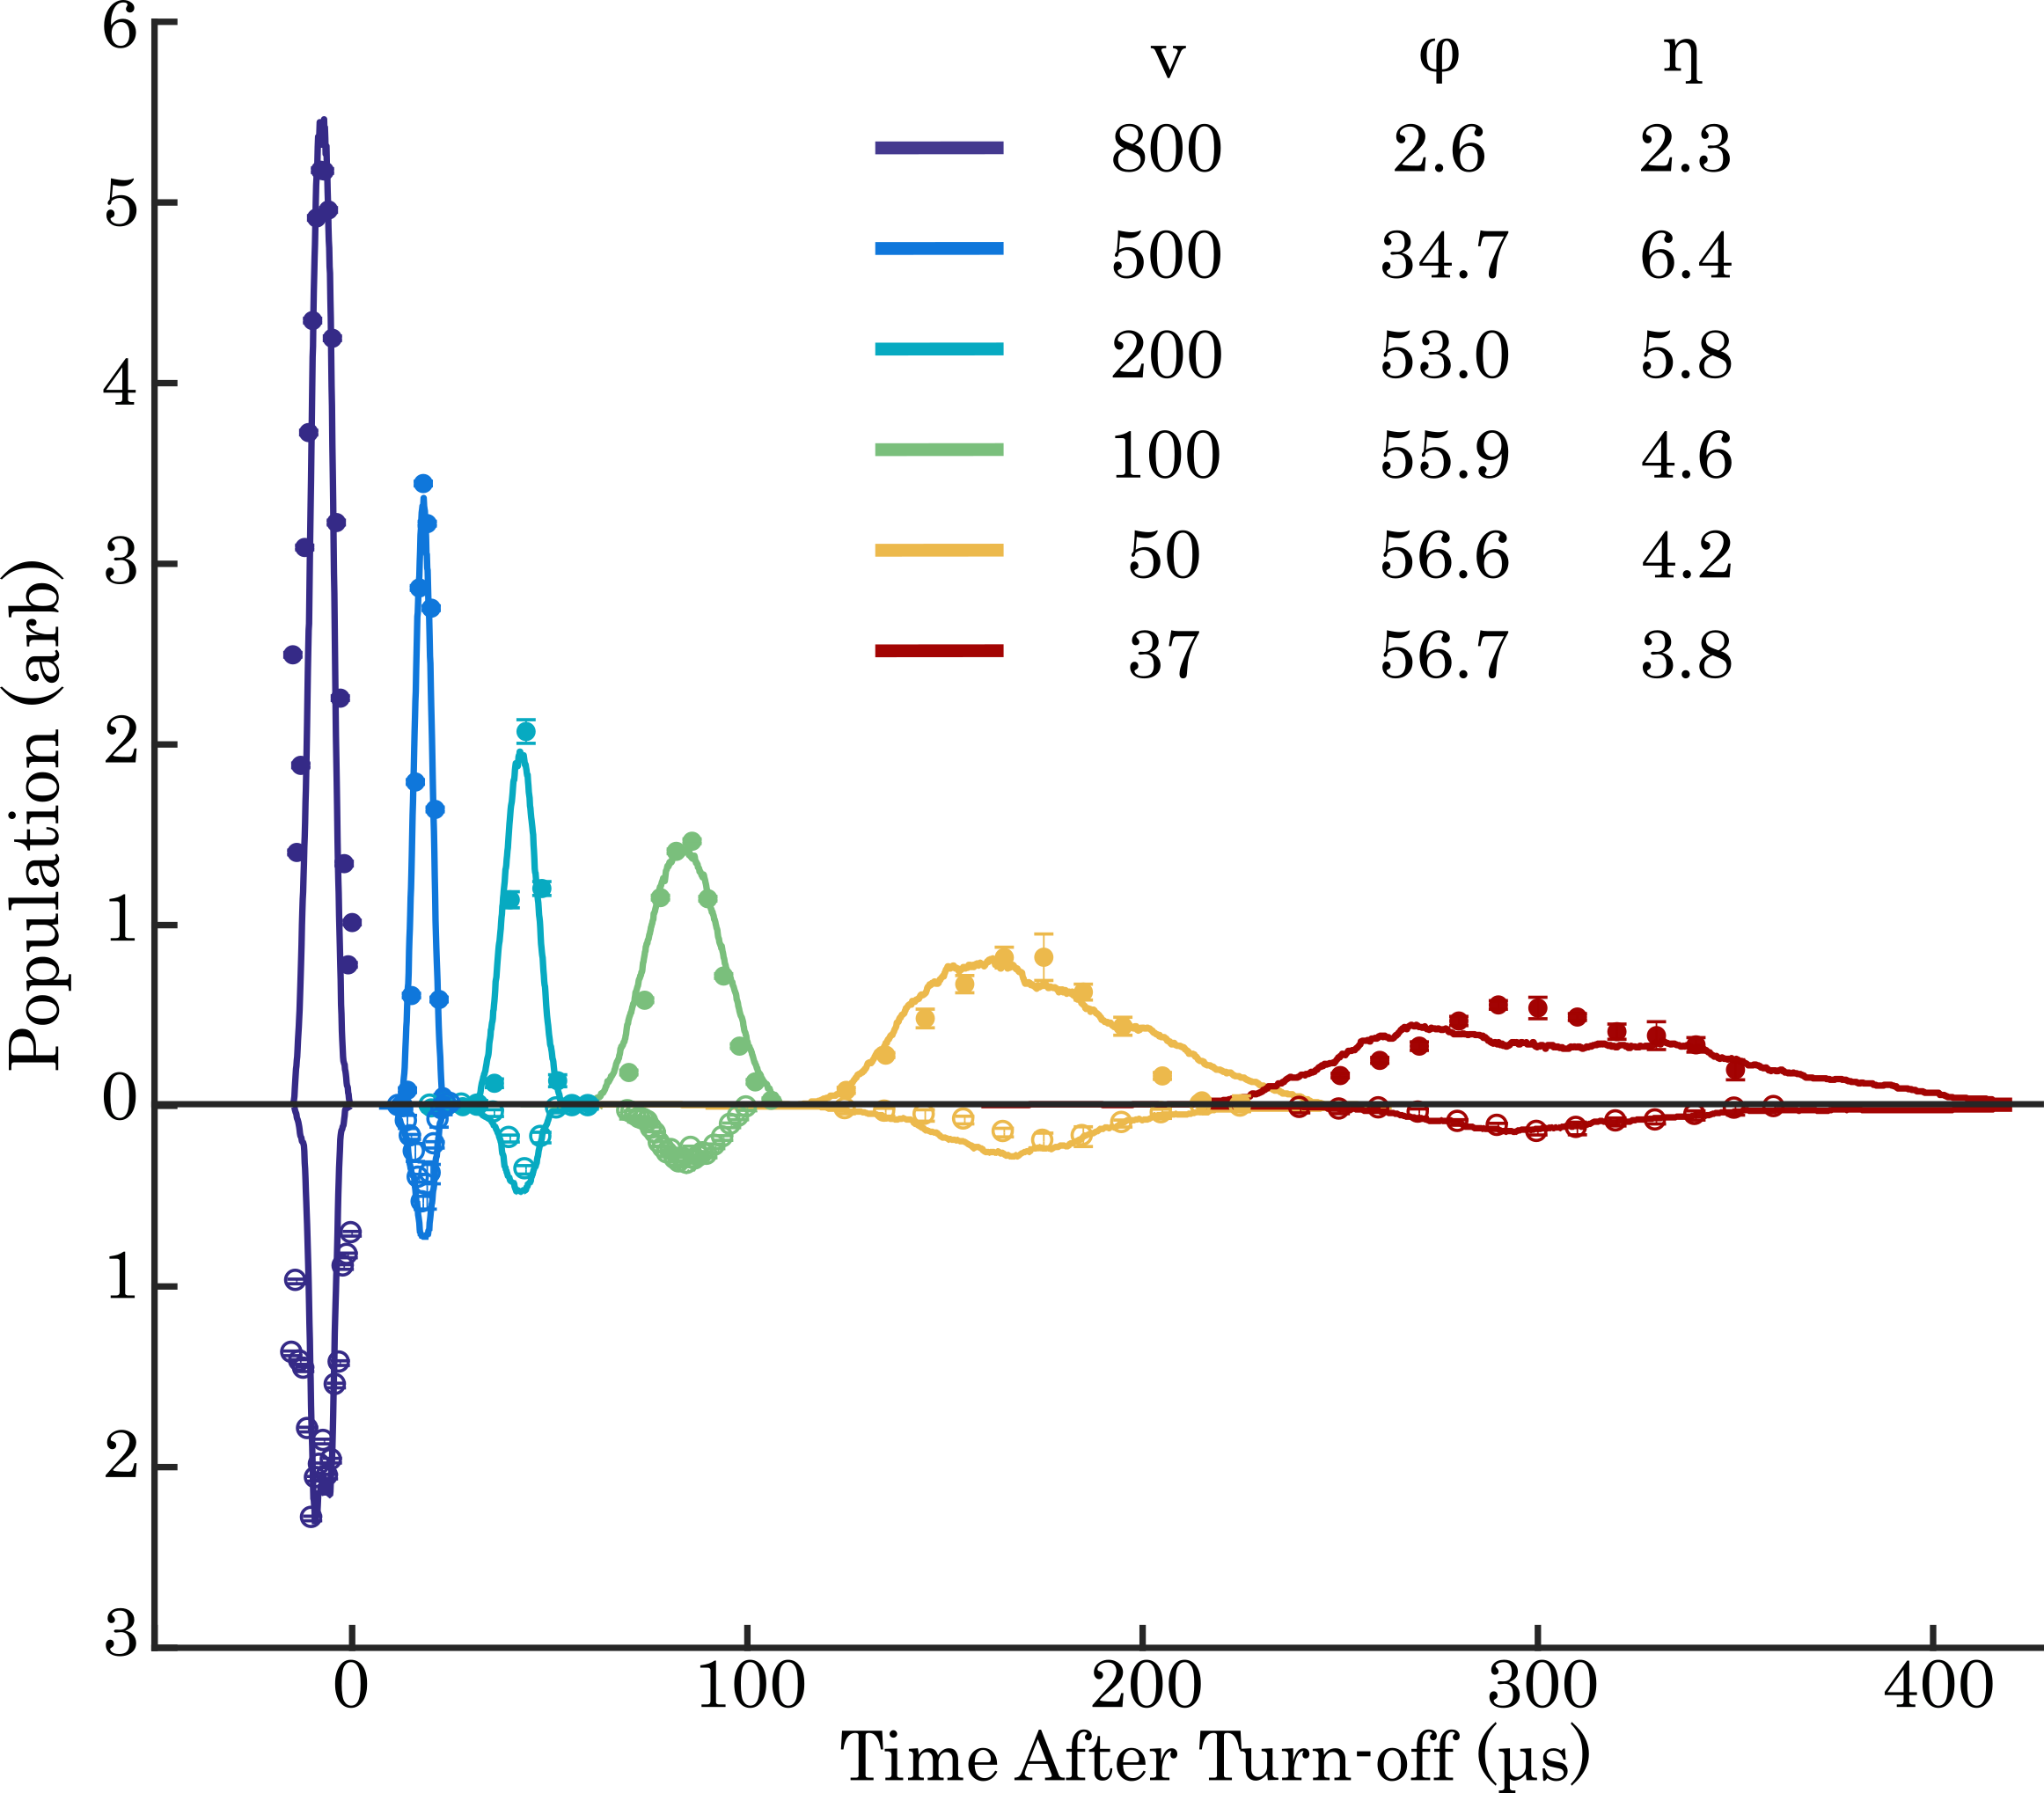
\includegraphics[width=7.5cm]{speedvary.png}\hspace{4mm}
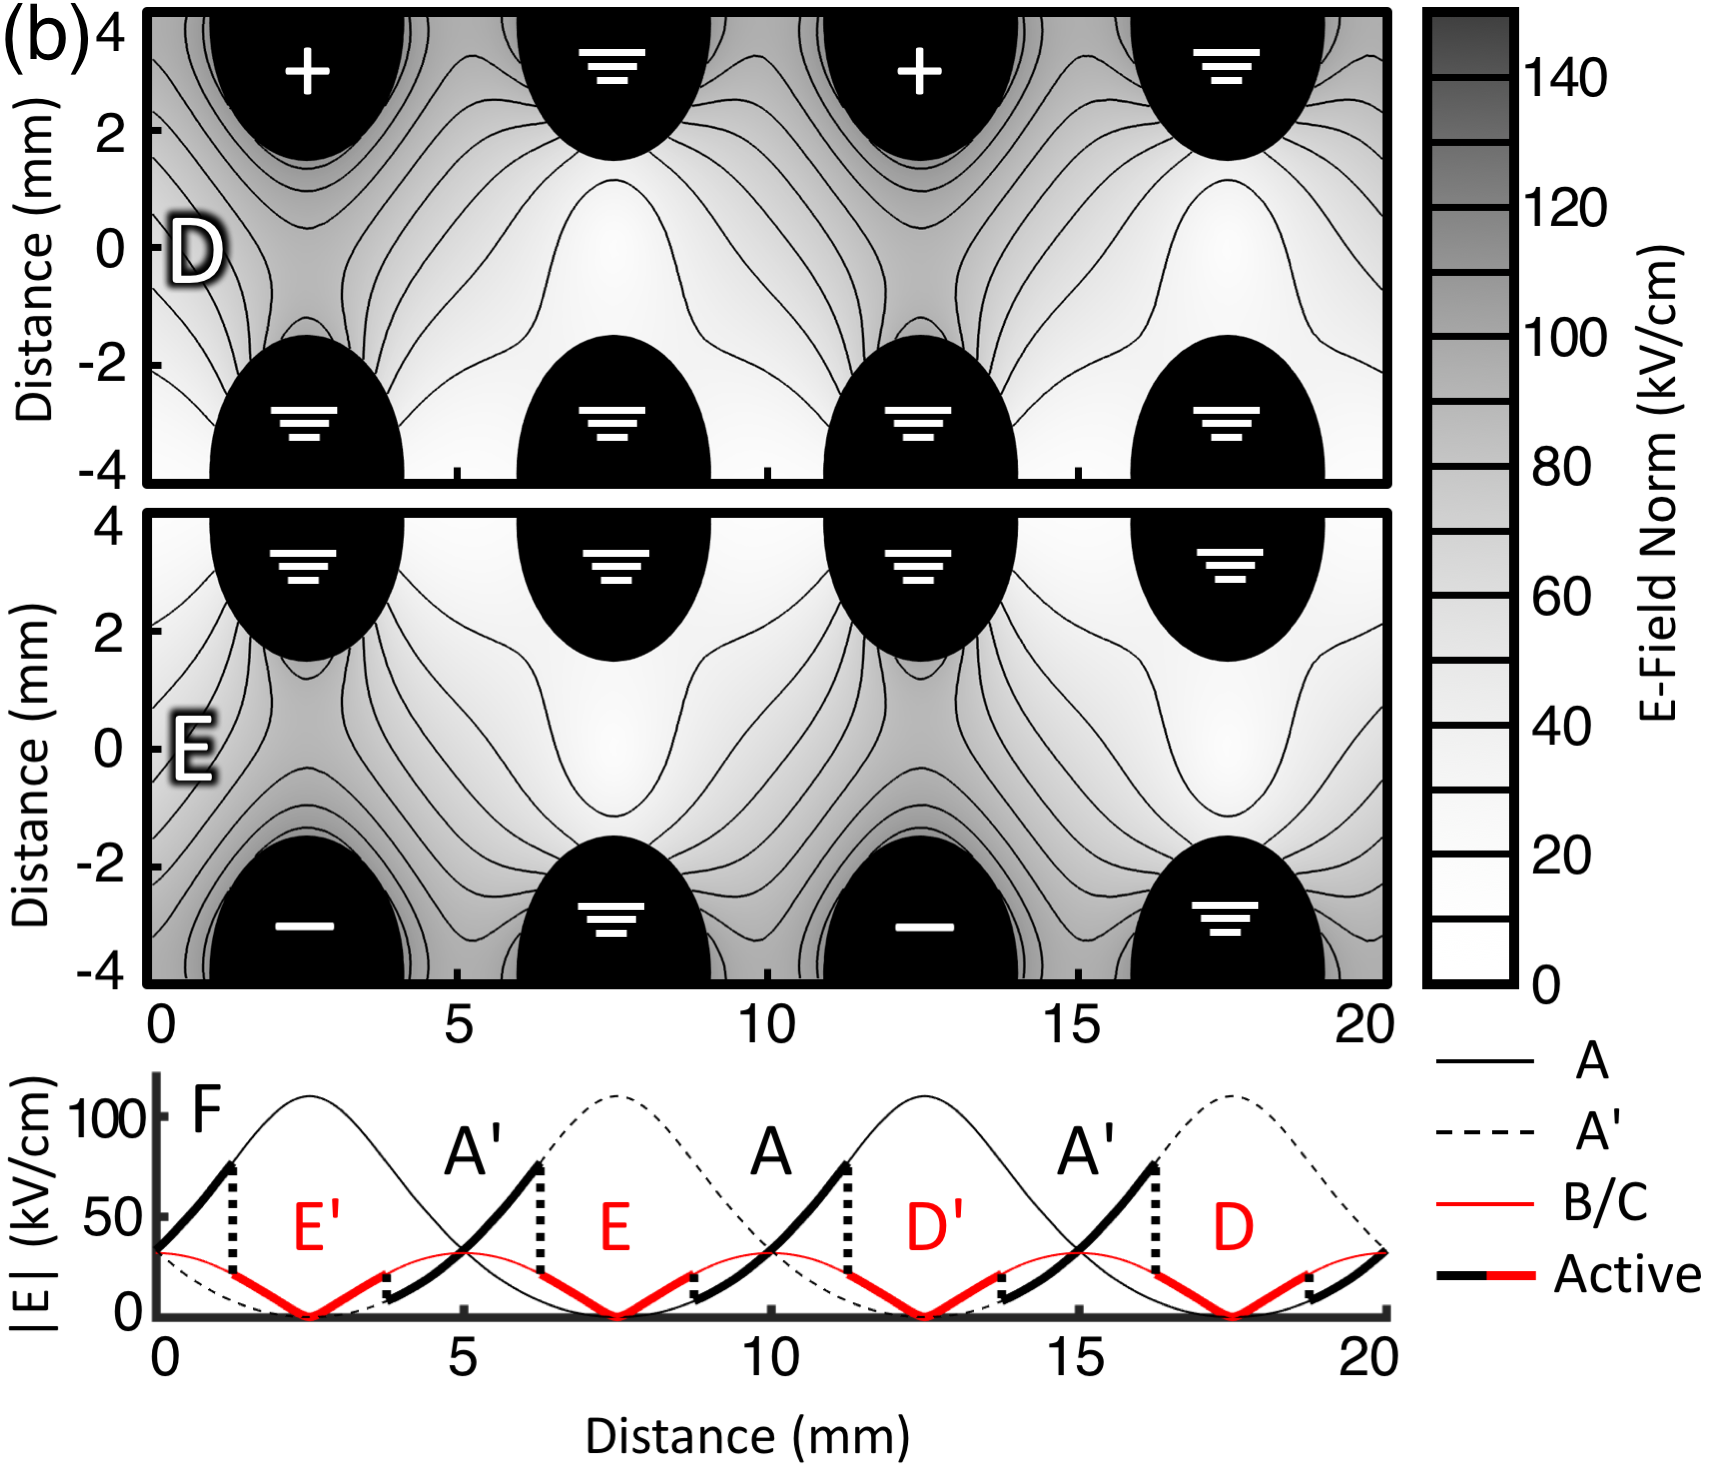
\includegraphics[width=7.5cm]{pinpairF.png}%
\caption[S\,=\,1 and F Mode Comparison]{\label{fig:speedvary}
(a) Experimental Data Comparing S\,=\,1 and F mode. Fourfold or greater improvements are found across many final velocities. F mode traces are shown with positive sign, and S\,=\,1 with negative for visual comparison. Simulations are performed and reported as solid lines; good agreement is obtained.
(b) Diagrams like in Fig.~\ref{fig:chargecartoon}, but for $F$ mode. At bottom, the potential energy of the alternate distributions (red) are still those for configuration B of Fig.~\ref{fig:chargecartoon} for reasons of simplicity, but the labels are as appropriate for $F$ mode.
}
\end{figure}

An important feature of the required time sequence of field distributions is that in switching from $A$ to $E$ configuration, a single rod may be switched off and the other left on, so that relative to S\,=\,1 operation, the total number of switching events for each rod is unchanged.
This is important because it means that the total energy dissipation in the high voltage system is unchanged, so that no improvements to the thermal dissipation capability of existing high voltage systems are necessary.
This discussion ignores the fact that turning off a single rod without the other also turning off actually requires more energy ($\sim 20\%$) than turning both off at the same time~\ref{capmatsection}. 
In practice however, extra capacitance in the decelerator will primarily influence the thermal load on the external limiting resistors, which are usually not chosen within $20\%$ of failure, and can have a cooling fan added easily.
For the high voltage FETs themselves, cooling power can be a more sensitive parameter, but with the limiting resistors in place, most of their heat load actually comes from discharging their internal parasitic drain source capacitance, which therefore depends only on the number of switching events and not the capacitance of the load.


\subsection{The Effective Moving Trap}
In order to quantitatively analyze these and other operation modes, we can work in the non-inertial moving frame of the molecules, where any feasible mode generates an effective trapping potential with deceleration included as a fictitious force. 
%One of the key motivations for improvement of the conventional pulsed decelerator operation are its well-known failings as far as phase-space stability is concerned. These have been described in terms of transverse-longitudinal couplings~\cite{VanDeMeerakker2006}, small separatrix area at high phase angles~\cite{Hudson2004}, or reflection at low velocities~\cite{Sawyer2008a}. 
This approach is usually reserved for continuous deceleration schemes~\cite{Osterwalder2010,Narevicius2008}, but is equally valid for pulsed schemes provided their velocity satisfies Eq.~\ref{breakdownequation}. 
The effective trap for on-axis molecules in the longitudinal direction has been discussed at length~\cite{Bethlem2000,Hudson2004}, but computation of the full 3D effective trap has not been reported previously.
The 3D effective trap is evaluated numerically for various operation modes to obtain the equipotential surfaces in Fig.~\ref{fig:efftrap}d.
It is found that for S\,=\,1, the effective trap has holes. 
Molecules moving away from the trap center along the $x$ and $y$ axes experience almost no restoring force at all. 
This can be considered the underlying reason for the transverse-longitudinal coupling problem discussed above. 
Such couplings are in some contexts useful for maintaining ergodicity in a trapping geometry~\cite{Surkov1996}, but with one dimension featuring a very low energy barrier, they lead to loss.

\begin{figure}[t!]
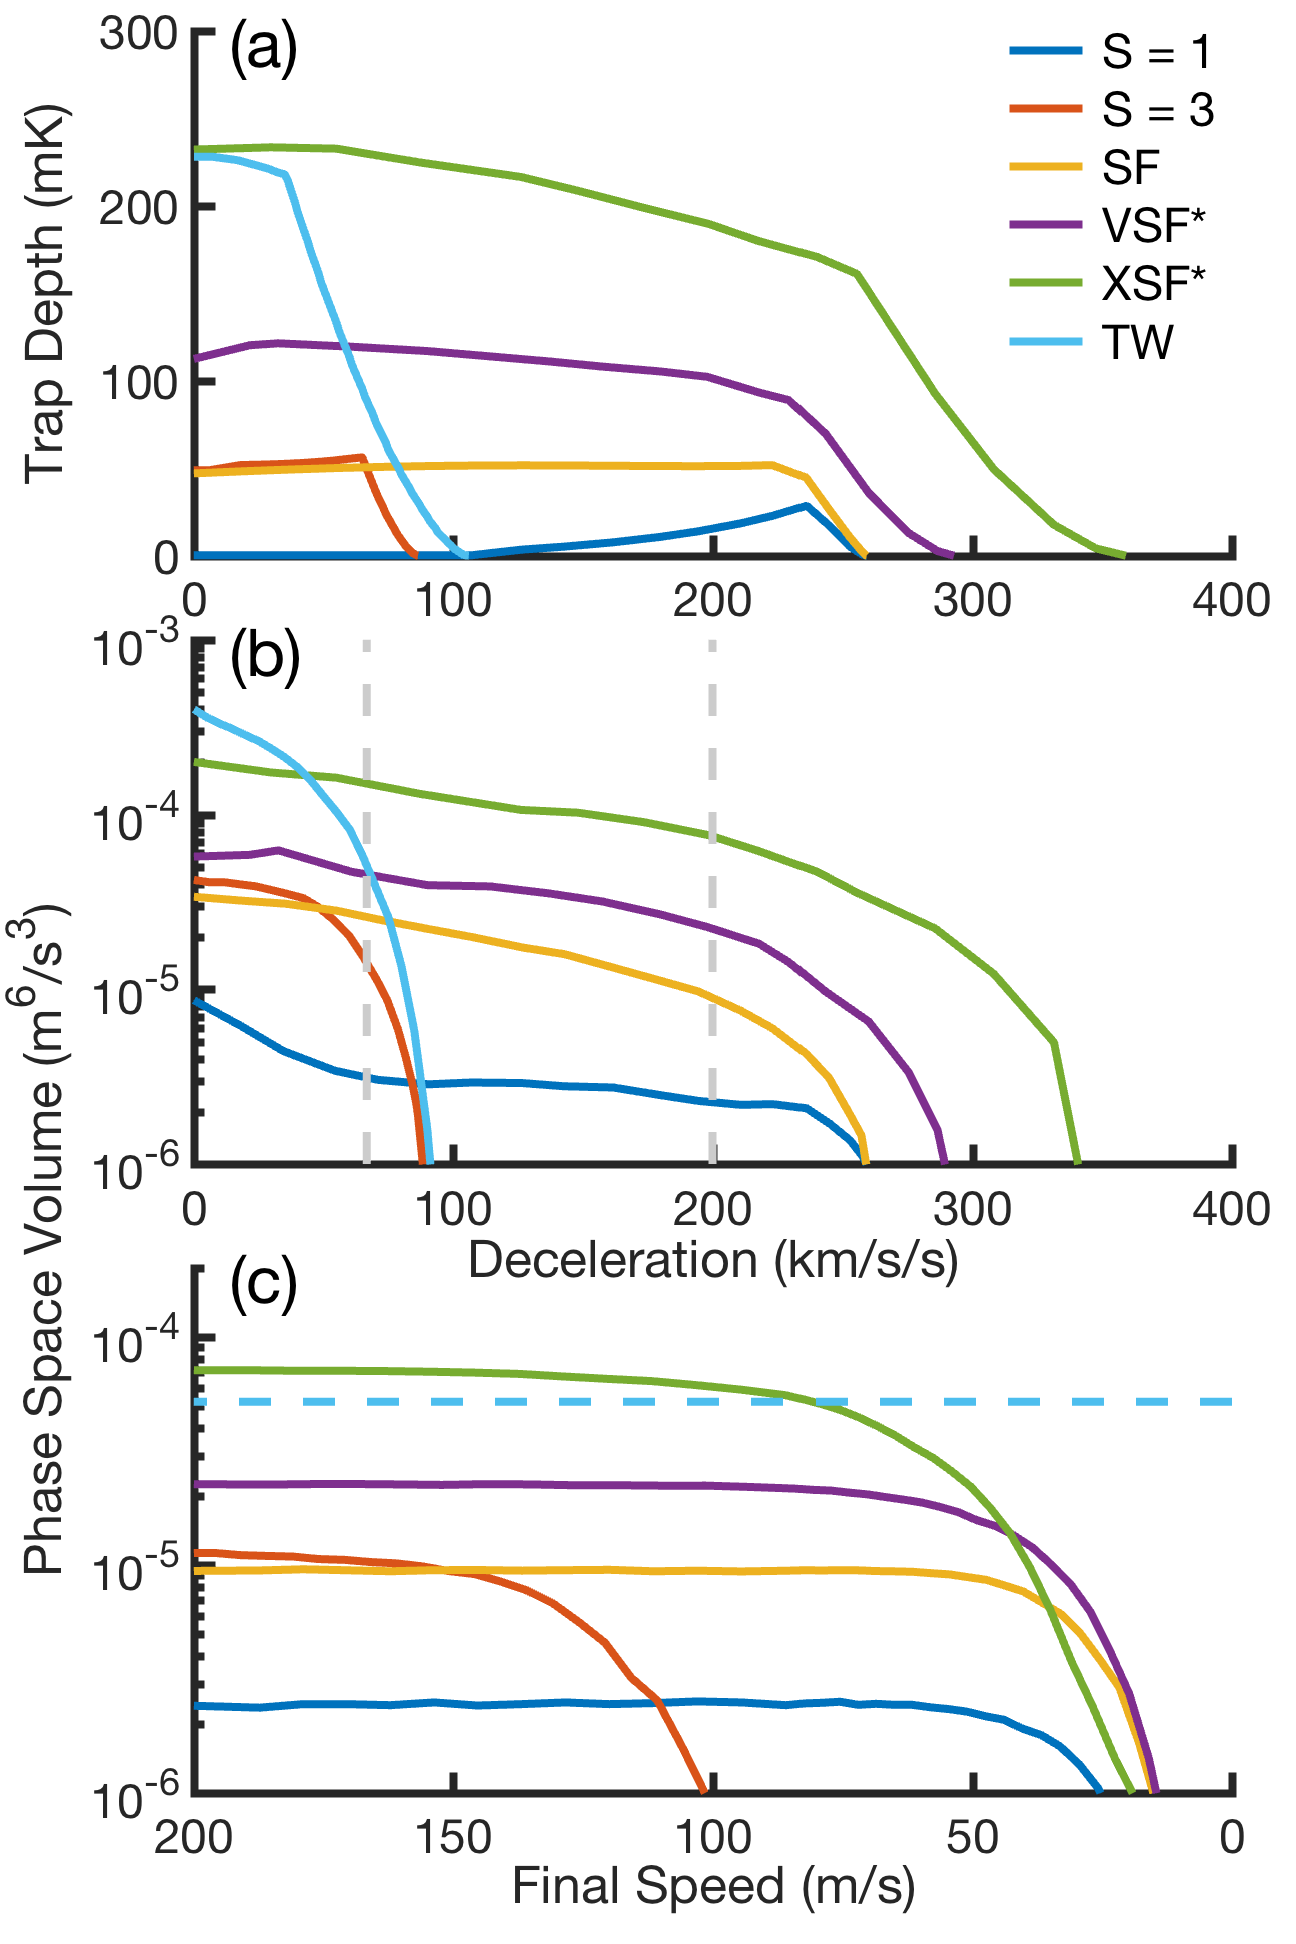
\includegraphics[width=\linewidth]{Slowing/full-three-panel.png}%
\caption[Traveling Potential Well Characteristics for different Modes]{\label{fig:efftrap}
Characterizing the moving trap under different modes of operation. In addition to the conventional S\,=\,1 and S\,=\,3 modes, newly defined strong focusing (SF), very strong focusing (VSF), and focusing (F) modes are shown. Traveling wave (TW) deceleration is also compared, assuming $10$ kV peak to peak, to our knowledge the largest voltage used to successfully decelerate to rest with a TW device. In panel~(a) the trap depth at the lowest point of escape is shown as a function of deceleration for different operating modes. The stars on SF and VSF indicate $\phi_2$ tuning, see the text. In panel~(b) the initial phase space volume remaining within these effective traps after a $3$~ms hold time is shown, and in panel~(c) a full decelerator simulation is performed as a function of final velocities, with hold time fixed also at $3$~ms and deceleration fixed as indicated by the gray dashed lines in panel~(b). For TW a full simulation is not performed, since low speed losses are less significant, but the dashed line shows the value corresponding to 67 km/s/s in panel~(b). In panel~(d) equipotentials give a feeling for the effective trap as a whole, which is helpful for visualizing the derivation of the minimum trap depth in panel~(a). The effective traps shown correspond to $\phi=45^\circ$, about $180\text{ mK}$. The propagation axis is to the right, and transverse directions are up and diagonally outwards.}
\end{figure}

Motivated by the holes evident in S\,=\,1 mode, a new figure of merit that may be used to compare the performance of various modes of operation is introduced: the minimum depth of their effective moving traps.
Here minimum depth refers to the smallest energy above which a molecule with that energy can find a way out of the trap.
Having a single value to characterize effective traps allows doing so systematically across many modes and across many magnitudes of the applied deceleration, see Fig.~\ref{fig:efftrap}a. Remarkably, F mode offers comparable trap depth improvement to S\,=\,3, but with no sacrifice in deceleration capability. 
The SF and VSF modes make still more dramatic improvements, with the latter even rivaling traveling wave (TW) deceleration~\cite{Osterwalder2010}. 
Note that for SF and VSF, the alternate configurations are not utilized in a symmetric manner about the grounded pin pair as for F. 
Instead, allowing them to be used asymmetrically opens up a new degree of freedom, which is optimized so as to maximize the minimum depth.

It is useful to discuss this tuning a bit further. 
A very similar process was used in~\cite{Zhang2016}, where multiple switching events were employed during a single stage.
The present case is similar in having two different switching events in a stage, one happening at the usual position, call it $\phi_1$, and another, $\phi_2$, happening earlier.
In~\cite{Zhang2016}, extra switching events still only made use of configurations $A$ and $A'$, but enabled greater transverse focusing power and also opened up other opportunities for more specifically tailoring the effective trapping potential.
The same is true in the present case, as far as the increased opportunity for specific tailoring. 
Perhaps the simplest decision is to simply set $\phi_2=-\phi_1$, which has the extra benefit of making no change to the relationship between phase angle and deceleration rate relative to S\,=\,1 operation,  since the molecule doesn't gain or loose any extra energy while in the alternate configuration.
This decision gives good results across a wide range of values of $\phi_1$, but not close to $\phi_1=90^\circ$, where $\phi_2$ becomes nearly identical to $\phi_1$ and the alternate configuration is hardly employed at all.
It is also a poor decision close to $\phi_1=0^\circ$, since in this case $\phi_2$ becomes nearly $180^\circ$ off from $\phi_1$ and the normal configuration is hardly used.
The switch back and forth from the normal configuration is essential to obtaining restoring force in the longitudinal direction, so this would also be a poor choice.
Instead, by tuning the location of $\phi_2$ to optimize the minimum trap depth and not always choosing $\phi_2=-\phi_1$, SF and VSF modes can be more fully leveraged.
This is evident in the phase space plots shown in Fig.~\ref{full5x2phasespace}. 
F mode can be seen to feature greater depth longitudinally than transversely based on the larger projected area of the population, but for SF and VSF the projected area is comparable between the transverse and longitudinal plains.
This is a direct reflection of the fact that $\phi_2$ has been tuned for optimal minimum trap depth, because what happens in this case is that longitudinal depth is exchanged for transverse by increasing the time spent in the transversely focusing direction.

\begin{figure}[t!]
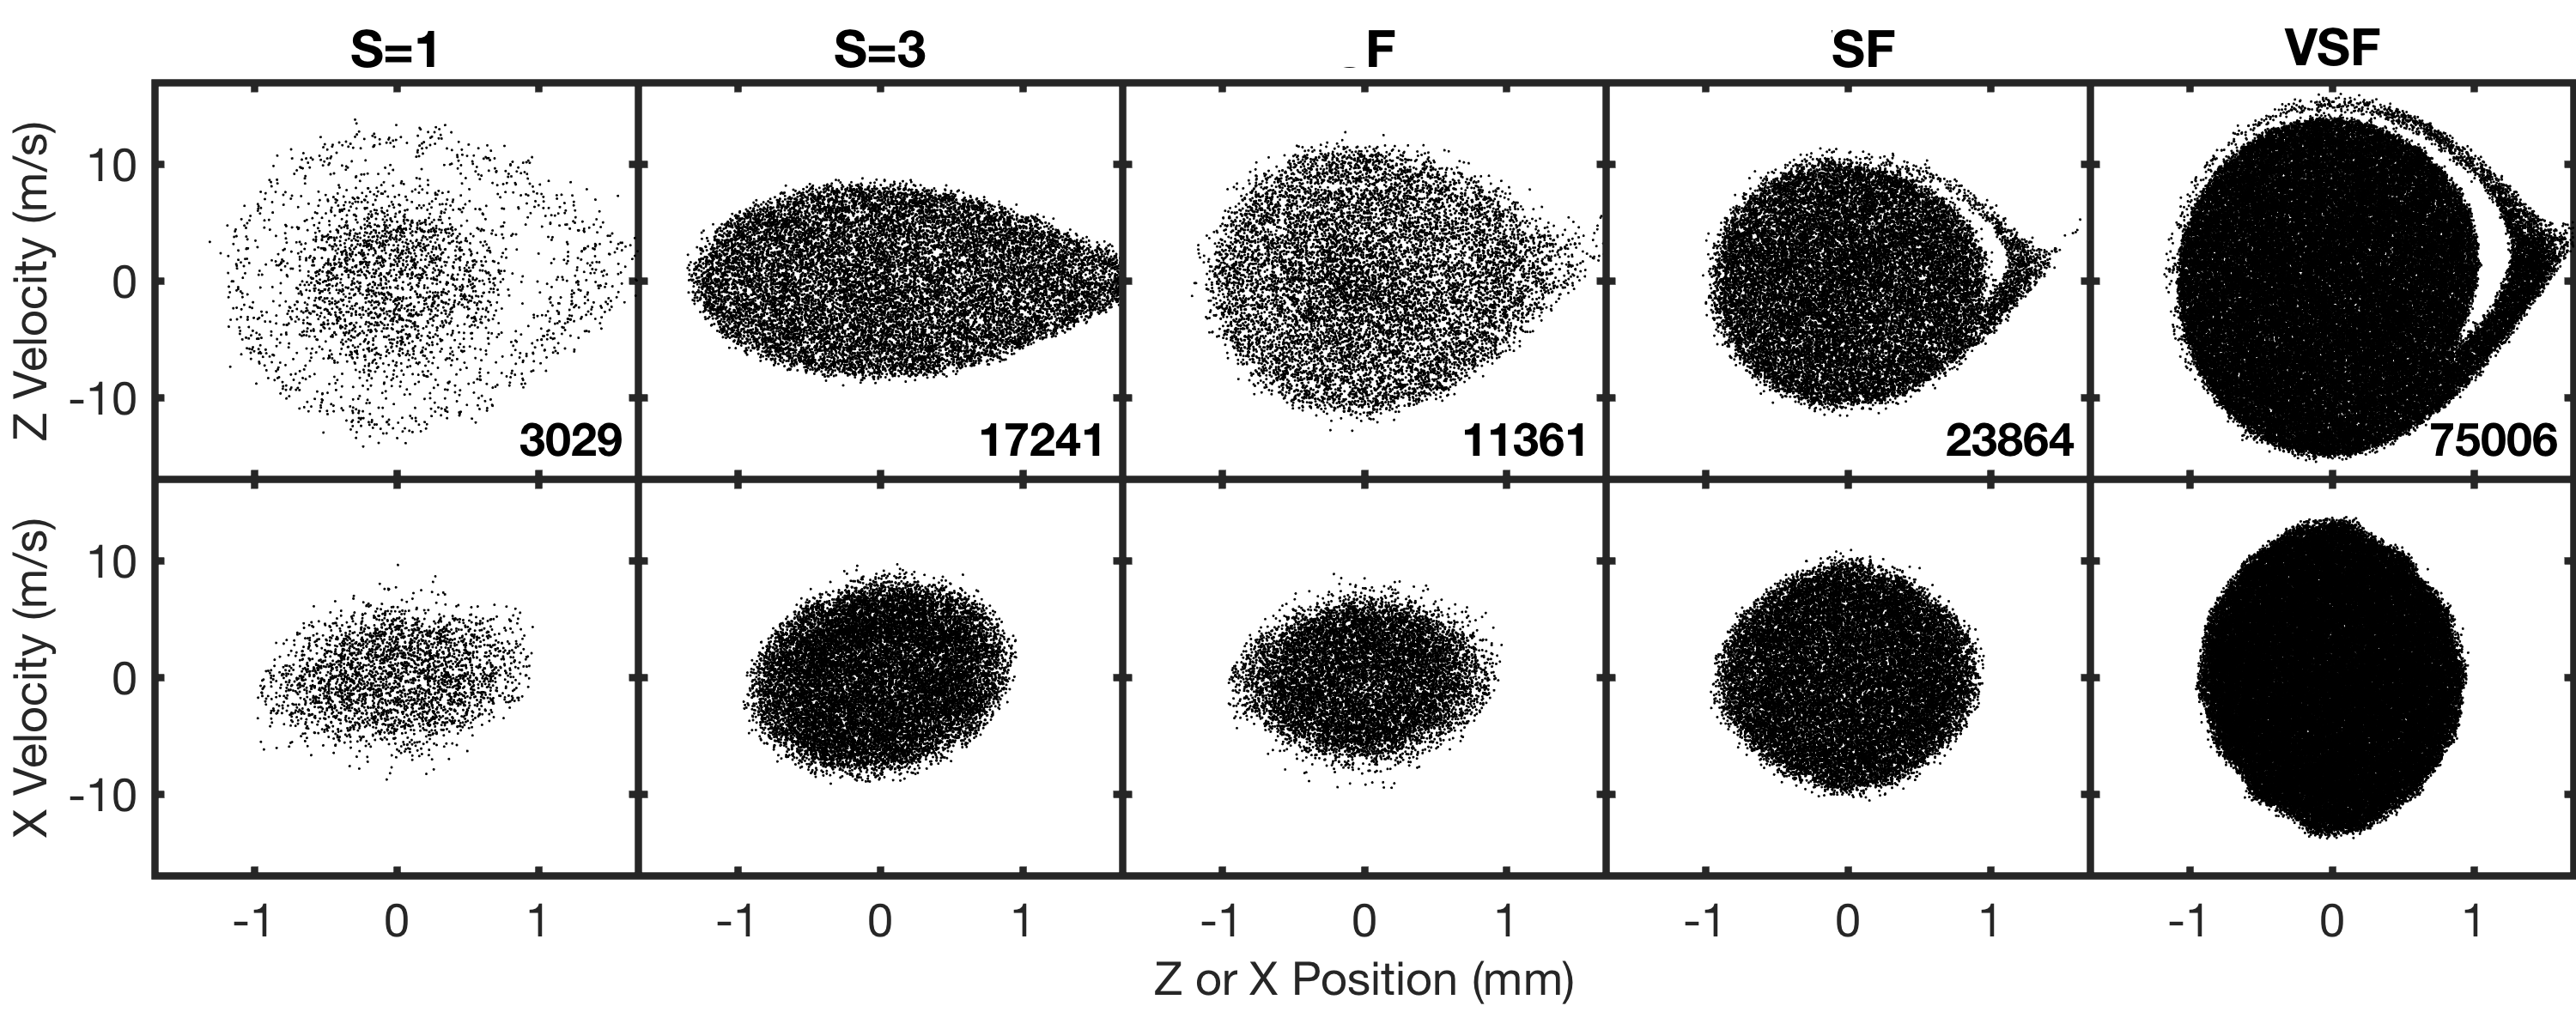
\includegraphics[width=\linewidth]{5x2-PSD-Compare.png}
\caption[Longitudinal Phase Space for different Modes]{\label{full5x2phasespace}
Longitudinal Phase Space Fillings are shown for several operation modes as labeled. 
All modes are initialized with the same uniformly distributed phase space, and the surviving number of molecules is indicated for each pair of panels.
Note dramatic improvements in homogeneity and planar density, without significant broadening to larger velocity classes except for VSF. 
Molecules travel $333$ stages, begin at 900 m/s, and slow at 200 km/s/s (67 km/s/s for S\,=\,3).
}
\end{figure}

We can make further use of the effective trap by directly employing it to simulate the fate of particles confined for $3\text{ ms}$, the duration of a typical deceleration sequence (Fig.~\ref{fig:efftrap}b). 
The results show a very close qualitative match to the trends predicted by the minimum trap depth. 
The most notable exception is found in S\,=\,1 mode at low decelerations, where extremely deep holes dominate the minimum trap depth, but the small effective cross sectional area of the holes still allows molecules to survive in greater number than at higher decelerations where the minimum trap depth actually improves.
As far as the comparison with TW is concerned, it is important to point out that we use the rather small $2\text{ mm}$ pin-pair spacing and $2$x$2\text{ mm}^2$ opening area of our device, while TW devices use $4\text{ mm}$ diameter rings.
If VSF mode were used with a $3$x$3\text{ mm}^2$ device~\cite{Scharfenberg2009} or a $4$x$4\text{ mm}^2$~\cite{VanDeMeerakker2005}, phase space volume would increase significantly, depending approximately on the cube of pin-pair spacing, and thus outperforming TW. 
Deceleration does also reduce linearly with pin-pair spacing, since this influences the number of pins that may be fit next to one another in a given longitudinal distance.

Of course the validity of using the effective trap in this manner depends on the final speed after the deceleration sequence.
This effect can be isolated by also performing a full Monte-Carlo simulation of the various deceleration modes, without use of the effective trap approximation.
By varying only the final speed, and keeping deceleration and run-time exactly fixed by appropriately varying initial speed and decelerator length, we obtain the results shown in Fig.~\ref{fig:efftrap}c, an exact isolation of the low speed effects from other phase space effects.
The asymptotically flat profiles at high enough speeds validate the effective trap picture, as do the quantitative agreement between the asymptotic values and the corresponding points at $200\text{ km/s/s}$ and $67\text{ km/s/s}$ in Fig.~\ref{fig:efftrap}b. 

The beginning of the low-speed breakdown depends on the intended use of the decelerator, and especially how far the molecules will be expected to travel unguided afterwards. 
In Fig.~\ref{fig:efftrap}c, the molecules still confined within a $3\text{ mm}$ diameter circle after $5\text{ mm}$ free flight after the end of the sequence are shown. 
This is a conservative representation of what is required for trap-loading, but for collisional experiments a larger flight distance may be required.
Note how F and SF cut off at even lower speeds than S\,=\,1, but VSF cuts higher. 
This can be attributed to the fact that VSF actually features an increased transverse trap frequency relative to the others, while F and SF improve over S\,=\,1 mostly by plugging holes and not by increasing the trap's depth or frequency.
This restricts the usefulness of VSF mode for OH or other strongly dipolar species at low speeds to devices that combine with a TW device as in~\cite{Quintero-Perez2013}.
For less strongly dipolar species however, VSF will more easily respect the low velocity transverse oscillation bound, and may not feature an altered low speed cutoff relative to SF or F.

Despite the lack of experimental validation for SF and VSF mode at the time of this writing, it is clear that alternate field distributions present an exciting and viable alternative to conventional deceleration, obviating the need for more advanced geometries and offering very significant gains in flux in almost all cases.
Brand new opportunities are opened up by the increased efficiency, such as more favorable outcomes for targeting heavier or less polar species, or even the deceleration of beams seeded in Helium.
Alternate field distributions are sure to play a central role in Stark deceleration moving forwards.

\section{Transverse Trap Oscillations}\label{ttosec}

A common technique for characterizing any trapping apparatus is to intentionally perturb the population so as to directly observe oscillations caused by the trapping force. 
This is performed for example in~\cite{Stuhl2012uwave}, see Fig.~4, to ascertain the trapping frequency.
The same can in principle be performed for the effective moving trap formed by a given deceleration mode.
We first investigated this with the goal of better understanding the behavior of OH molecules in the decelerator so as to extract the influence of collisions with Neon beams from single particle behavior.
Experiments were performed with the goal of understanding and manipulating the trapping behavior formed by the two dimensional potential created by the decelerator operated in a guiding mode.
The key idea is to initialize the trap with a broad position and low velocity distribution, so that a breathing mode is excited, see Fig.~\ref{oscillate.png}a-e.
Some time later the trap is briefly switched off.
Depending on whether this window corresponds to the outgoing or ingoing portion of the breathing mode, this brief lack of trapping will lead to more or less loss respectively, see Fig.~\ref{oscillate.png}f-h.
This transverse trap may also be computed numerically, depending on the choice of field distribution, and gives rise to transverse potentials as shown in Fig.~\ref{fig:guiding_compilation}.

\figdave{oscillate.png}{Transverse Oscillation Diagram and Data}{Transverse Oscillations in the Decelerator. (a) Schematic timing diagram for the experiment. (b) Transverse temperature (velocity spread) as a function of propagation time. (c) Phase space views demonstrating the rotation that gives rise to velocity spread variations. (d) Schematic timing diagram for application of a detection off-window for time $\text{T}_\text{det}$ after a hold time of $\text{t}_\text{det}$. (e) Resulting signal in simulation. (f-h) Experimental data for guiding with $6$~kV (blue) or $2.2$~kV (green) applied voltage. (f) Sine (solid) and damped sine (dashed) fits to the experimental $6$~kV data (black dots). (g) Same for $2.2$~kV. (h) Fourier transforms of the experimental data with dashed lines indicating the simulated breathing mode frequency.}{\linewidth}

\begin{figure}[t!]
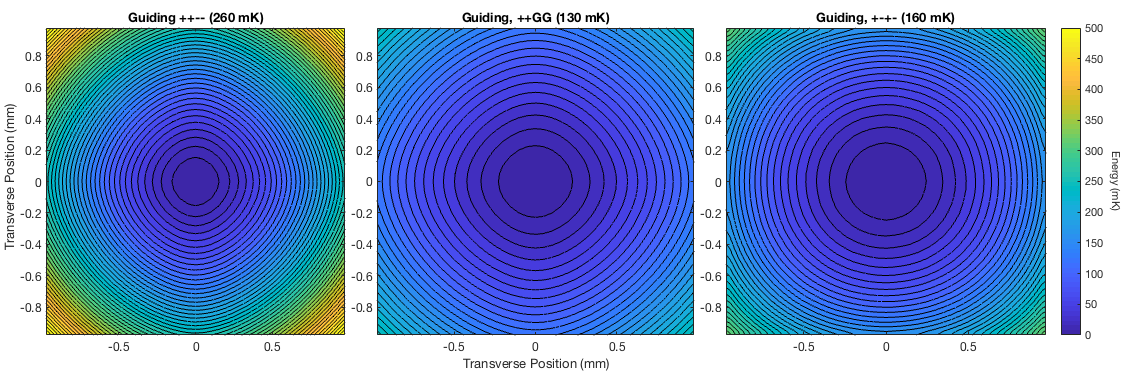
\includegraphics[width=\linewidth]{Slowing/guiding_compilation.png}
\caption[Transverse Guiding Potentials]{\label{fig:guiding_compilation}
Transverse Traps formed by Different Field Distributions. Field distributions are generated in COMSOL, converted to internal potential energy, and then averaged longitudinally.}
\end{figure}


Breathing modes were detected as expected, and an effort was undertaken to infer the initial population generated by the valve from the observed oscillations.
This turned out to serve as a probe of skimmer interference, since it was found that a distant source of the expected temperature could not reproduce the shallowness of the oscillation amplitude observed, although there are of course other deviations between model and experiment which could lead to a reduction in fringe contrast.
It was also found that by intentionally turning the trap off at the right moment could serve as a manipulation of the transverse phase space distribution for the sake of reduced transverse temperature.

It would be ideal to use this technique also as a means of studying the transverse or longitudinal frequencies in the traveling potential well in deceleration mode, but this has not yet been undertaken. 
Greater signal to noise would be desirable, at the time of this writing unavailable due to intentional space added between the source and the decelerator for studying collisions between parallel plates.

\section{Non-adiabatic Transitions}\label{sec:spinflipdecel}

The Landau-Zener formula may be used to approximate the relevance of non-adiabatic transitions in a given situation:
\begin{equation}
P=e^{-\pi\Delta^2/\hbar\frac{\partial E}{\partial t}}.
\end{equation}
Working in frequency units, we can simplify this to say that non-adiabatic transitions are negligible provided that:
\begin{equation}
g >> \sqrt{e\cdot f},
\end{equation}
where $g$ is the closest approach of the states, $e$ is the average energy difference between the relevant states during the process of interest, and $f$ is the frequency characterizing the variation of the system over time.
This is a convenient rule of thumb- just compare the minimum gap to the geometric mean of the typical energy scale and the inverse timescale.

For example, in the absence of any magnetic field, parity flips from $|f\rangle$ to $|e\rangle$ are highly unlikely thanks to the lambda doublet spacing of $1.7$~GHz.
Compare this with the geometric mean of $100$~GHz and $1$~MHz where the latter is appropriate for the microsecond turn-off of the fields during switching events and the former is the energy scale set by the magnitude of electric fields in the decelerator.
We find $300$~MHz or so, getting close to $1.7$~GHz but still below.

On the other hand, transitions between \f3 and \f1 are a much greater concern, and have been observed during propagation of molecules in decelerators~\cite{Meek2011}, and also during switching events of decelerators~\cite{Wall2010}.
The Stark effect treats \fpm3 the same, and also \fpm1, but the latter have one third the response of the former, so transitions between them are essentially loss.
Moreover, these states are degenerate at zero field and don't have any fixed barrier as do the states of different parity.
Of course, states being degenerate does not necessarily lead to loss if the Hamiltonian driving their evolution does not have any amplitude connecting the states in question.
For states of differing $m$ quantum number, the Hamiltonian will only couple them when molecules are experiencing a rotation of the electric field vector.
In S\,=\,1 operation, suitably fast rotations, together with very small values of the electric field, cannot occur on-axis, but may occur for off-axis molecules that experience weaker fields close to the grounded decelerator pins.
I investigated the loss probability for off-axis molecules, for the first time as far as I can tell, and the results I obtained are shown in Fig.~\ref{non-adiabatic1}.
Only a small fraction of molecules are lost, perhaps something like $0.1\%$ over the length of the decelerator.
Being more quantitative would require simulating a denser grid of trajectories close to the pins.

\begin{figure}[t!]
\centering
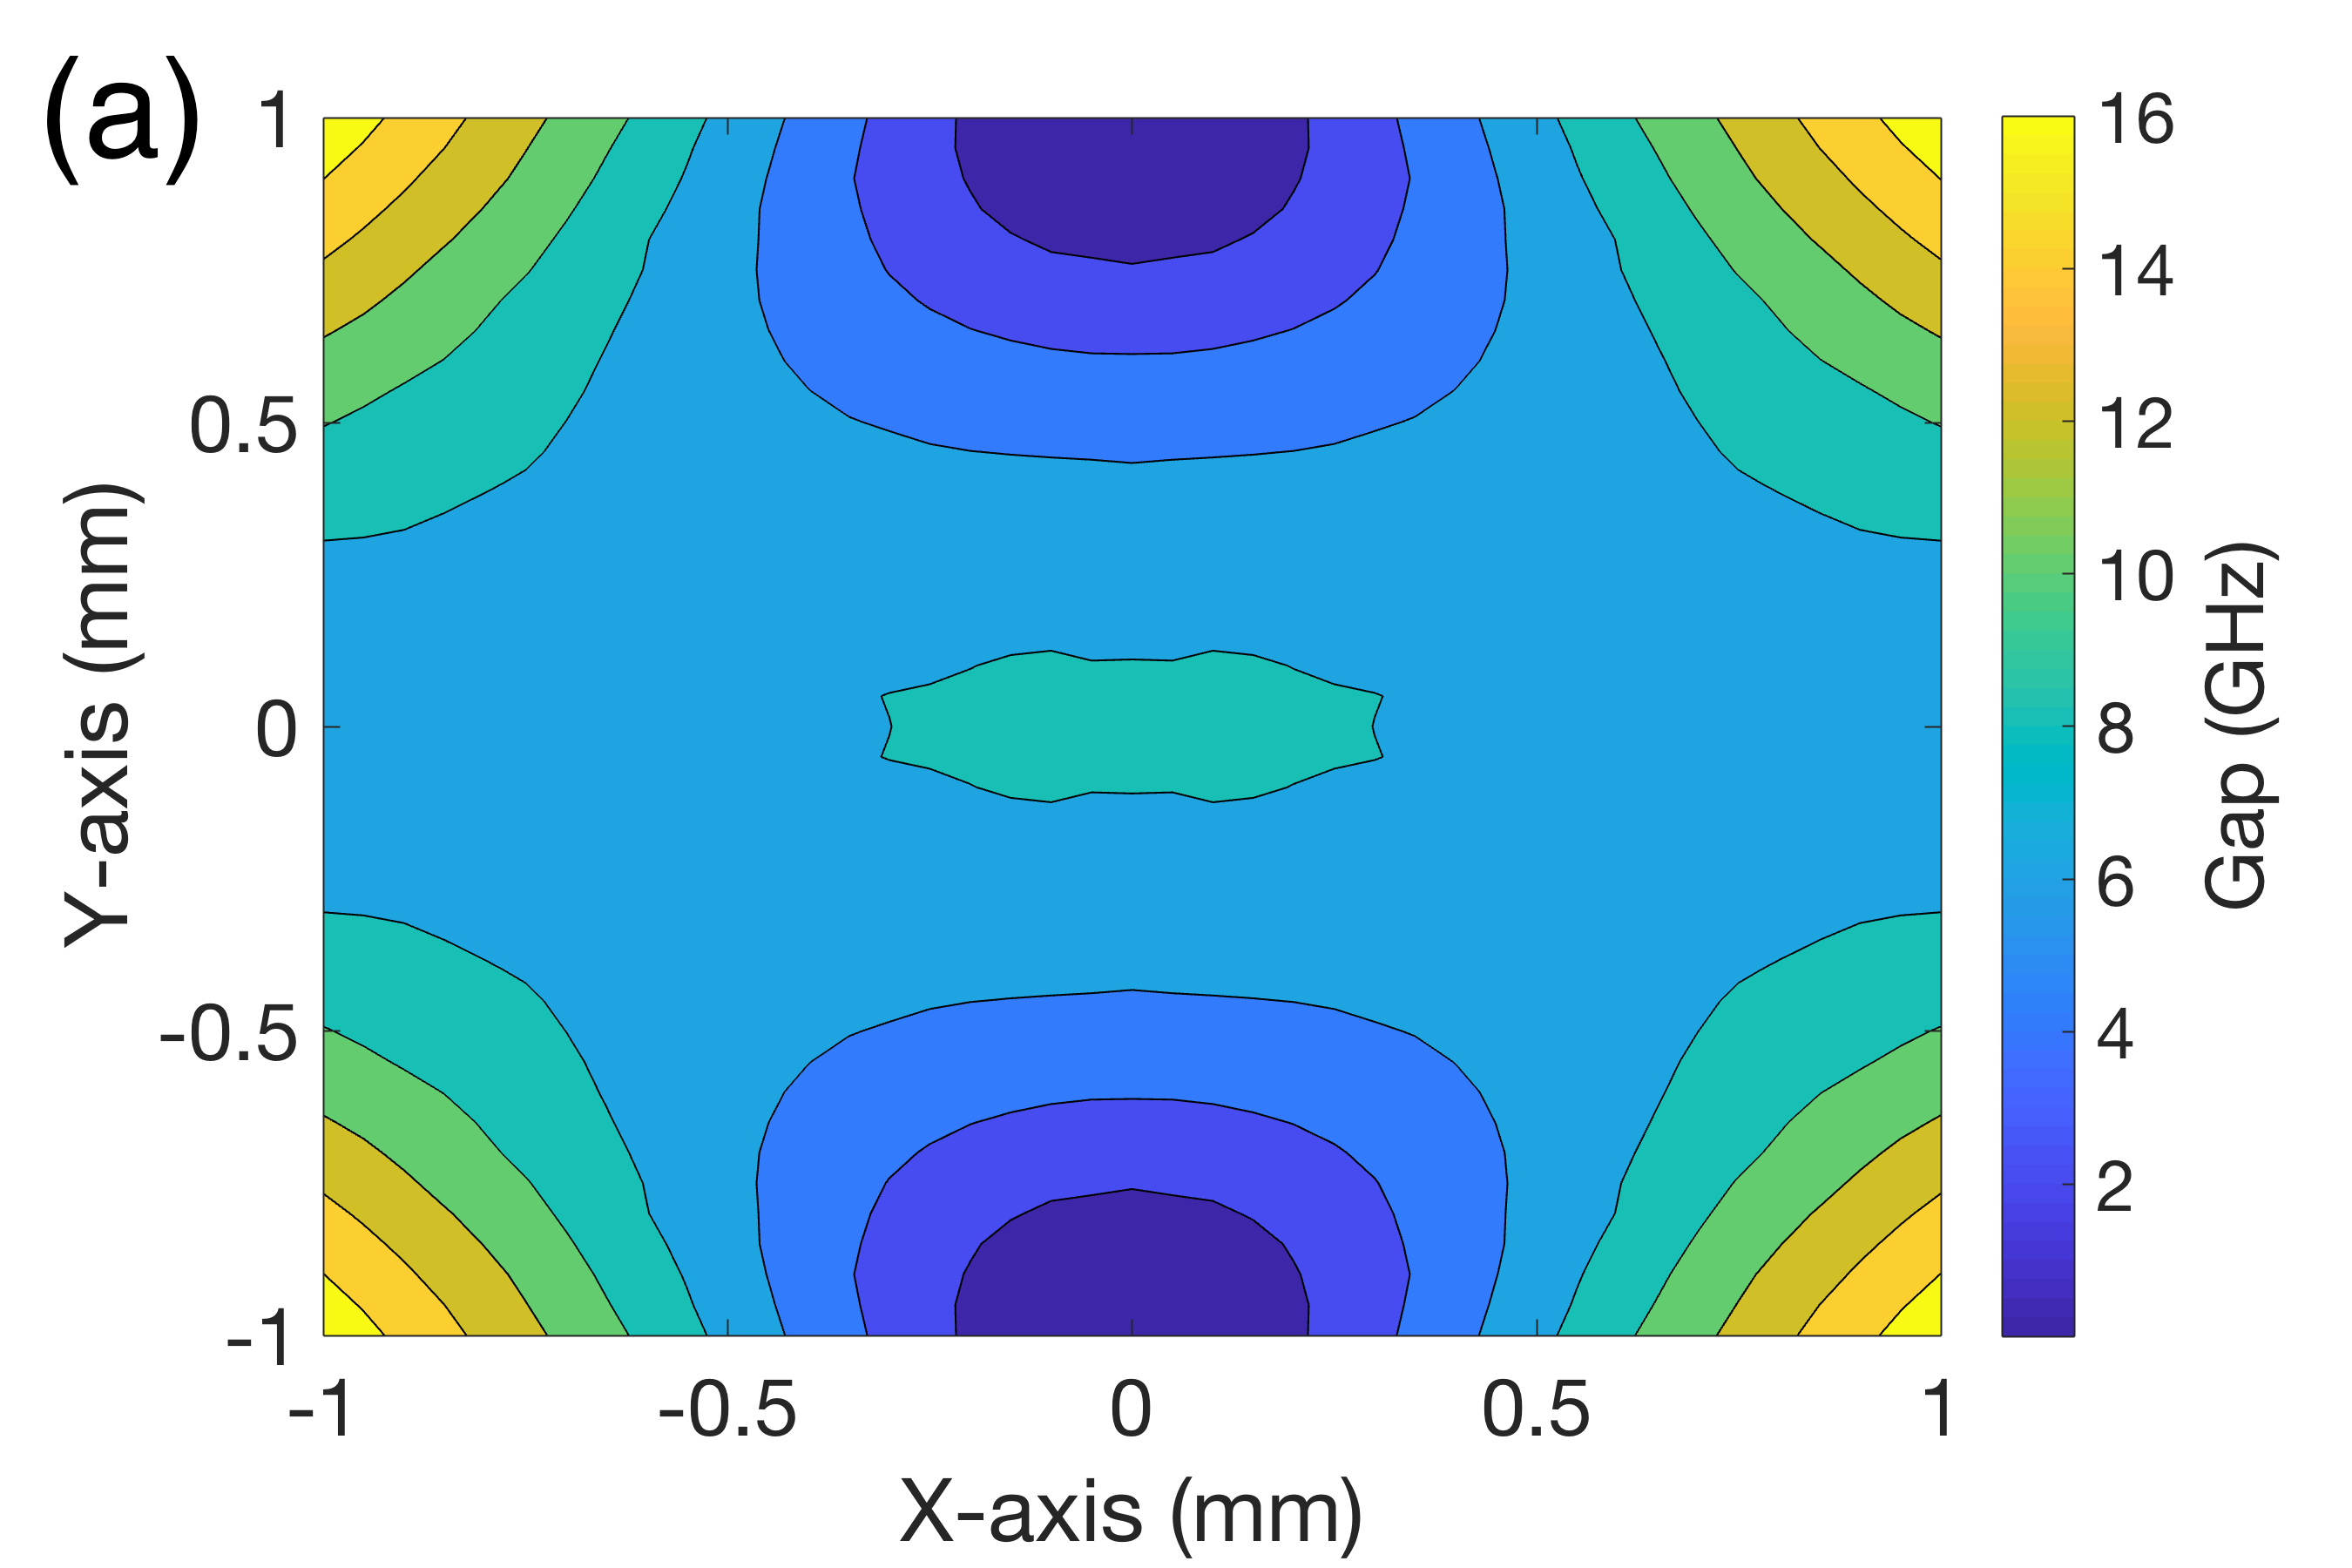
\includegraphics[width=8cm]{StarkGap.png}
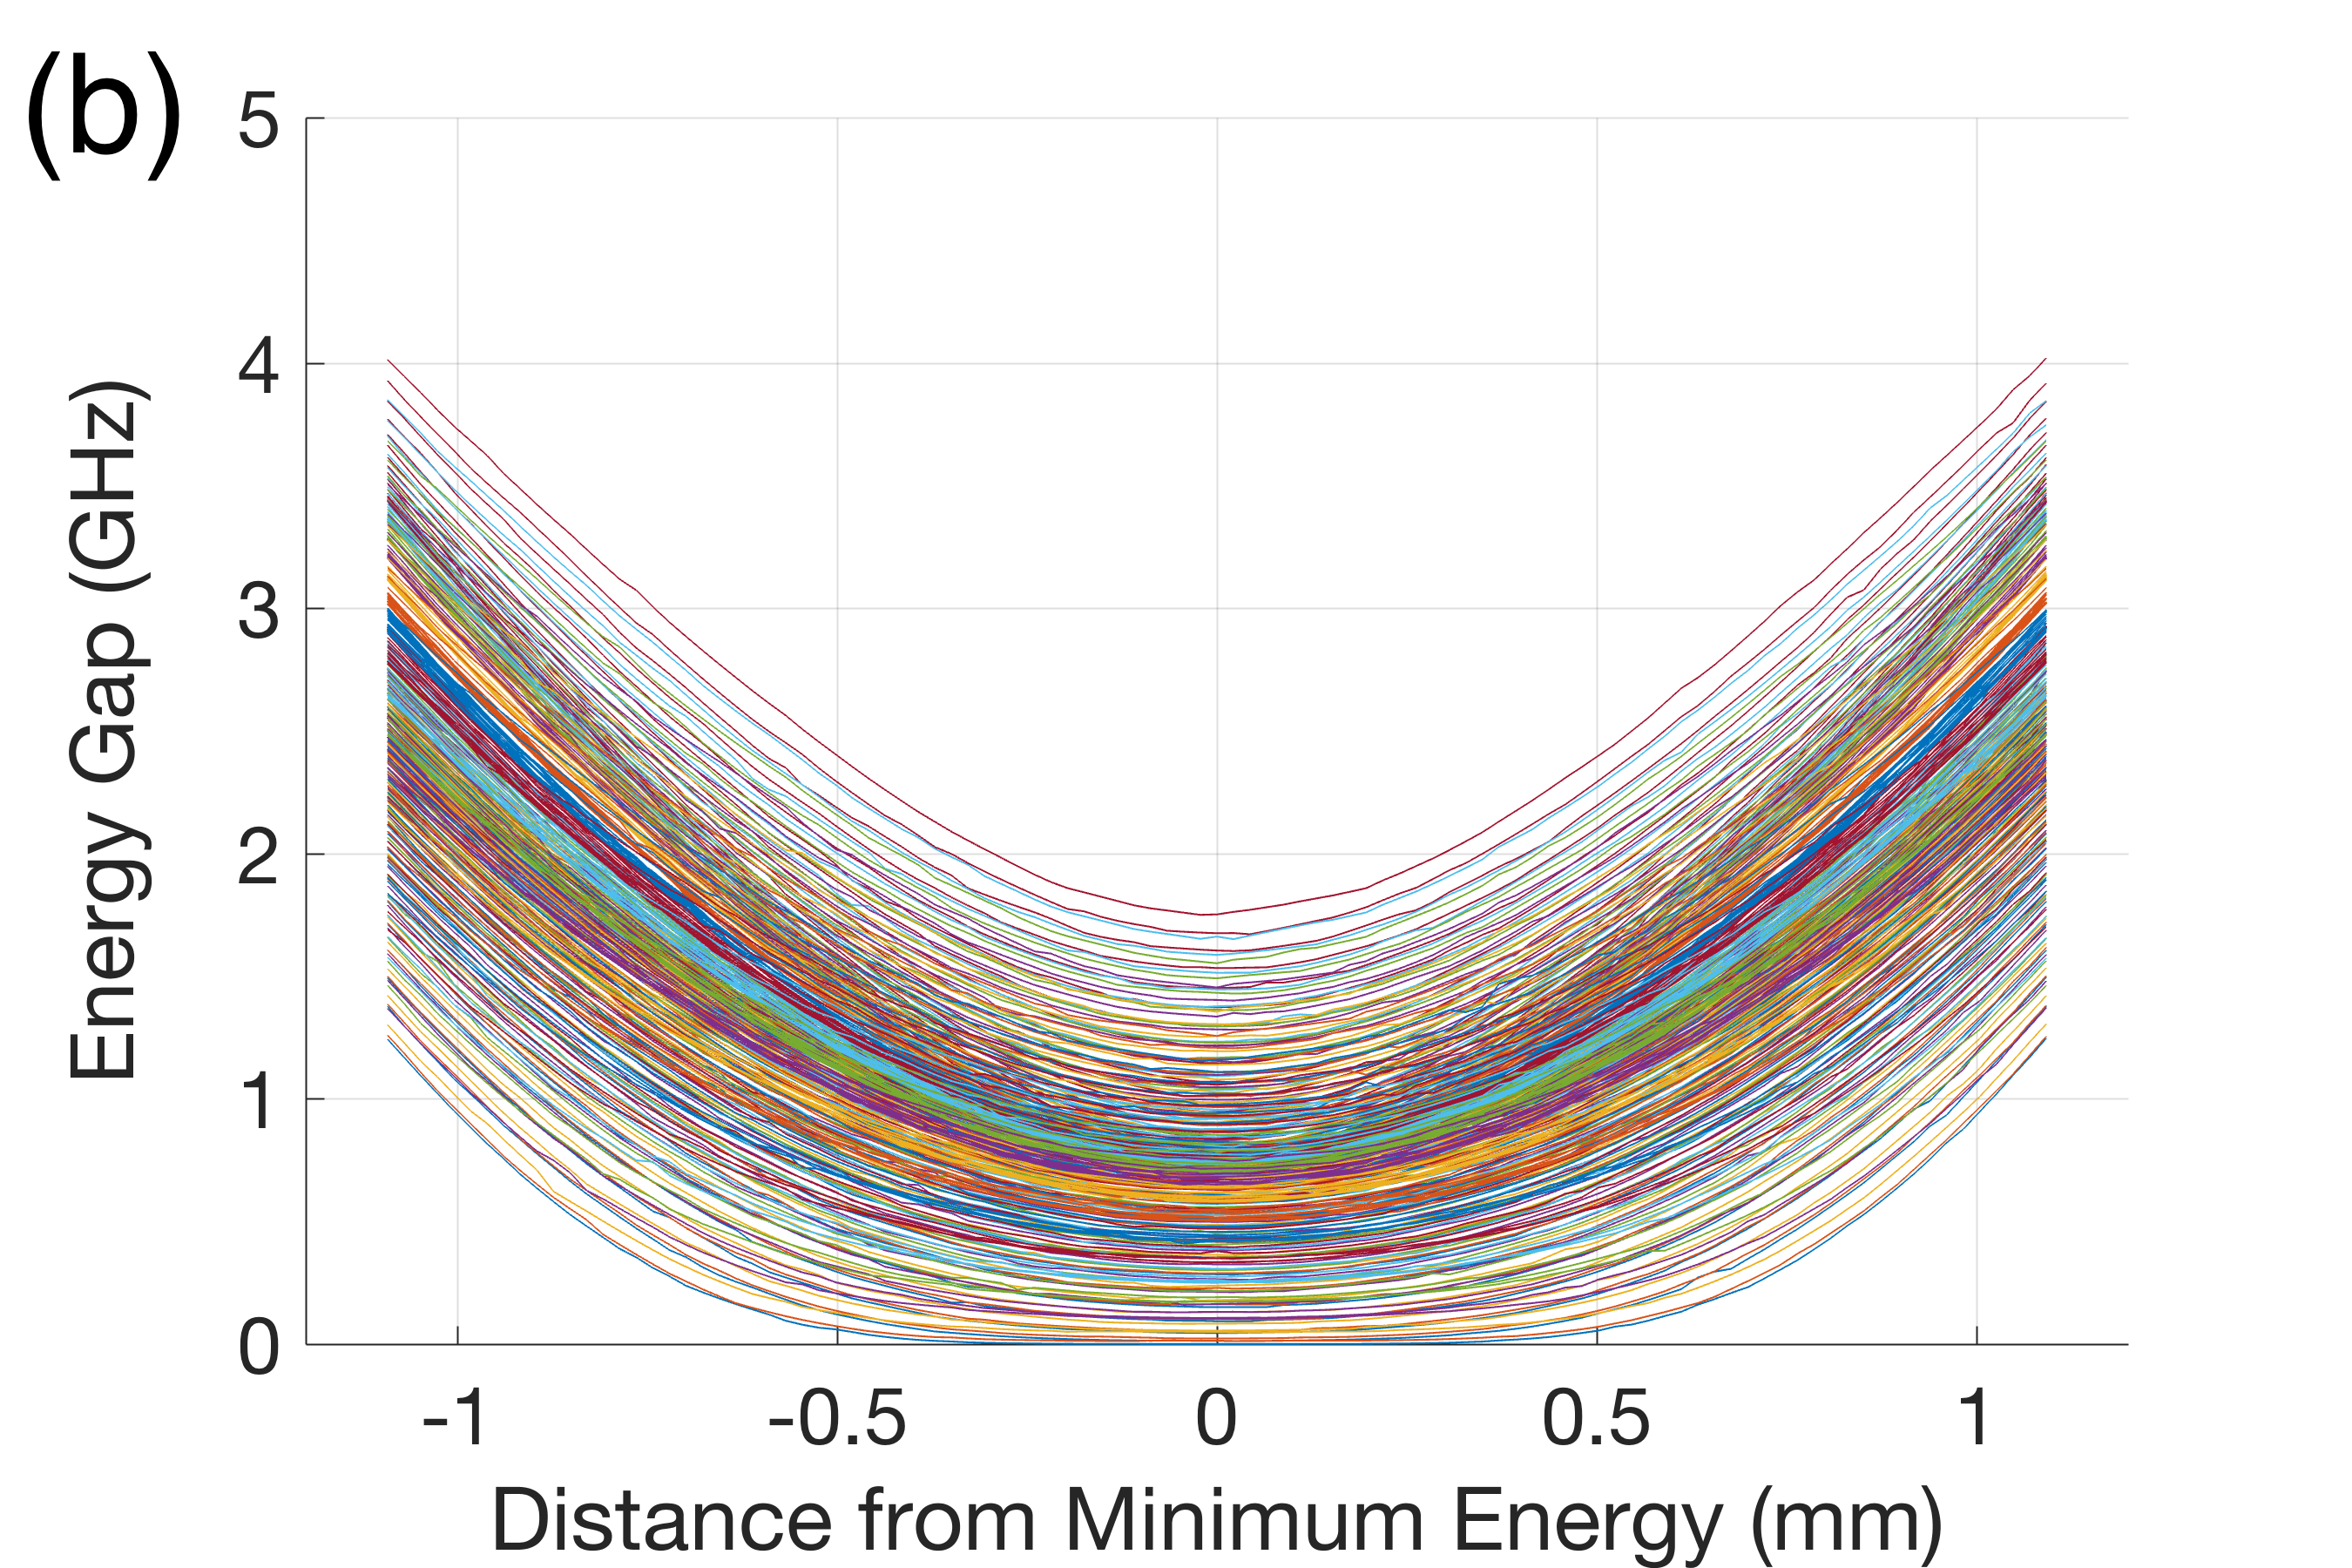
\includegraphics[width=8cm]{NonadTraj.png}\\
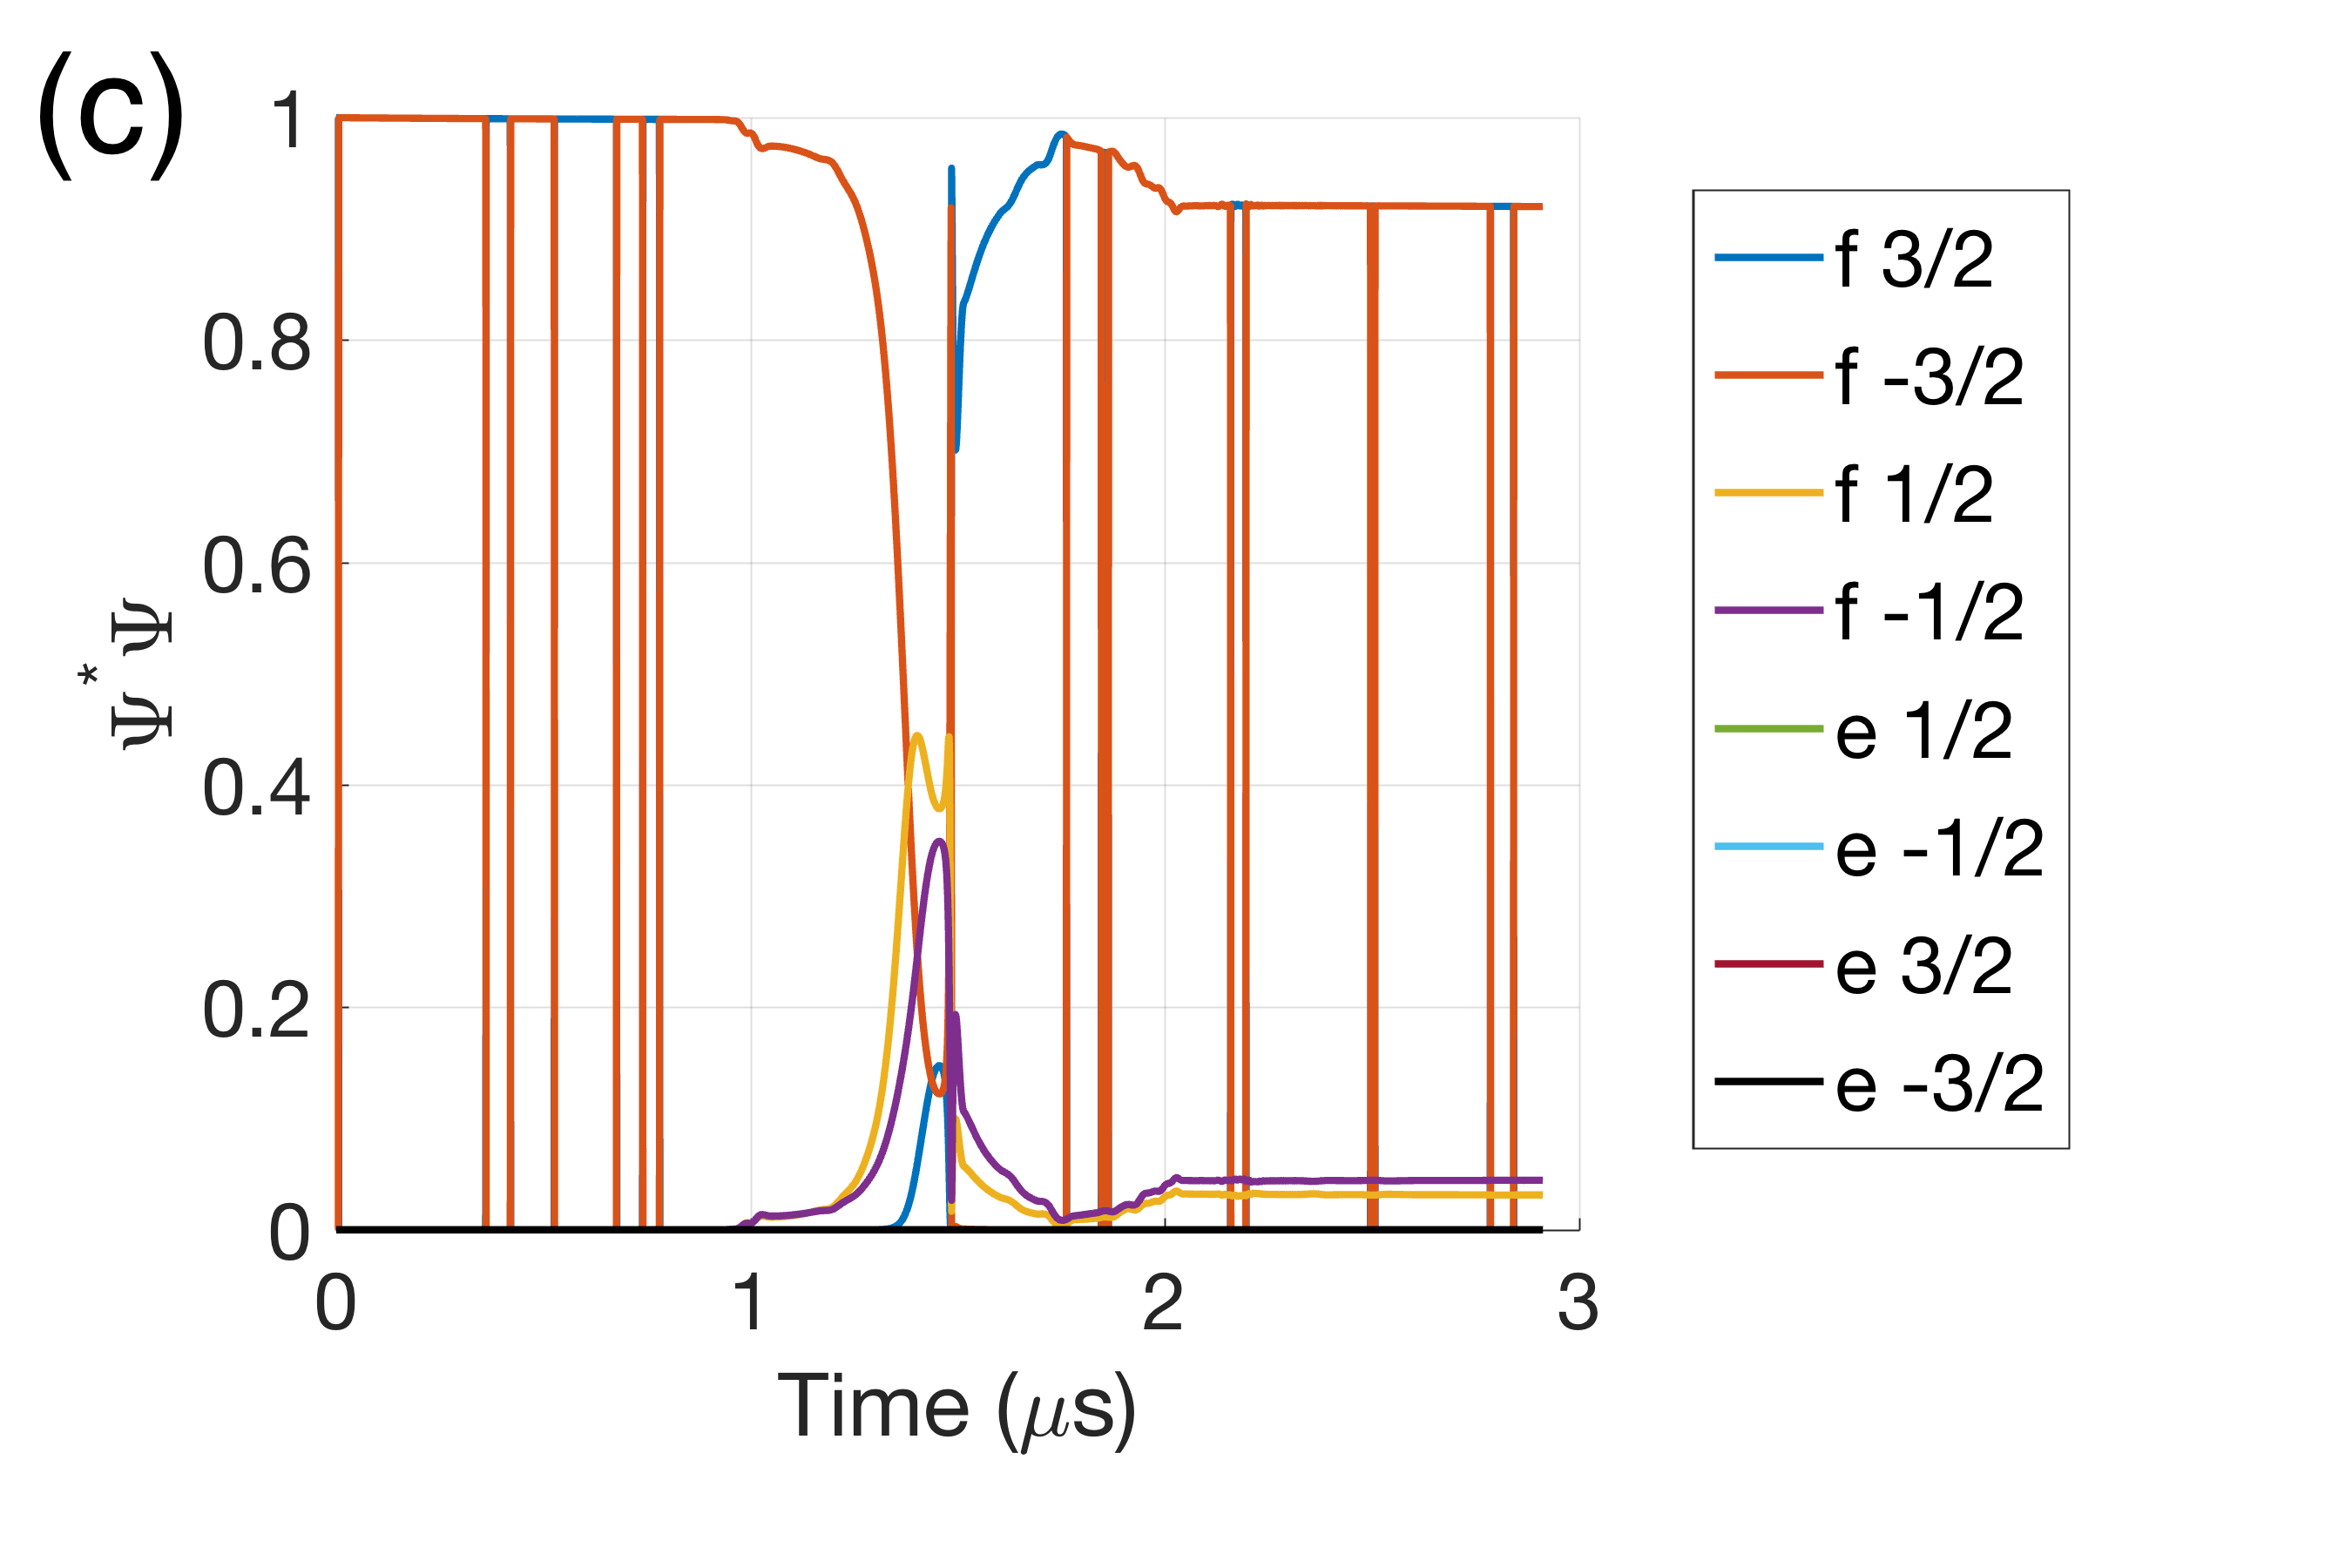
\includegraphics[width=8cm]{SampleTISE.png}
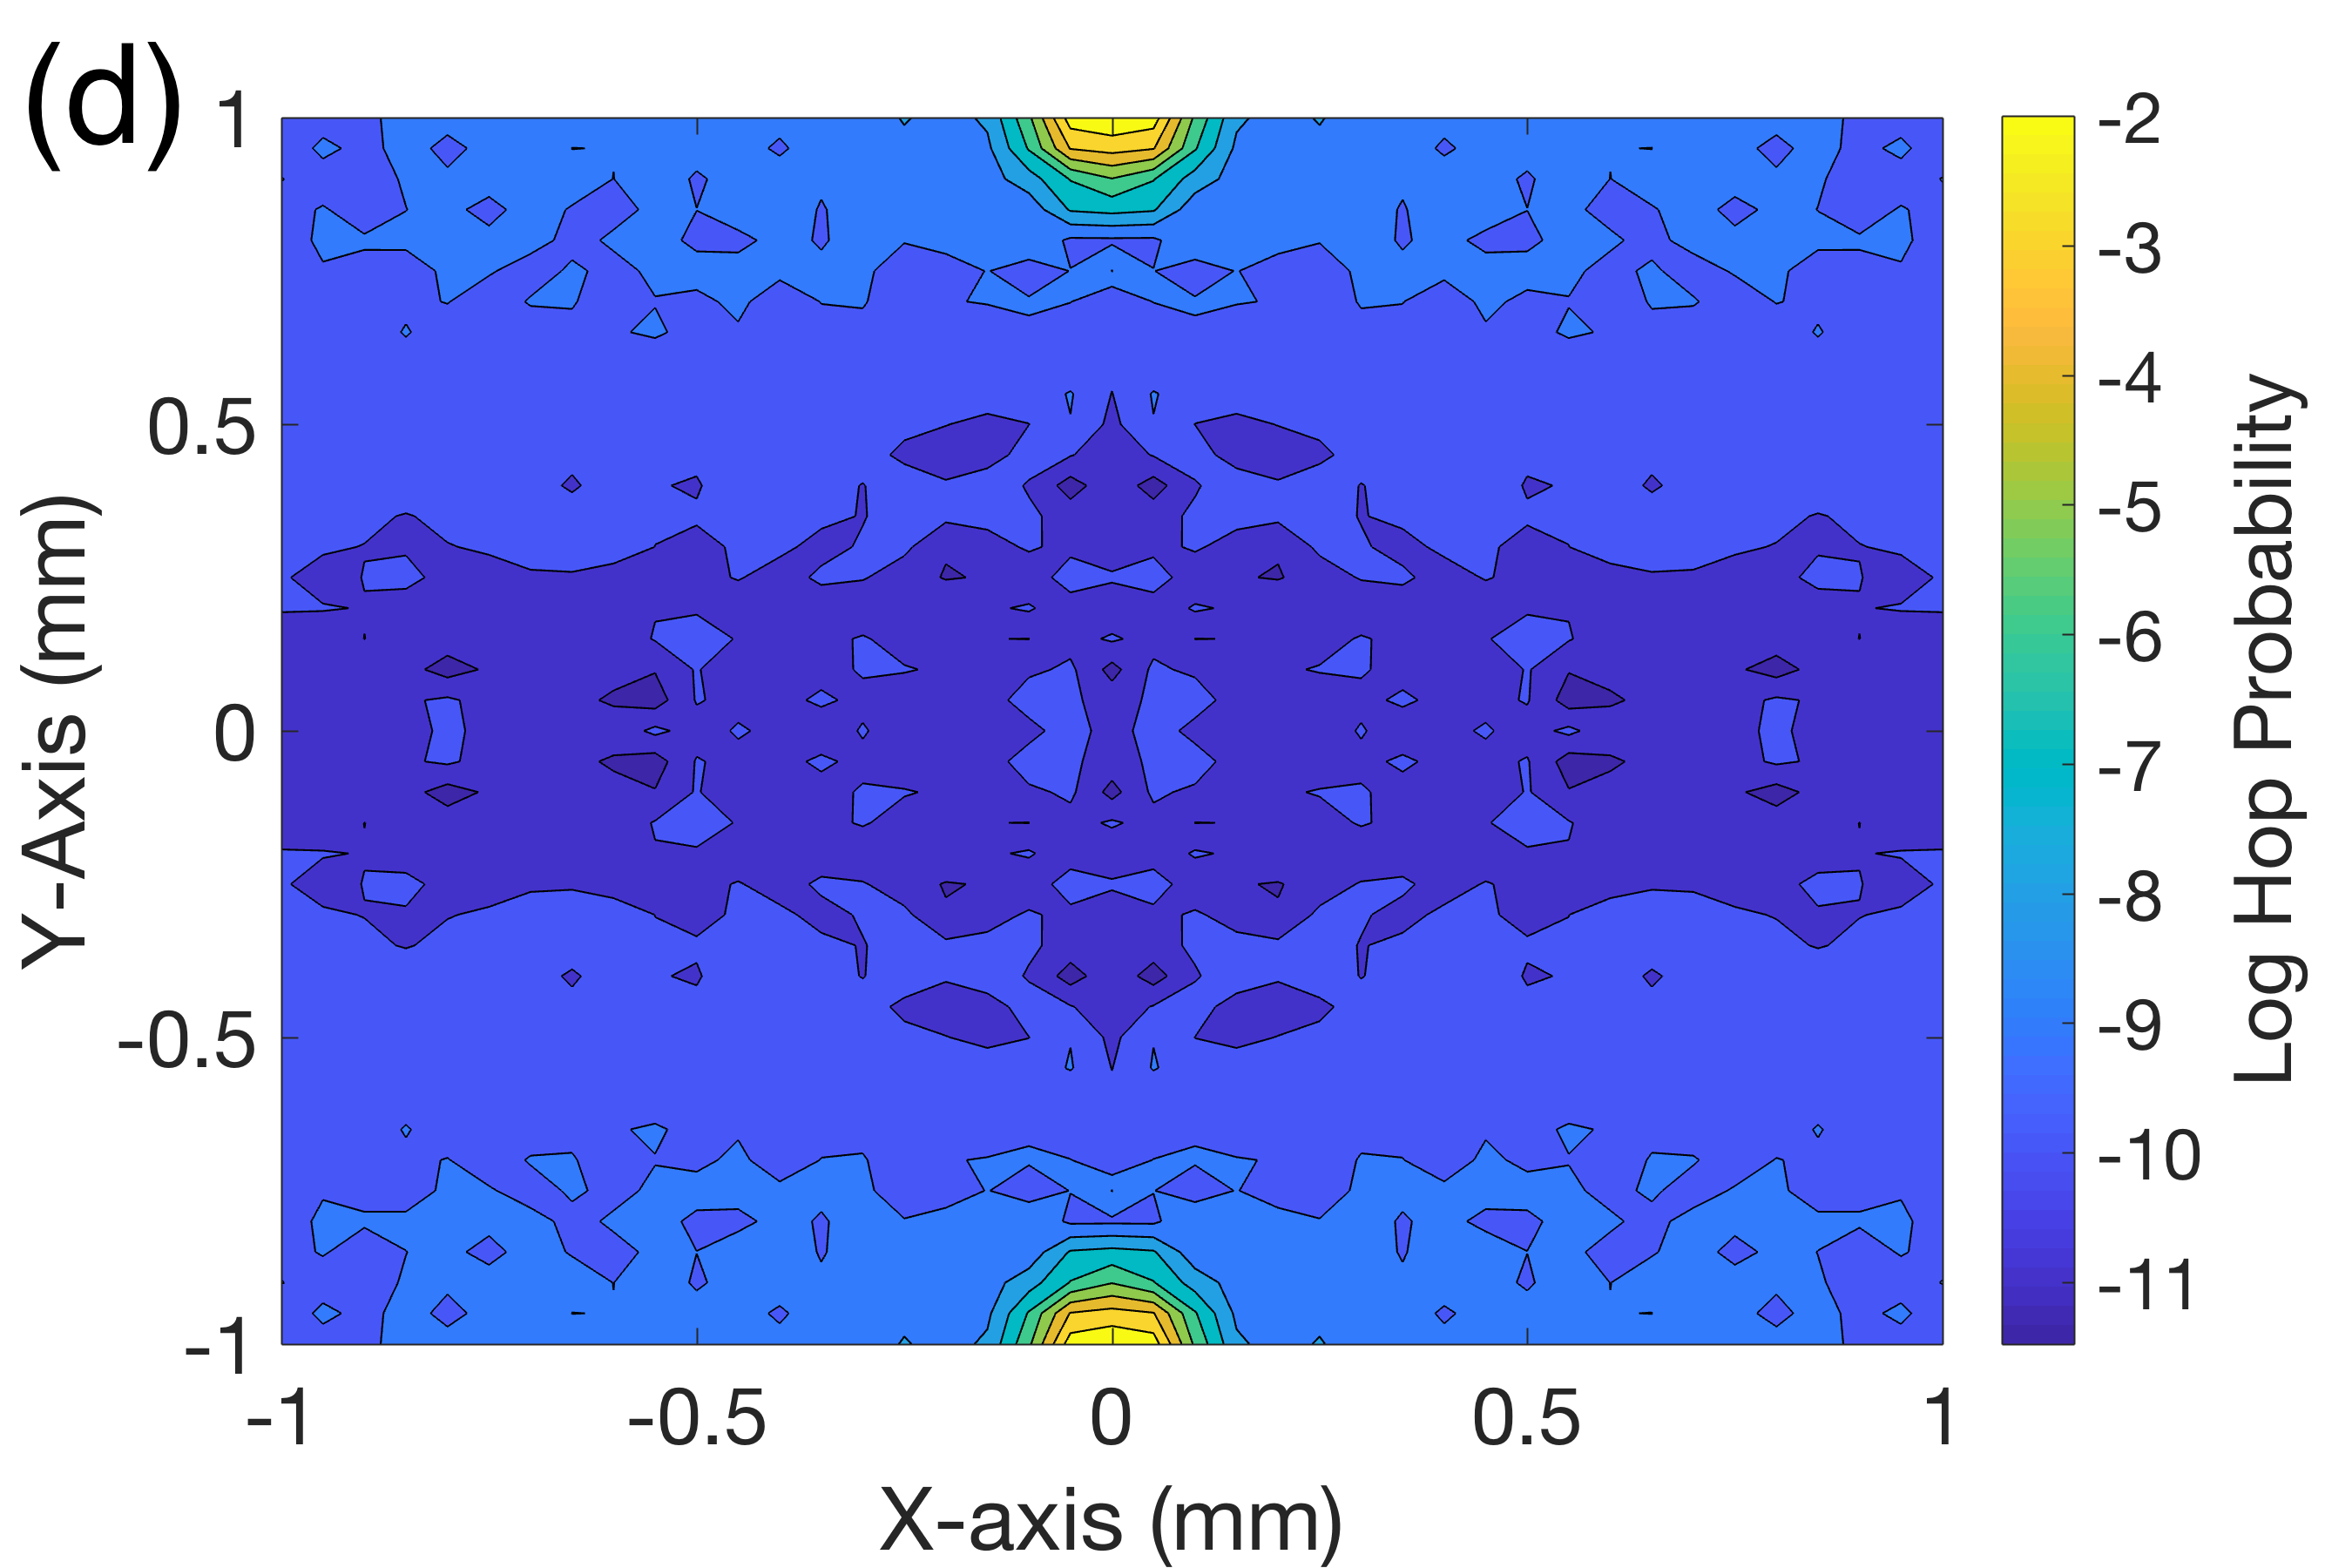
\includegraphics[width=8cm]{AllProb.png}
\caption[Non-adiabatic Transitions Off-Axis]{\label{non-adiabatic1}
(a) Minimum energy gap along straight line trajectories parallel to decelerator axis and intersecting the transverse plane as shown. (b) Resulting energy gap as a function of propagation distance for a grid of trajectories. (c) Sample solution of the time-independent Schr\"{o}dinger equation for a trajectory that shows a $10\%$ chance of hopping to the \f1 state. Many sharp jumps are seen between \fpm3, these are irrelevant and an artifact of an unphysically small bias magnetic field. (d) Inferred hopping probability as a function of position in the transverse plane.
}
\end{figure}

Even if free propagation doesn't lead to non-adiabatic transitions even off axis, there is still the question of non-adiabatic transitions during the switching of the electric fields.
I also checked this, for the first time as best I can tell, for a 3D grid of possible positions relative to the synchronous molecule, see Fig.~\ref{nonadiabatic2}.
I find that non-adiabatic transitions are possible only if the molecule is significantly behind the synchronous molecule, shielded by the grounded pins just prior to their being rapidly switched on.
These positions are not longitudinally phase stable anyway, unless the decelerator is being operated in an acceleration mode, in which case some locations off axis do seem to feature a significant chance of non-adiabatic transitions.
\begin{figure}[t!]
\centering
\vspace{0.5mm}
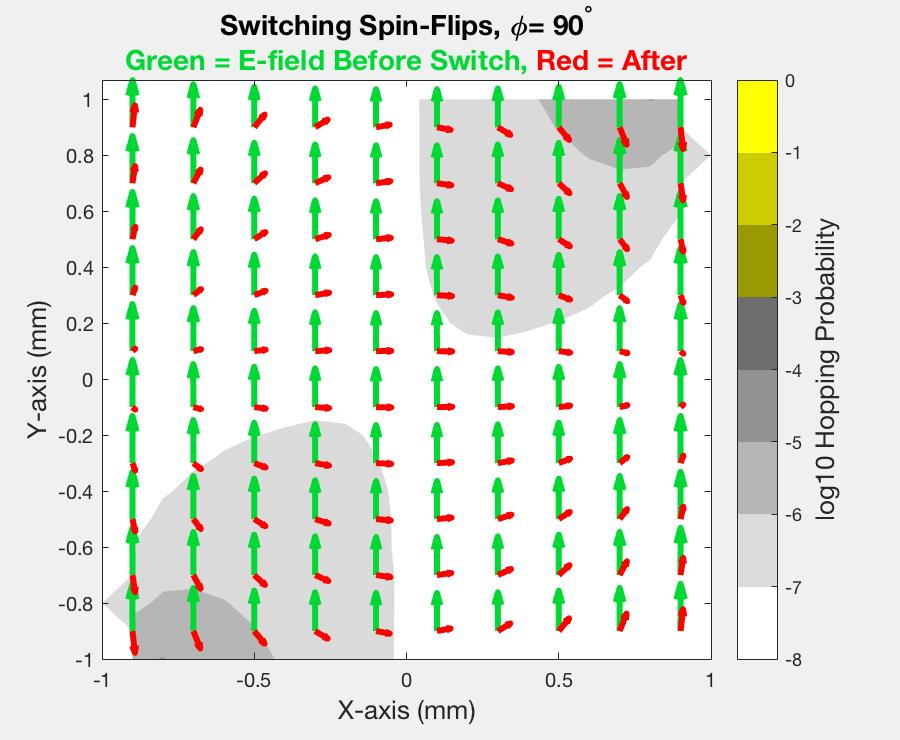
\includegraphics[width=7.5cm]{switchloss1.png}
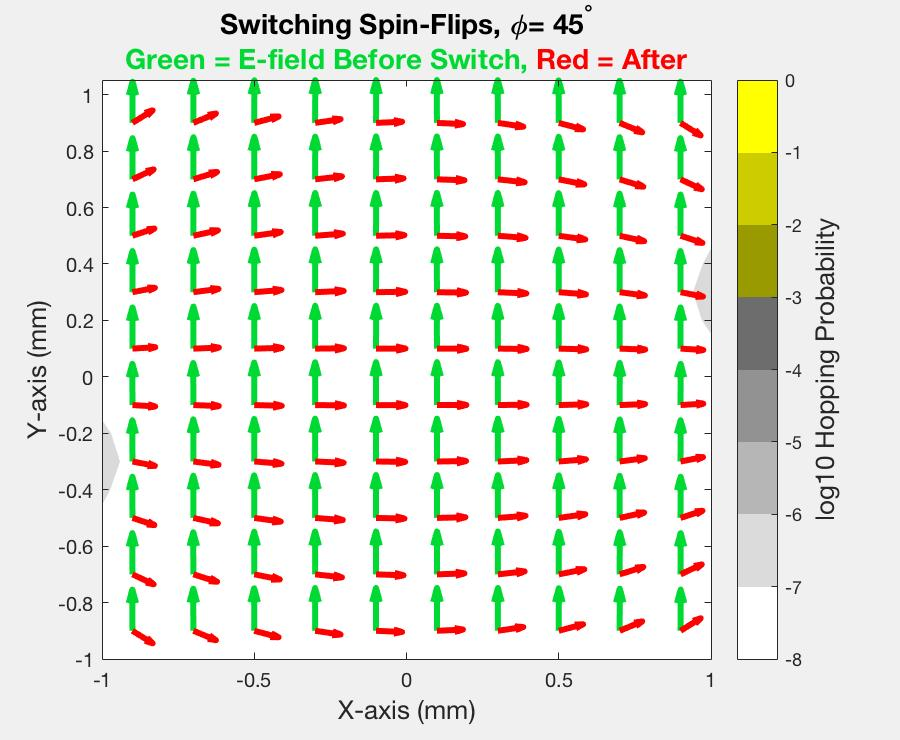
\includegraphics[width=7.5cm]{switchloss2.png}\\
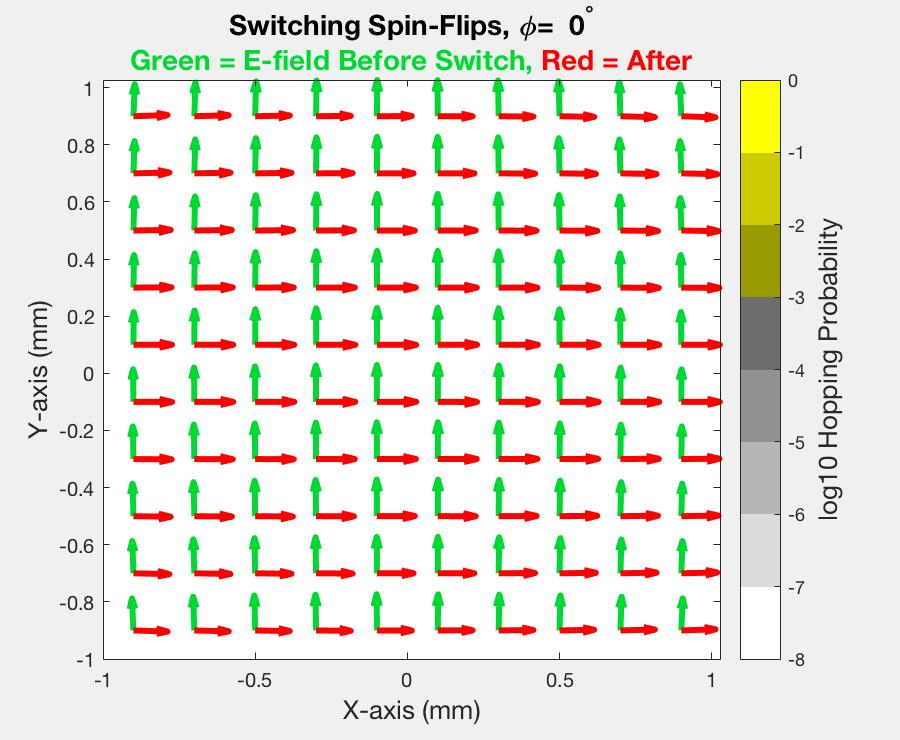
\includegraphics[width=7.5cm]{switchloss3.png}
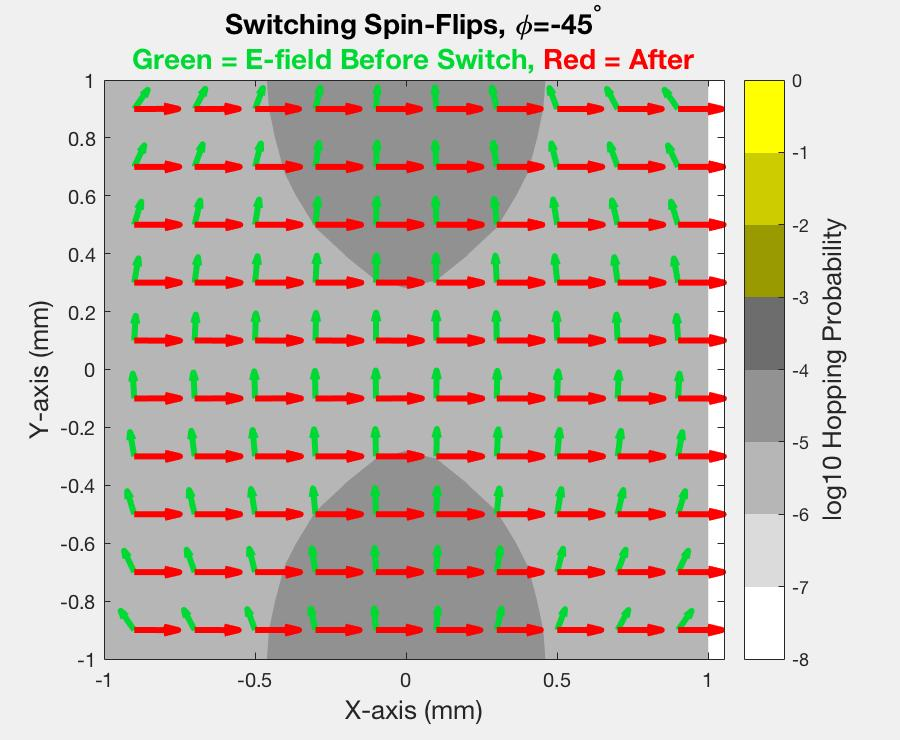
\includegraphics[width=7.5cm]{switchloss4.png}\\
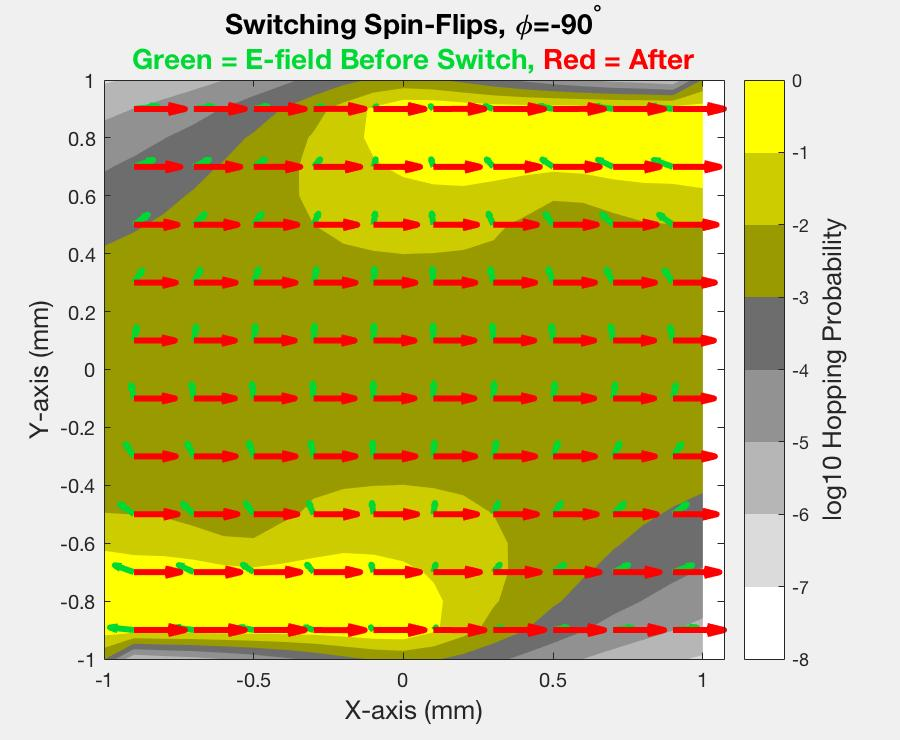
\includegraphics[width=7.5cm]{switchloss5.png}
\caption[Non-adiabatic Losses during Switching]{\label{nonadiabatic2}
Loss per switching event in several $x-y$ planes of different $z$ coordinate parametrized by phase angle $\phi=90^\circ$, $45^\circ$, $0^\circ$, $-45^\circ$, and $-90^\circ$, from left to right and top to bottom.
Significant loss only in the $-90^\circ$ plane, where phase stable molecules do not reside anyway.}
\end{figure}
The real thing to do would be to repeat this study with alternate field distributions in mind.
These would be likely to feature a significantly enhanced chance of free propagation transitions close to the electric quadrupole created by the alternate configurations between the grounded pin pair.
As far as the chance of switch-induced non-adiabatic transitions, those would seem to be reduced by the alternate field distributions, since in S\,=\,1 mode they were worst with the molecules beginning in a region of small field, and the alternate distributions generally add electric field in the regions where it was previously small or absent.
However significant the non-adiabatic transitions in the new operation modes, one way to address them is to intentionally vary the length of decelerator pins, so that one pin is longer than the other in a pair, see Fig.~\ref{offsetavoid}.
What this does is push the electric field zero off of the decelerator axis, creating some extra protective energy splitting even for molecules passing dangerously close to the field minimum.
At first pass, one might suspect that the field would be zero not at a point but along the line parallel to the grounded pin pair and in between the grounded pins.
This is approximately true as shown in Fig.~\ref{offsetavoid}a, but not perfectly so, as seen by examining the $\hat{y}$ component of the electric field as shown in Fig.~\ref{offsetavoid}b.
Thanks to the variation in length of our decelerator pins, an unintended side effect of tapered pin mounting as described in Sec.~\ref{sec:mechconsider}, our decelerator may benefit from reduced sensitivity to these spin-flip issues.

\begin{figure}[t!]
\centering
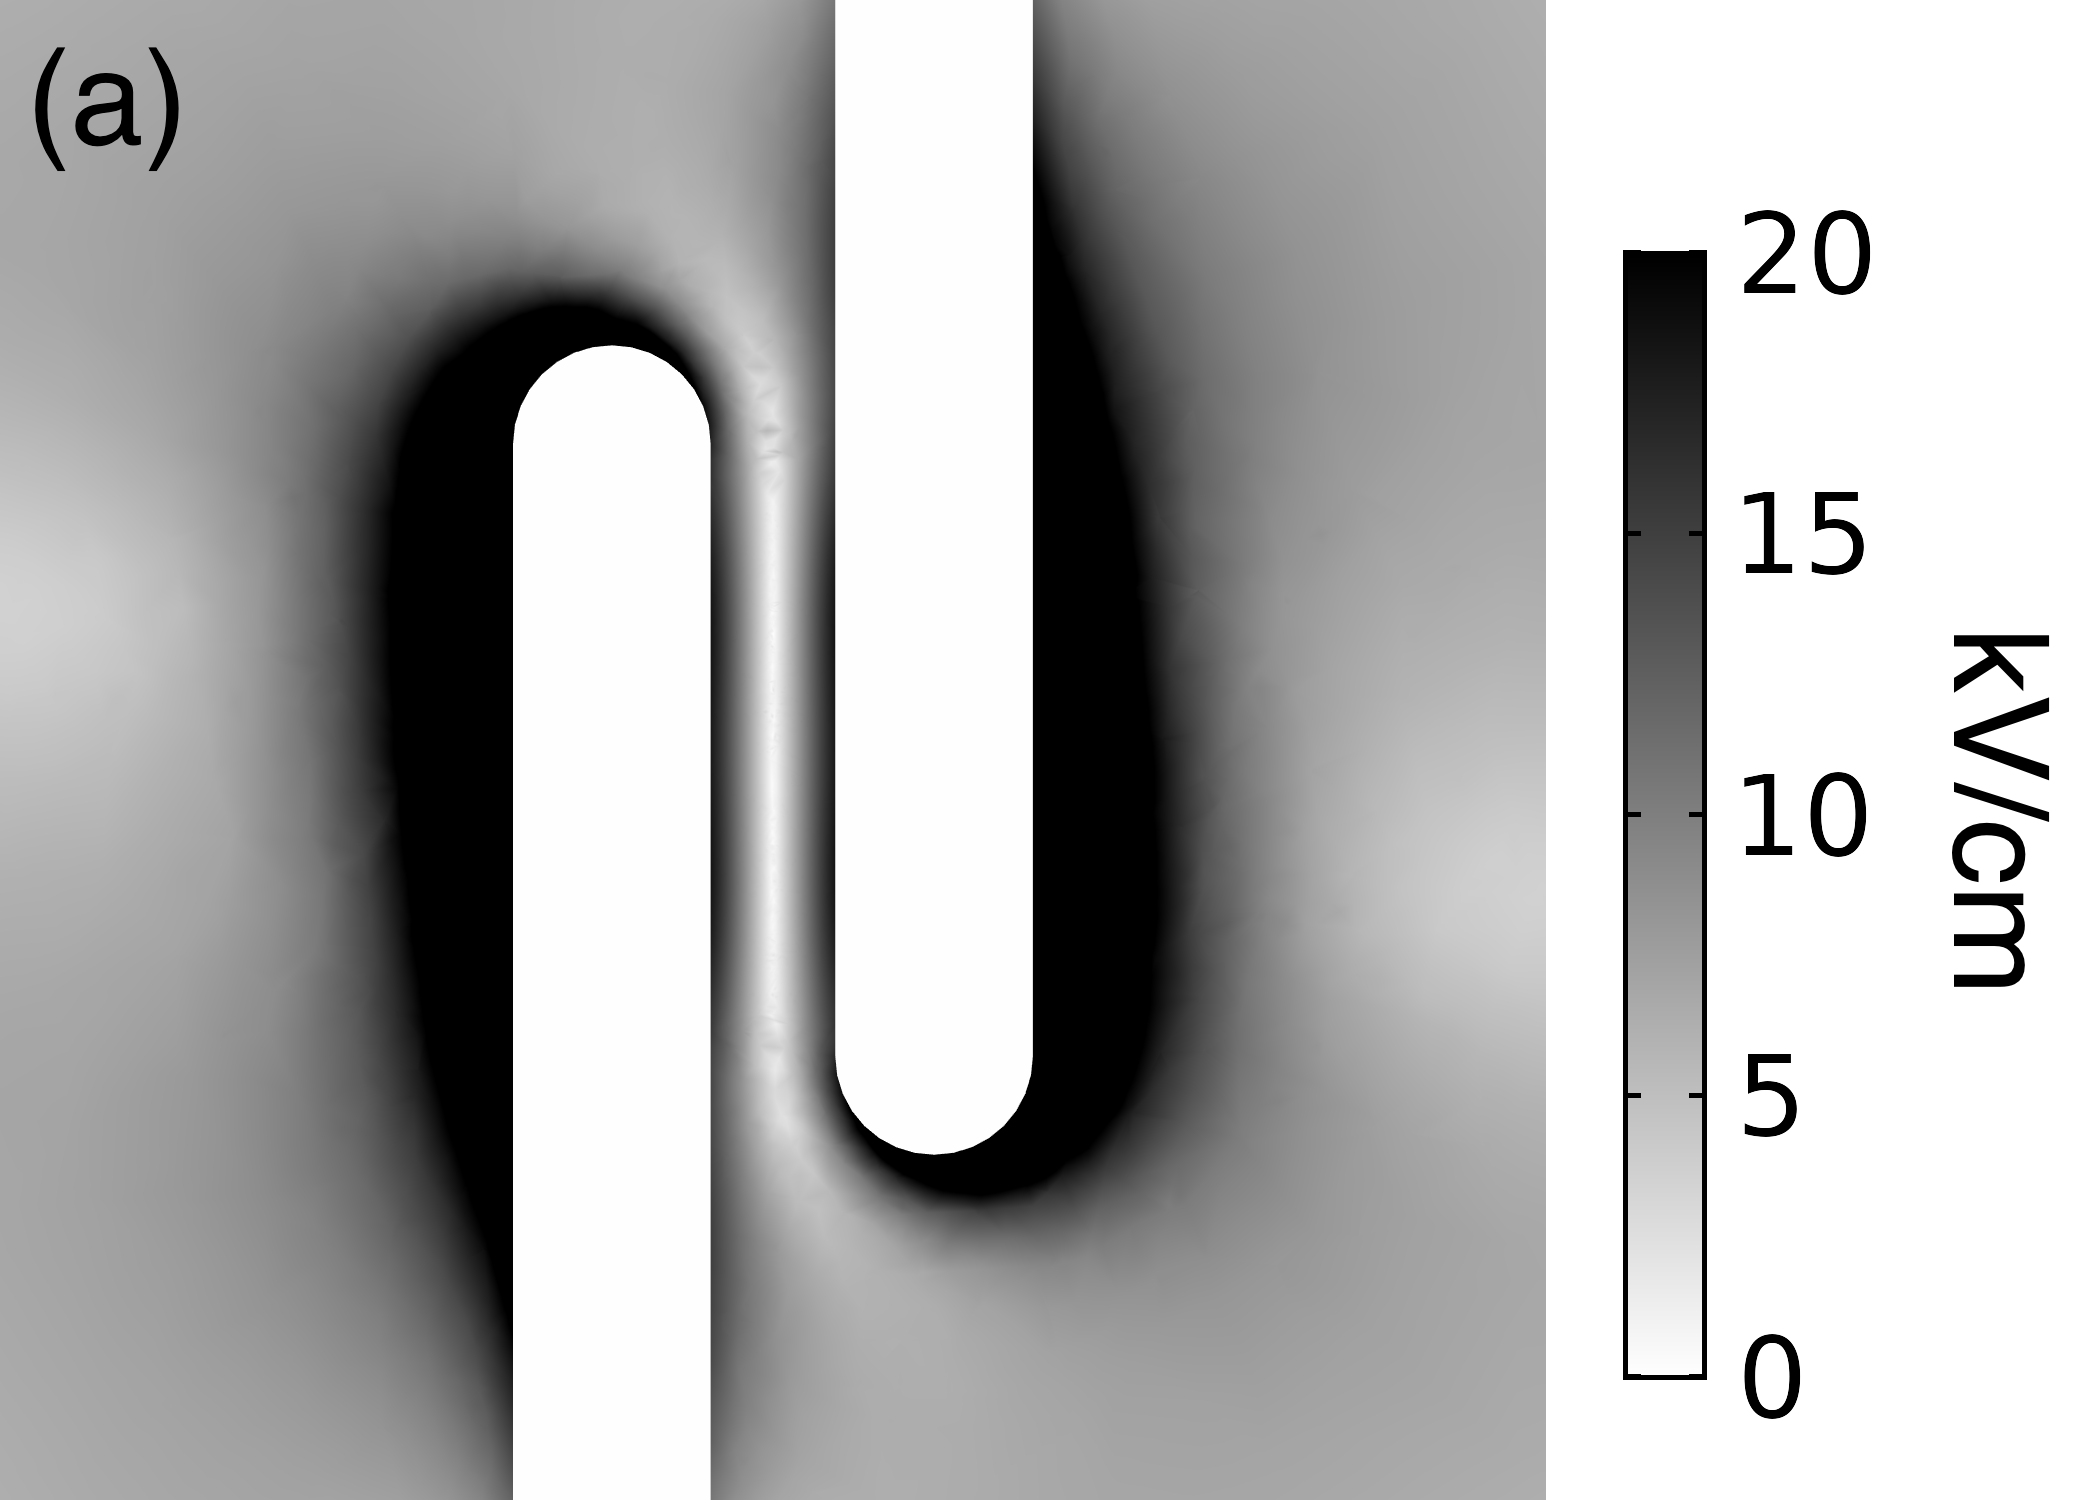
\includegraphics[width=8cm]{offset-avoid-loss.png}
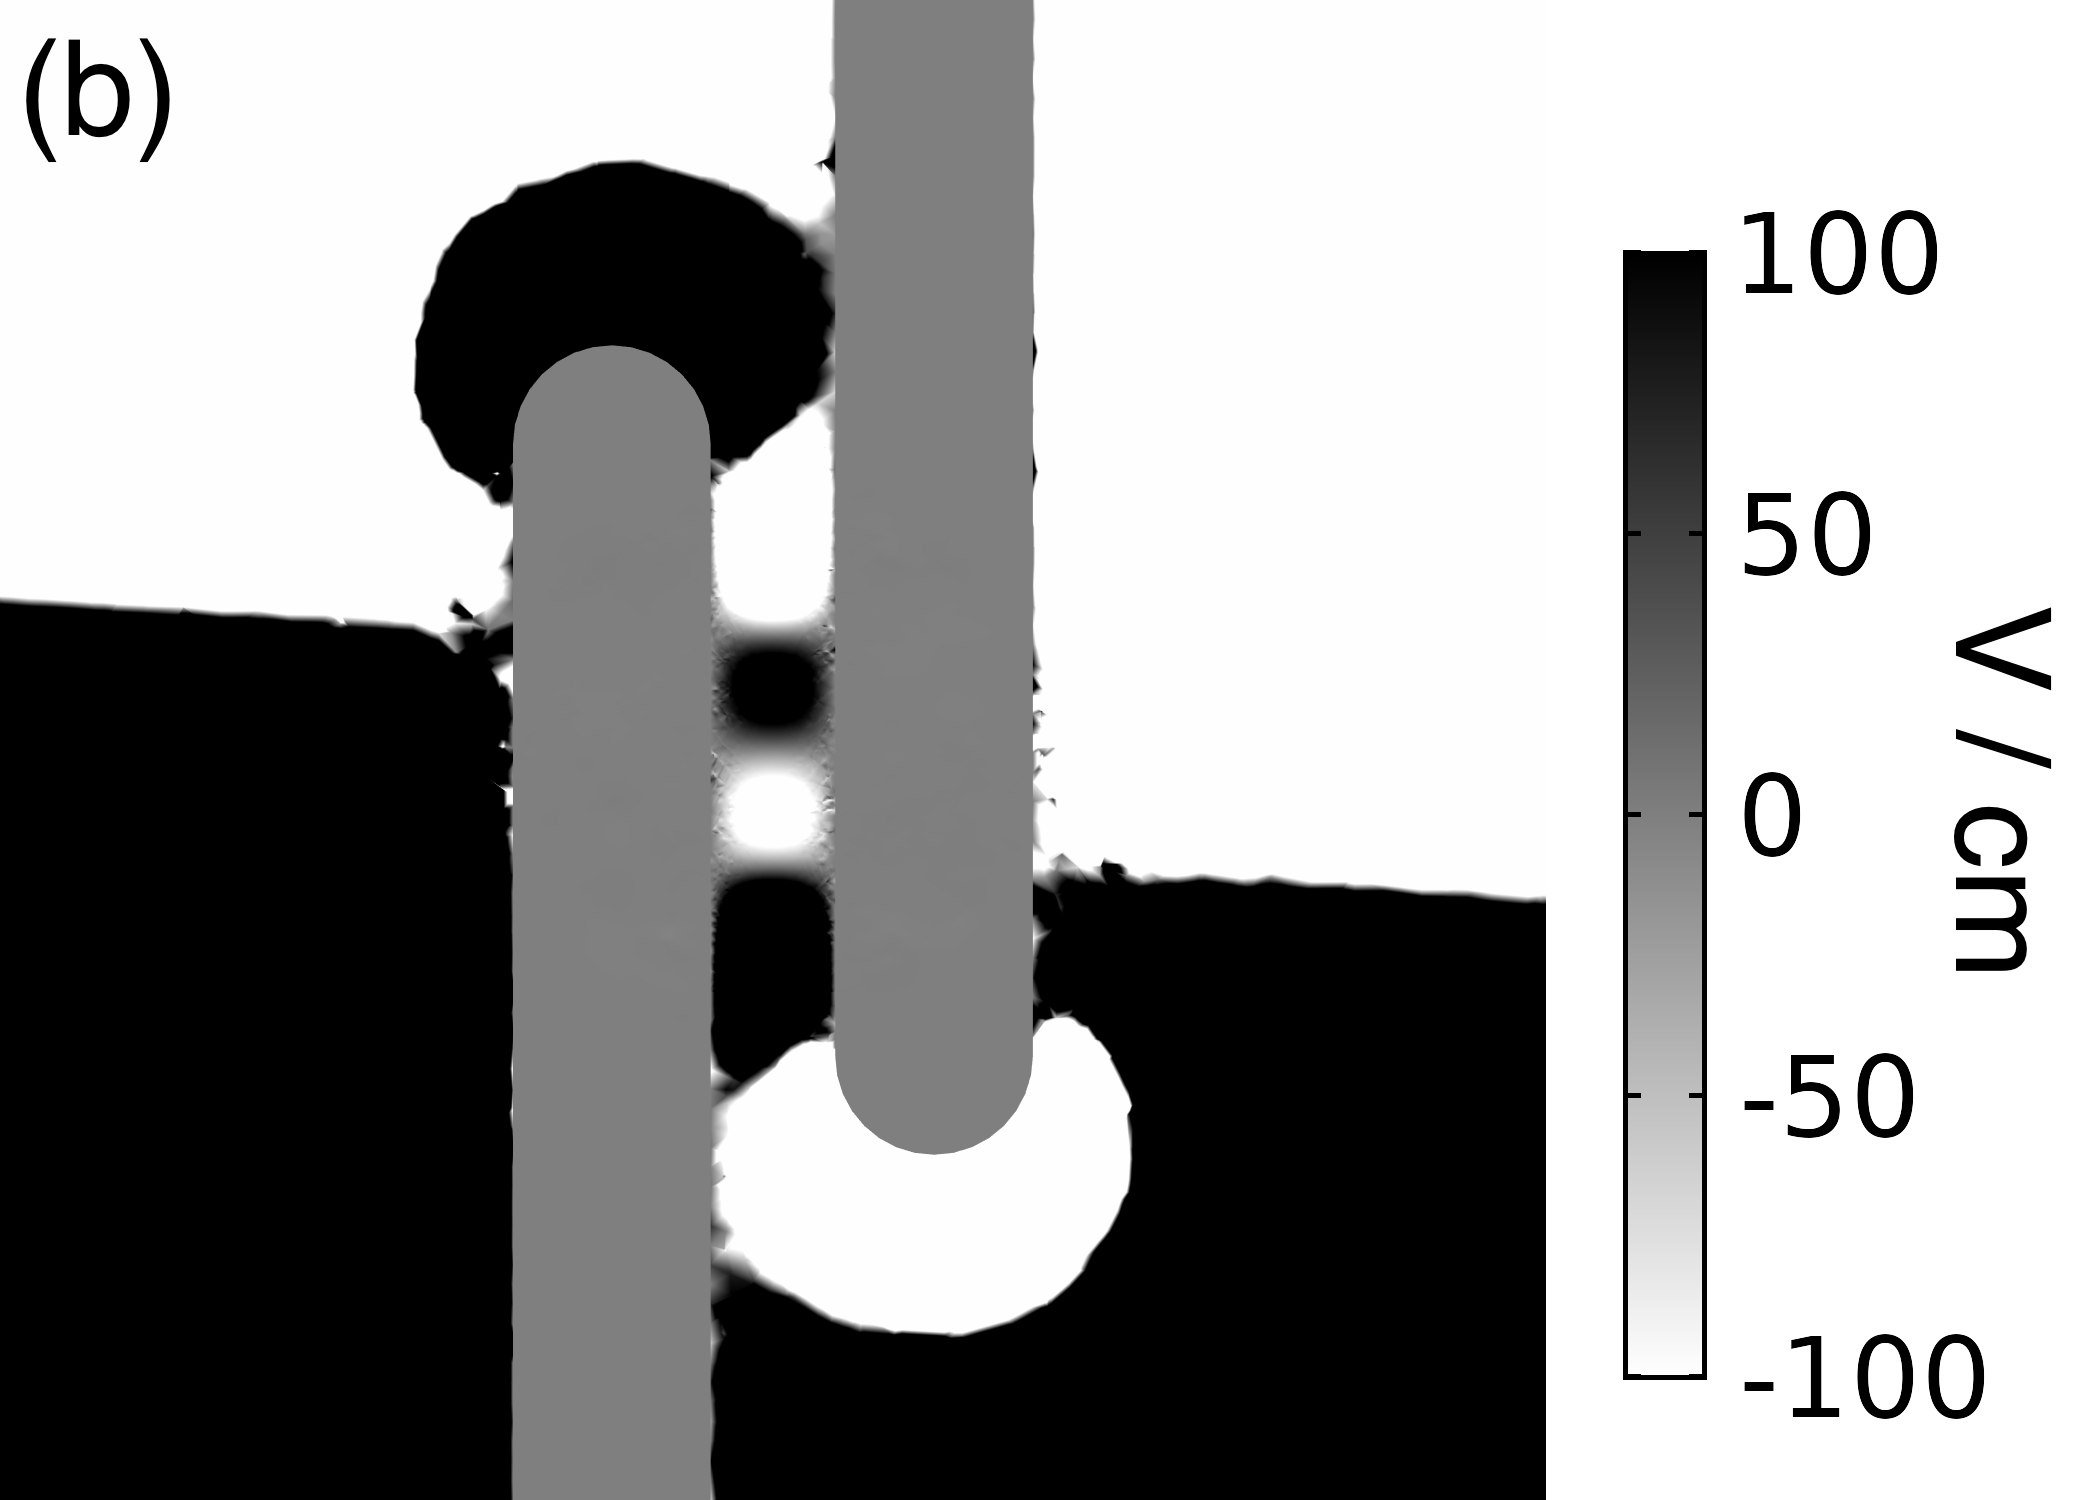
\includegraphics[width=8cm]{offset-avoid-loss-Ey.png}
\caption[Fields Close to Zeros of SF Mode]{\label{offsetavoid}
(a) Electric field magnitude in the transverse plane bisecting a pair of pins. A line of near-zero field is evident.
(b) The $\hat{y}$ component of the Electric field vector, where $\hat{y}$ is upwards, the direction which breaks the 2D symmetry and lifts the line of Electric field zero. The checker-like structure close to the central axis shows that there is actually a 3D electric quadrupole, with very slight restoring force in the vertical direction. This is relevant to reducing non-adiabatic transitions through intentional misalignment.
}
\end{figure}



\section{Decelerator Manufacturing}

Beginning in Fall of 2015, an effort was undertaken to manufacture a new decelerator capable of slowing a beam generated with Neon as a buffer gas. 
This effort was begun in parallel with ordering of a new Even-Lavie pulsed valve~\cite{Even2015}, which boasts significant gains especially for lighter carrier gases\footnote{It is difficult to verify such a claim, which concerns the relative performance of different valves with different carrier gases. The claim of better performance for an Even-Lavie valve only with lighter carrier gases comes from verbal discussions with SYT van de Meerakker during his sabbatical at JILA in the winter of 2015-2016.}.
Initially Argon was considered, but foolish zeal on the part of the author led to Neon, although at least he was talked out of Helium.

\subsection{Modeling}

Simulations were used to determine the optimal length for the device, or at least a length that would slow OH beginning at Neon speeds without comparable performance to the previous generation, see Fig.~\ref{fig:mp_elength_phaseload}a.
It was determined that something closer to $350$ stages should be ideal for loading the magnetic pin trap at $\phi\sim 55^\circ$, and so a $333$ stage device was planned.
Sensitivity of decelerator performance to pin pair spacing was also studied, and found not to have a significant effect, see Fig.~\ref{fig:mp_elength_phaseload}b.
Thinking in terms of the effective trap, this reduction shrinks the spatial extent of the longitudinal trap, but increases the velocity extent of the transverse traps, since the transverse focusing becomes more frequent.
The spacing was reduced from $5.461$~mm in the previous generation to an even $5$~mm.

\begin{figure}[t!]
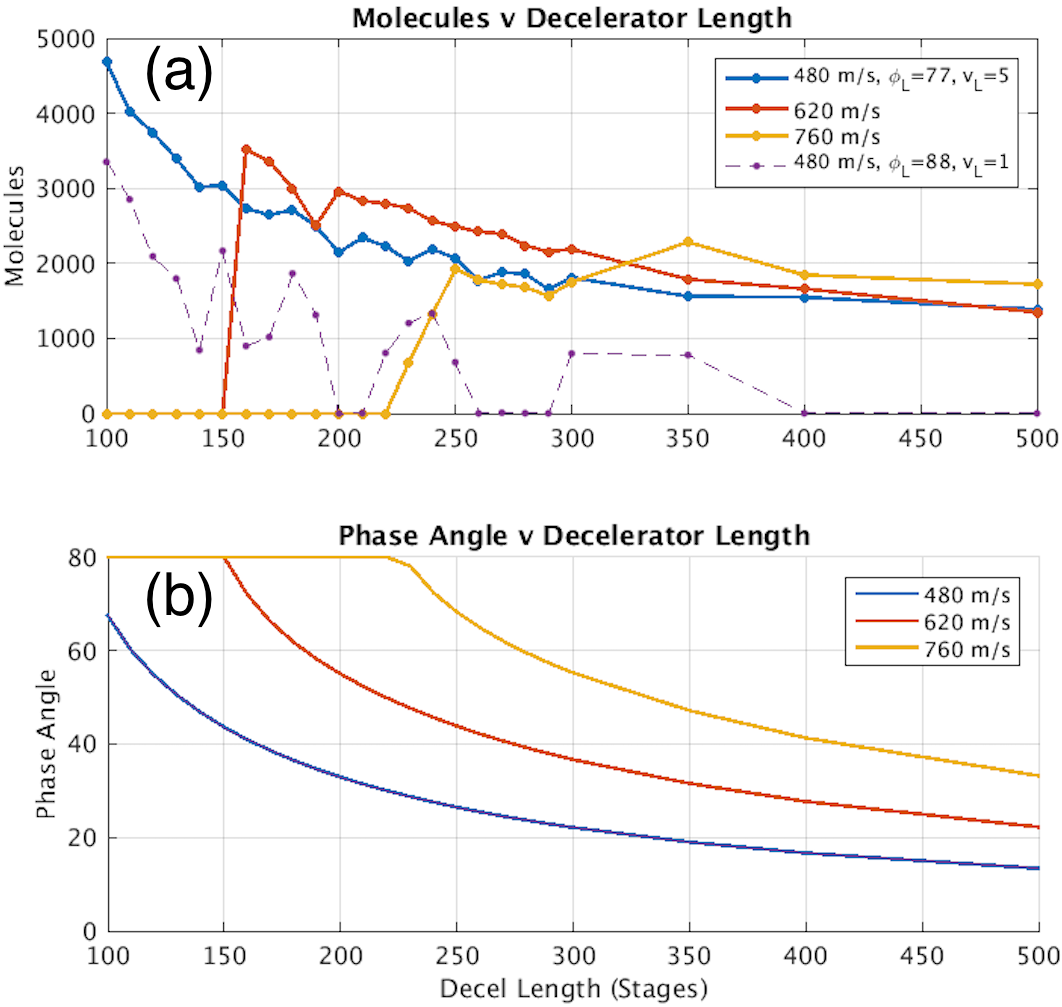
\includegraphics[width=9cm]{Slowing/mp_elength_phaseload.png}
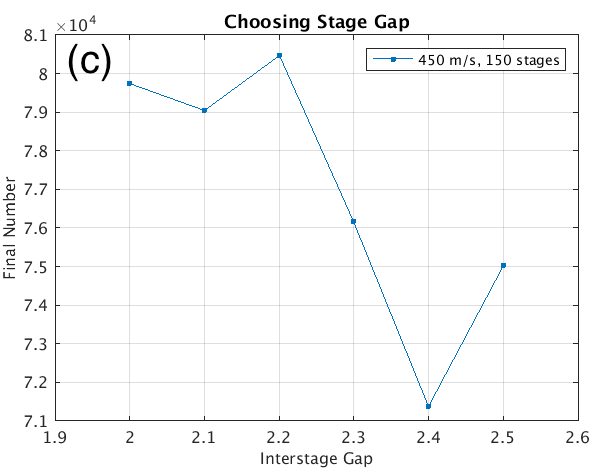
\includegraphics[width=7cm]{choosegap.png}
\caption[Decelerator Length Simulation]{\label{fig:mp_elength_phaseload}
Simulation results for deceleration and loading verses decelerator design parameters. (a) Loading efficiency is studied as a function of three initial speeds and various decelerator lengths. A ramping of the phase angle is used in the final few stages for further optimized loading. Increased length is observed not to facilitate improved trap population beyond some initial threshold value, likely due to the inefficiencies of the deceleration modes used at the time. (b) The selection of phase angle to achieve slowing to rest as a function of decelerator length is also shown. (c) The interstage gap is also studied.}
\end{figure}



\subsection{Mechanical Considerations}\label{sec:mechconsider}

In order to address manufacturing costs and installation time associated with such a long device (up from $142$ stages previously~\cite{Sawyer2007}, and $69$ before that~\cite{Bochinski2004}), we spent some time investigating the possibility of separate modules or of extensions mechanically affixed to the existing rods.
Ultimately it was decided that the challenges associated with getting such things right were not warranted by our length, and that it would be best to tackle everything with one long set of rods, mounted in a cage made of several stages, see Fig.~\ref{fig:decelmountingimages}.
One significant change that was developed out of a partnership with a local manufacturing company\footnote{\href{https://hirshprecisionproductsinc.com}{Hirsh Precision Products, INC}.} was to use locking tapers on both the pins and their mounting holes to fix them in place.
This halved manufacturing costs for the rods, and removed the need for setscrews, which created a serious galling hazard on the previous device and led to several near-disasters when re-polishing pins.
A special tool was developed for pressing the tapered pins into their holes, or removing them, without scratching any polished surfaces\footnote{The design is publicly available on \href{https://www.instructables.com/id/Scratch-Free-Press-Tool/}{Instructables}}.
We had also run into high voltage issues when using $MoS_2$ powder dissolved in isopropyl alcohol as a lubricating agent for said setscrews.
A key downside of the tapers was that they ended up creating a large sensitivity of final installed pin length on pin polishing procedure, since an extra unit thickness removed from the outside of the tapered pin causes the pin to sit $48$ units deeper into its hole (since the standard taper rate for tapered pins is a quarter inch per foot).
Fortunately this dimension is not critical for a pin-style Stark decelerator.
An additional challenge is that installation of many tapered pins acts as a fairly effective wedge for causing the main rod to bend ever so slightly.
After installation, we worked very hard to adjust the mounting structure so as to force the decelerator into proper alignment.
Lacking all requisite degrees of freedom, we settled for a precision tuning of the pin pair spacing, in the hope that as long as that remained correct, the molecules would be able to follow any slight bends in the device.
Finding a way to work with a larger diameter rod may have been preferable.
The tapered pins may be a good choice for other designs, especially if a vendor is used who can offer both surface quality and tolerancing at the same time\footnote{We worked with \href{http://www.tri-gon.com}{TriGON Precision} for polish after having Hirsh Precision Products INC manufacture the pins. They often expressed their preference to have manufactured the pins themselves in the first place, since we were asking them to get a high quality polish without removing too much material.}.

\begin{figure}[t!]
\centering
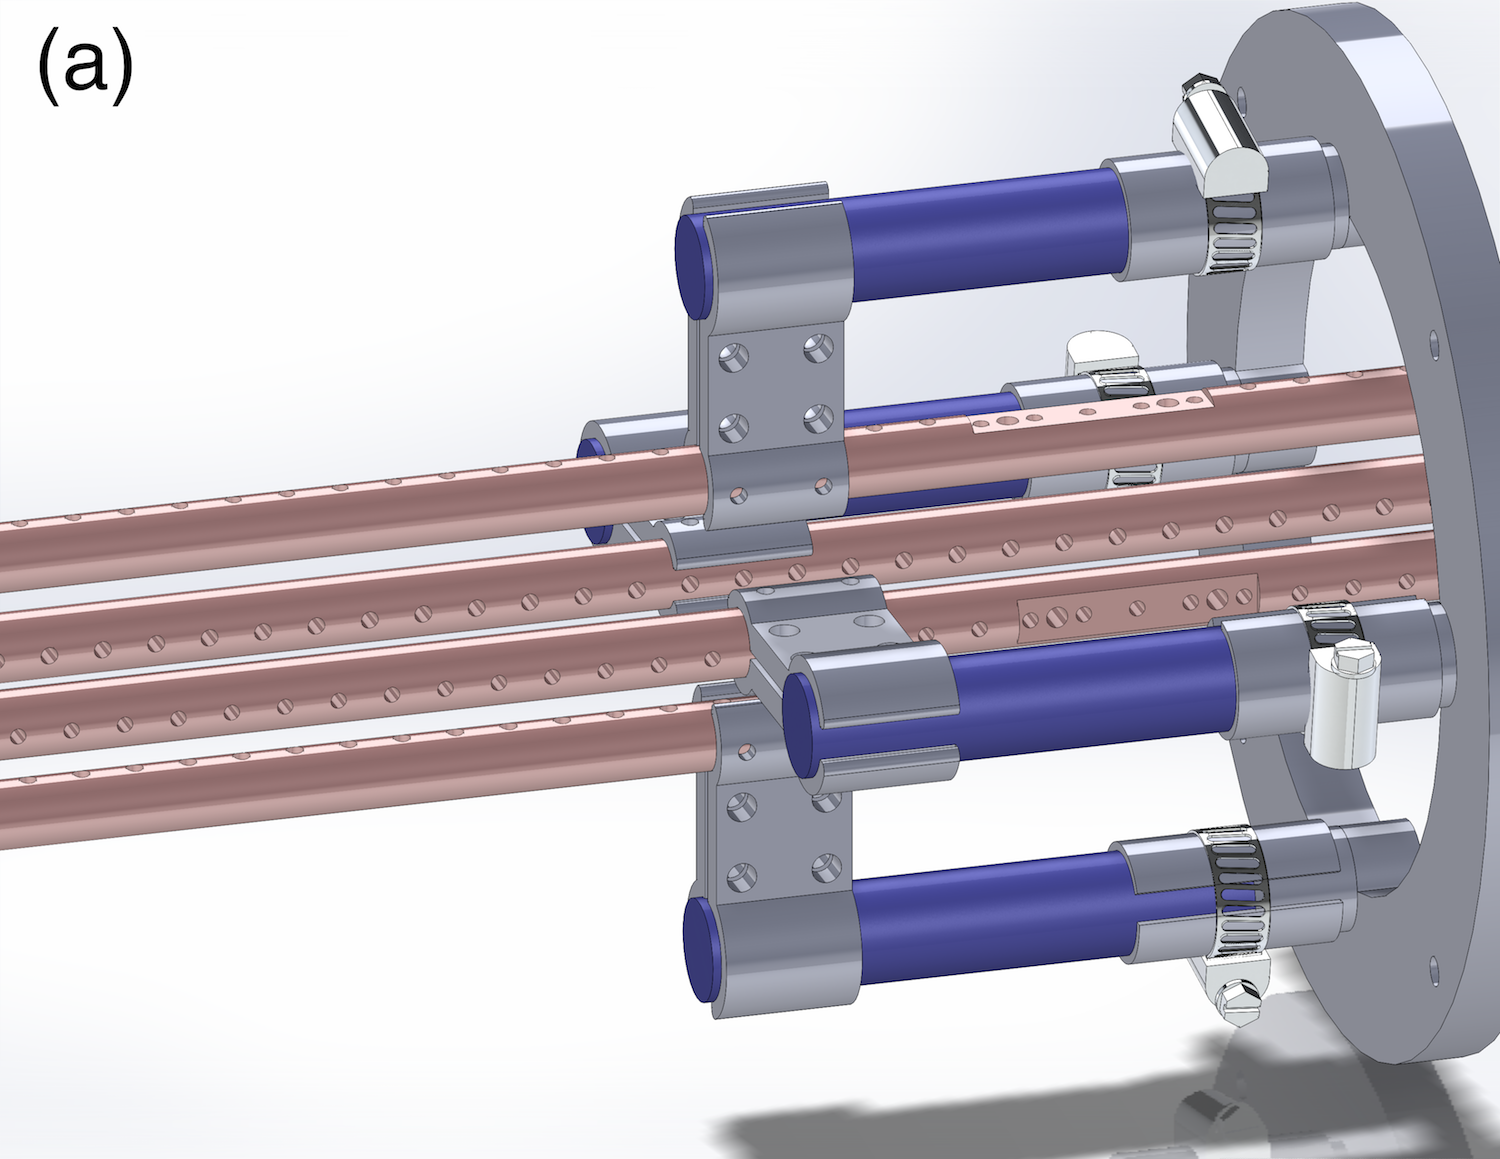
\includegraphics[width=8cm]{Slowing/MountingCageSystem1.png}
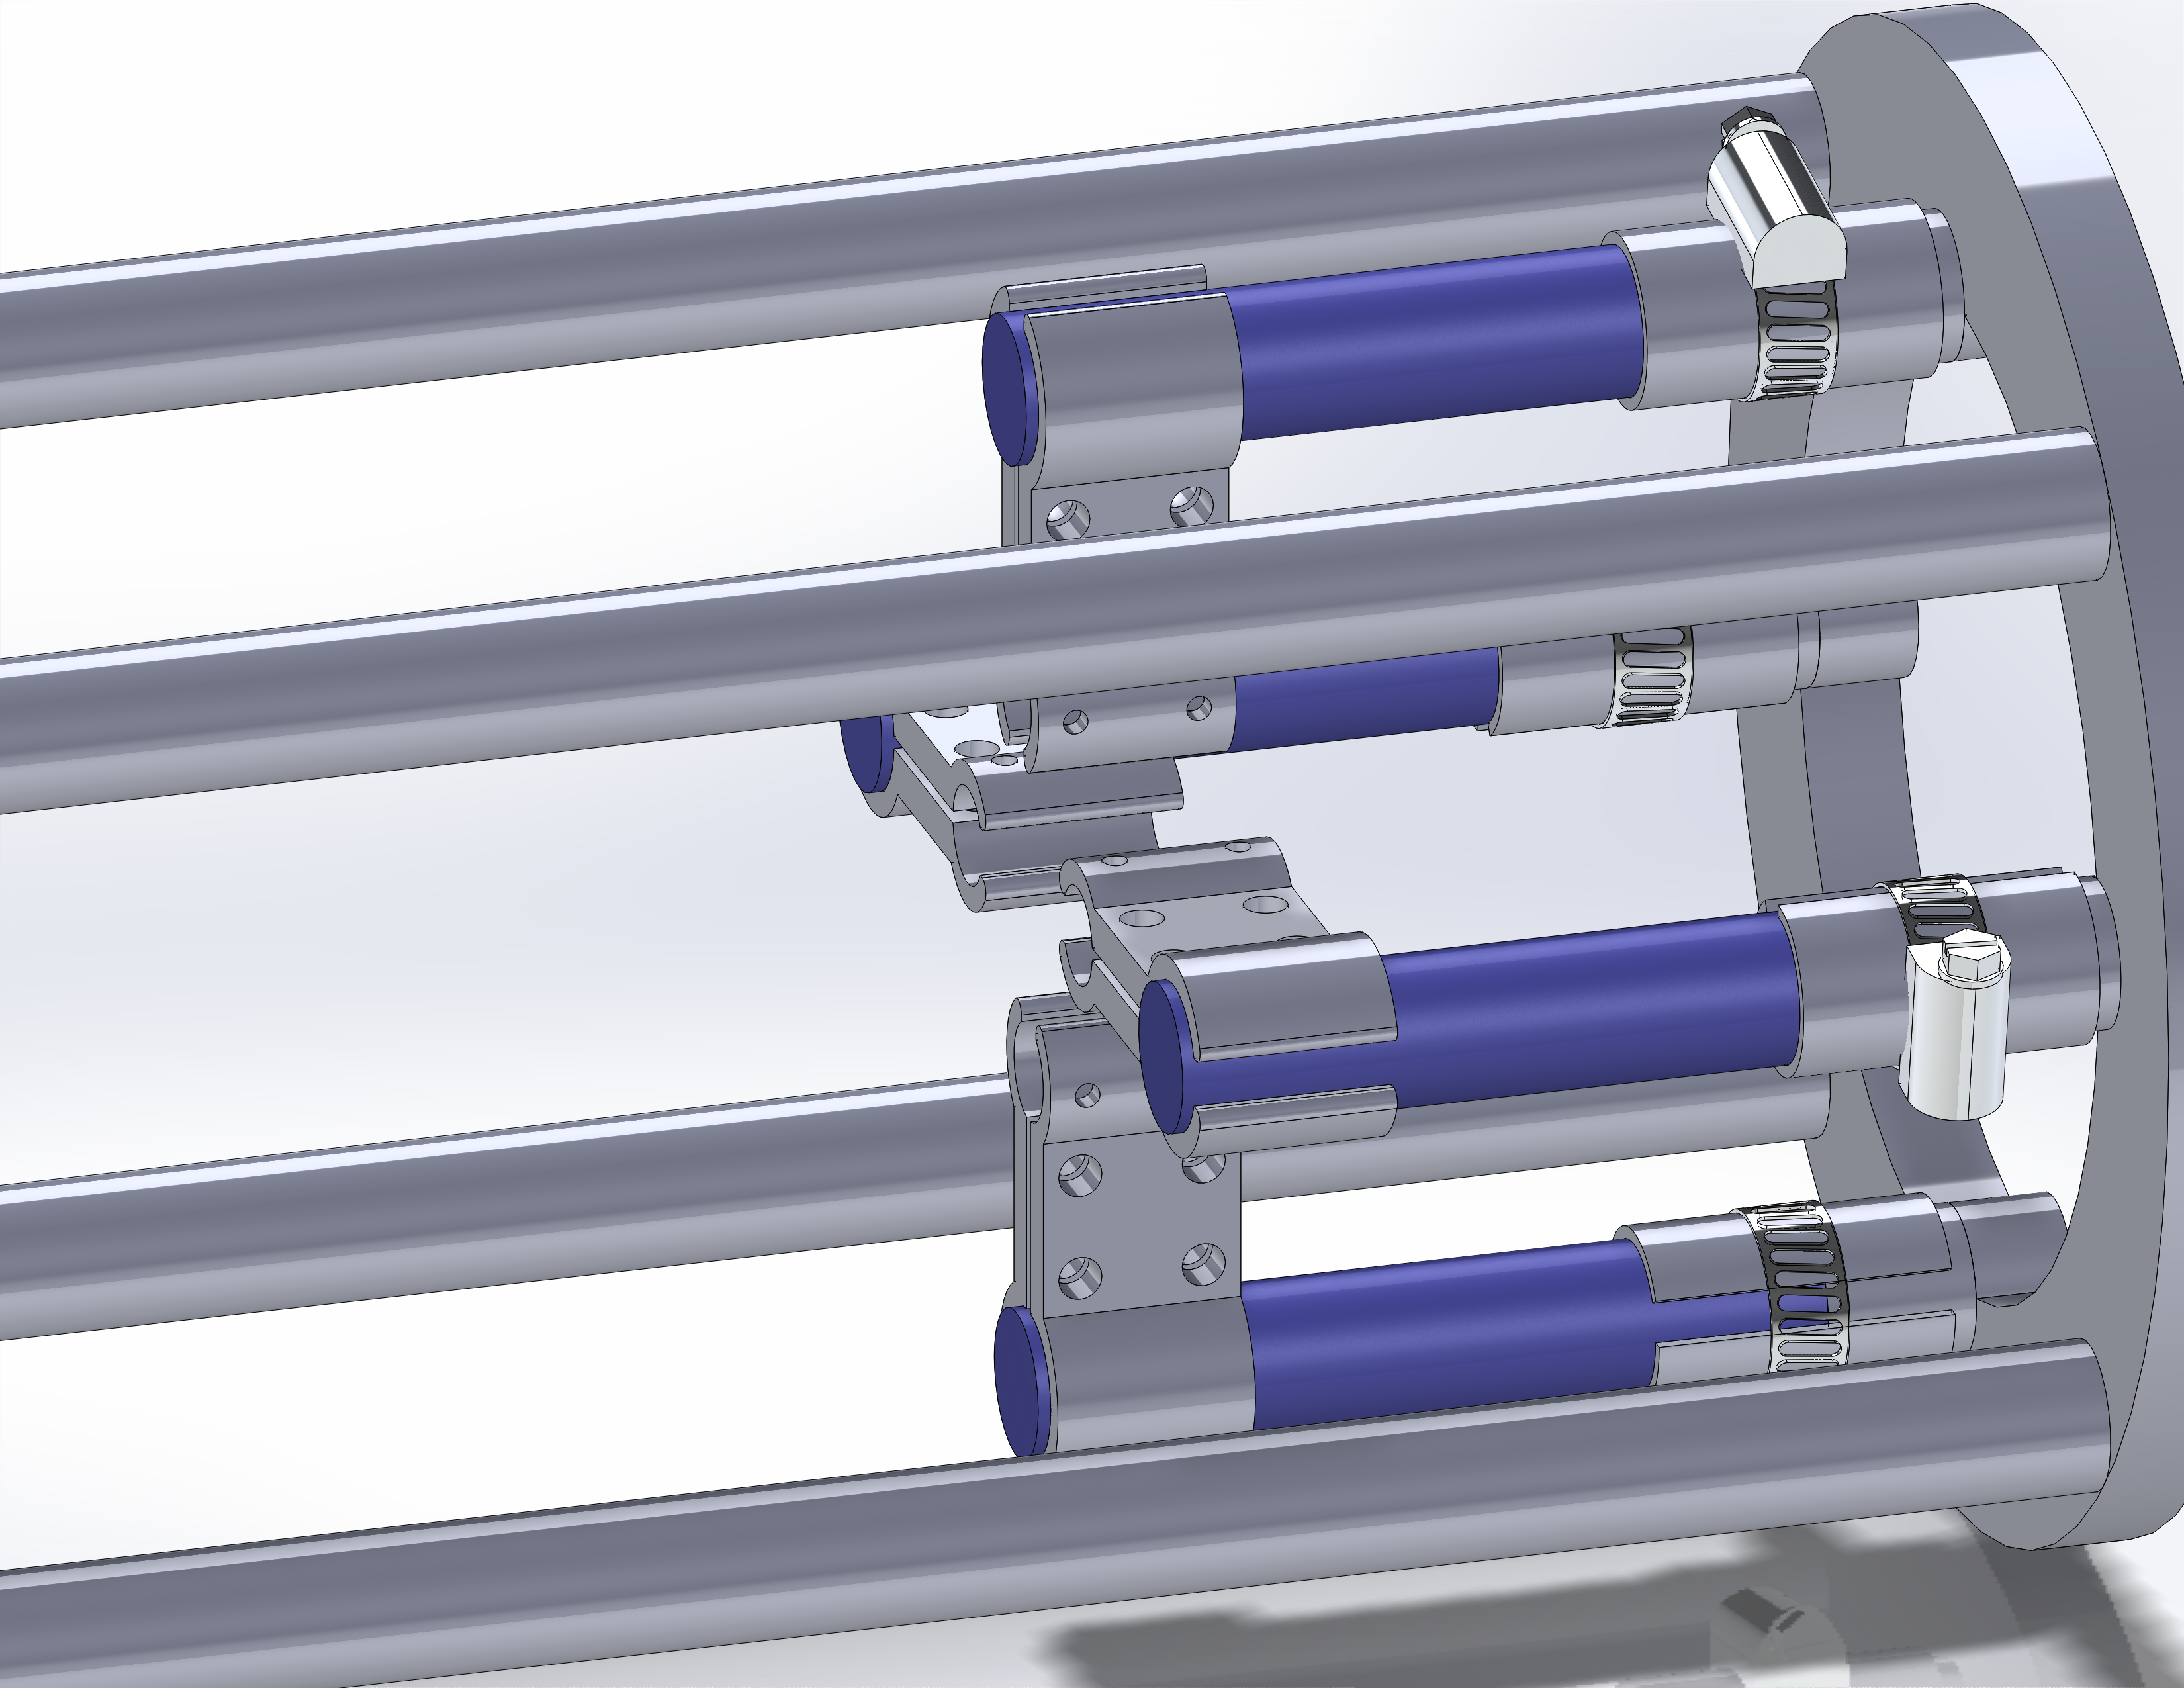
\includegraphics[width=8cm]{Slowing/MountingCageSystem2.png}\\
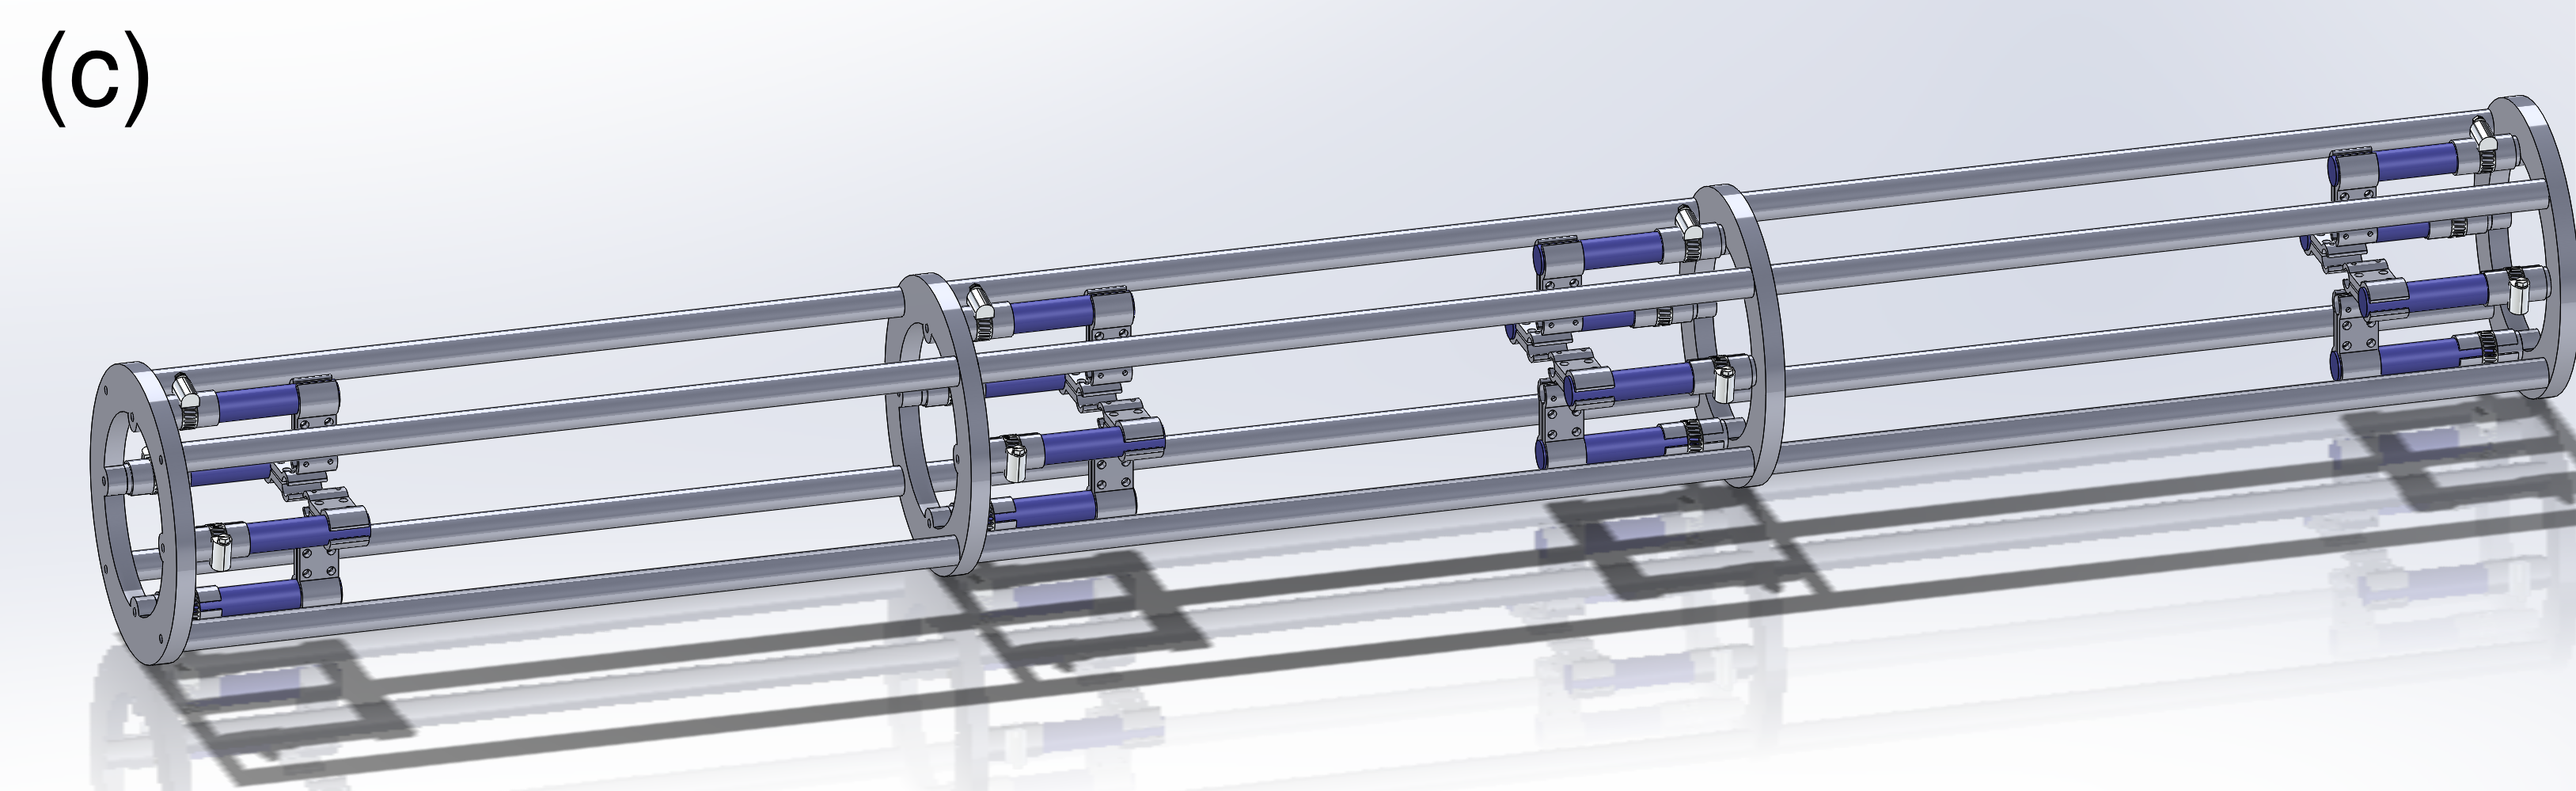
\includegraphics[width=\linewidth]{Slowing/MountingCageSystem3.png}
\caption[Decelerator Mounting Structure]{\label{fig:decelmountingimages}
Mounting structure of third generation Stark decelerator. Note large safety high voltage surface distance along glass rods, blue. (a). Clamping pieces grab on to the actual decelerator rods. A mounting flat, a vestige of an earlier design, is visible on the decelerator rod. (b) Decelerator rods hidden, cage connection rods shown. (c) Full view of the cage structure.}
\end{figure}


It is worth setting out a figure of merit to describe the extent to which such slight bends would be acceptable. 
For velocity $v$, a bend radius $r$ causes an acceleration $a=v^2/r$. 
For a given operation mode, we can characterize the transverse trap as a harmonic potential $U=\frac{1}{2}m\omega^2x^2$. 
In the case of a bent decelerator, this potential is a non-inertial frame, and the bending acceleration can be included as a fictitious force which causes the molecules to shift off of center in the trap.
The magnitude of this shift is given by the $x_s$ which satisfies:
\begin{equation}
\frac{\partial U}{\partial x}\biggr|_{x_s} = m_\text{OH}\frac{v^2}{r},
\end{equation}
from force balance. Solving:
\begin{equation}
x_s = \frac{v^2}{r\omega^2}.
\end{equation}
For SF mode, $\omega\sim1.0\text{ kHz}$, for F mode, $\omega\sim0.7\text{ kHz}$. Assuming that $x_s\sim0.2$~mm is acceptable, $10\%$ of the pin pair spacing, the allowed bend radius for $800$~m/s molecules is $3.2, 6.5$~km for SF, F modes.
Along the length of a $1.7$~m device, such bends amount to offsets of $1, 0.5$~mm.
Based on the observation that we are able to shine a laser beam all the way through the device, albeit without the expected $2$~mm square-like shape, bends in the device are unlikely to be significantly larger than these numbers, but likely on this order.

\subsection{High Voltage Arcing}

With the new design, an effort was made to address challenges that had developed with the mounting of the previous generation, which had been facilitated by MACOR, a machinable glass ceramic material.
The MACOR was found to allow surface currents, which also were un-phased by the surface path-length extension grooves that had been added to reduce their likelihood, as can be seen in Fig.~\ref{macorbad}.
There was never a clear indication that these surface arcs were actually causing a reduction in molecule yield, but nevertheless it seemed wise to make an attempt at improving the situation.
In reviewing literature~\cite[Sec.~4.3.3]{Faircloth2013} and consulting other opinions, it was found that the previous geometry did not respect recommended considerations regarding so-called ``triple-points'' where vacuum, dielectric, and conductor meet. 
These are advised to be recessed or otherwise manipulated so as to minimize the electric field at their location~\cite{Miller1989}.
This is achieved in the new design, as well as increasing the safety distance and removing reliance on sharp insulator features, by the geometry visible in Fig.~\ref{fig:decelmountingimages} and heavily influenced by~\citep[Fig.~4]{VanDeMeerakker2006}.
Borosilicate glass rods were selected for their vacuum and insulating properties, with alumina rods as a close second.


\begin{figure}[t!]
\centering
\vspace{1mm}
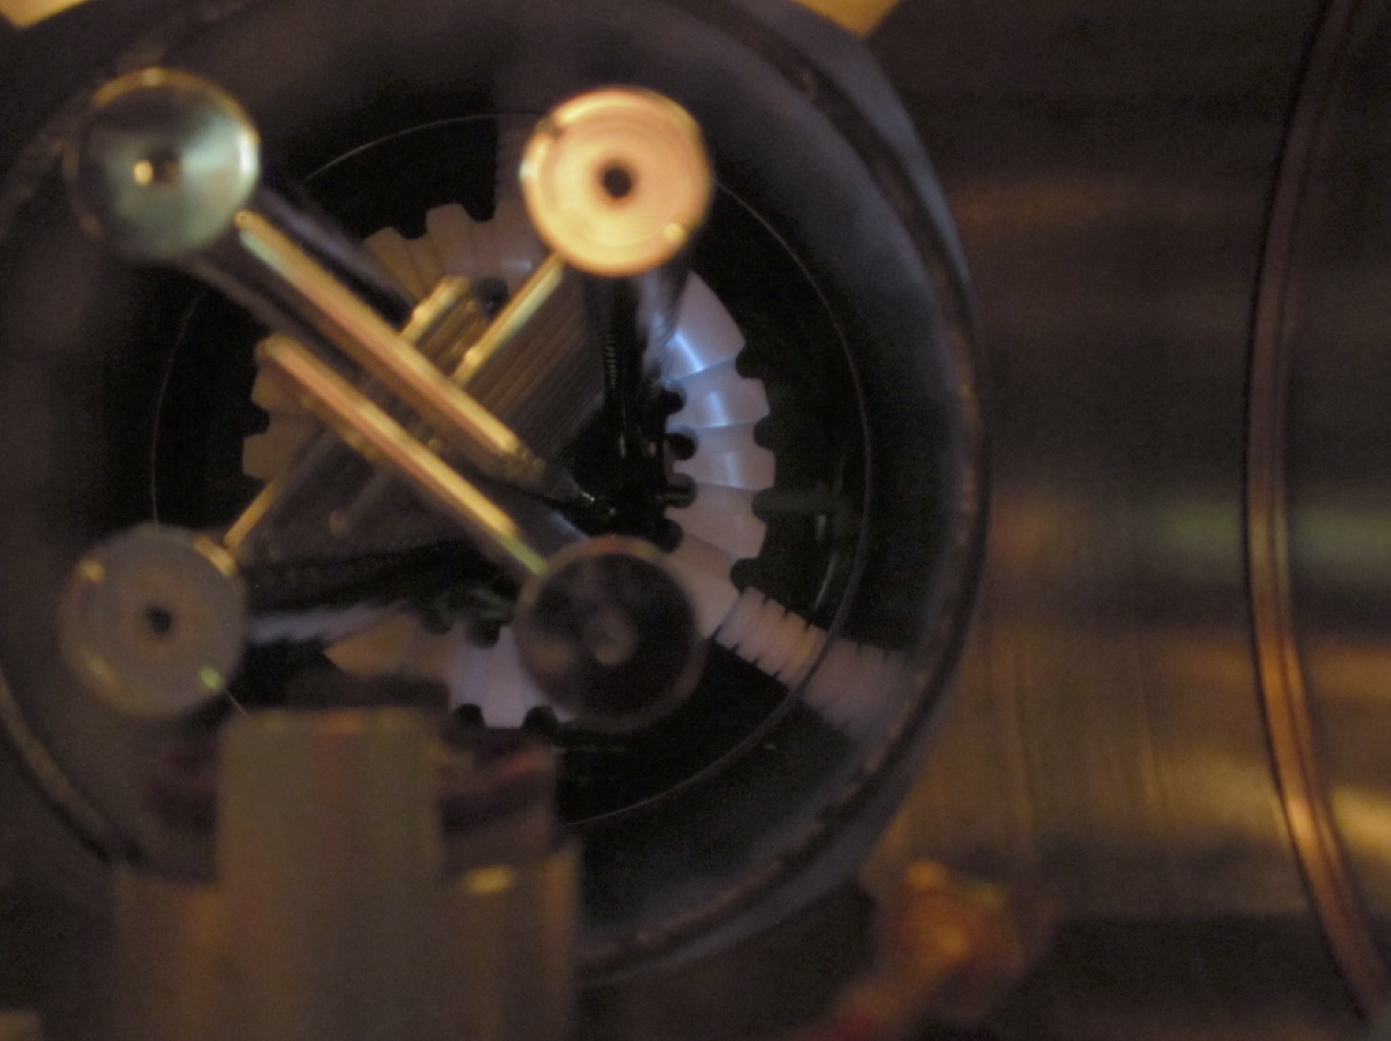
\includegraphics[width=9cm]{Macor2.png}
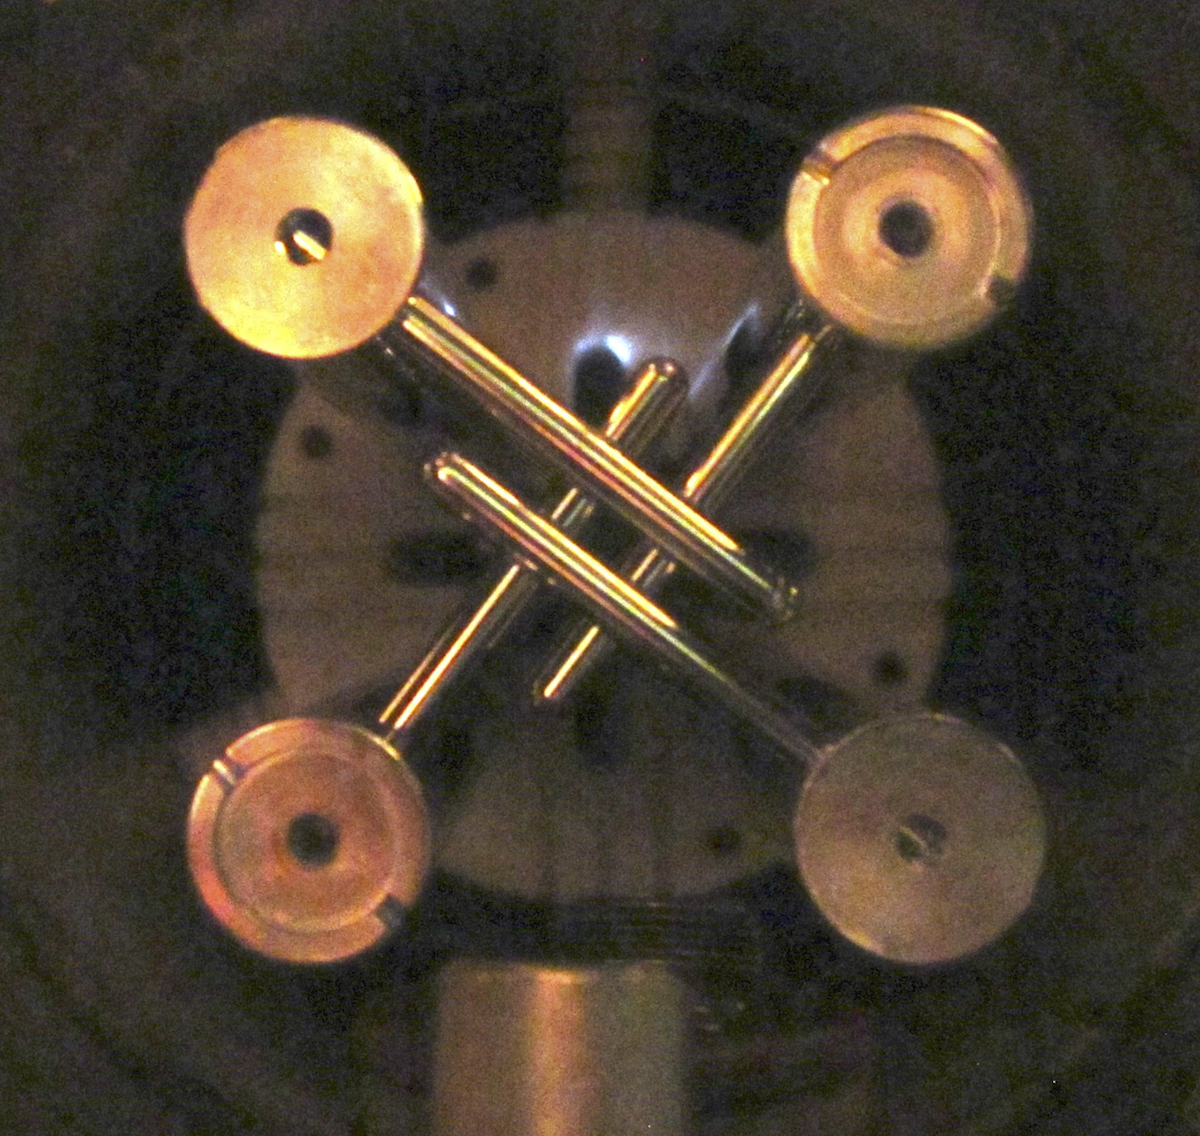
\includegraphics[width=7.11cm]{Macor1.png}
\caption[MACOR Surface Arcs]{\label{macorbad}
MACOR surface arcs. At left, arcing on an insulator original to the manufacture of the second generation device~\cite{Sawyer2007}. At right, arcing on a redesigned version, undertaken concurrently with a re-polishing of the last twenty decelerator pins performed in the fall of 2014. Here it is evident that the path-length extension grooves are not helpful.}
\end{figure}

\subsection{High Voltage Electronics}

In the design of the new decelerator, the capacitive load presented by the decelerator was an important consideration.
For a long enough device, it would in principle become necessary to purchase a new set of switches capable of providing higher currents.
Fortunately, prior to the design effort which culminated in the third generation decelerator system, it was realized that the capacitance of the cables connecting the high voltage switches to the decelerator actually dominated the capacitance seen by the switches.
It was thus possible to operate the original electronics with the new decelerator at even lower load than previously, thanks to a systematic effort of relocating electronics so as to minimize all high voltage cabling, especially between the transistor switches and the decelerator rods.
Considerable influence in the design and execution of this effort was taken from~\citep[Fig.~4.6]{Scharfenberg2012}.

An even more significant challenge constitutes the management of multiple output states as required for the realization of the SF and VSF modes discussed above. 
Such an effort was successfully undertaken in the operation of certain traps discussed later in this thesis, but only at very low repetition rate.
In considering circuitry involving the use of multiple transistor switches arranged in series or parallel it is essential that all parasitic elements of the devices are taken into account, especially the parasitic capacitances in parallel with the drain and source terminals, which can form the dominant current load as seen by other transistor switches in the circuit.
At the time of this writing, careful collaboration with engineers at Behlke GMBH resulted in the selection of a device\footnote{Behlke HTS-301-151-SiC, options HFB, ILC, ALL-OFF-BIPOLAR.} that should be capable of operating SF mode, and VSF if a second such device is ordered. 
The device has yet to arrive after requiring a rebuild following a miscommunication pertaining to the specification of options for the switch.

\subsection{Capacitance Matrix\label{capmatsection}}

It is also relevant to again consider the capacitive load associated with switching between various distinct field distributions.
In this case, it becomes necessary to treat the full system of electrodes not as a single capacitor but actually as a network of different capacitors most efficiently captured in the form of a capacitance matrix $C_{ij}$ satisfying:
\begin{equation}
Q_i = C_{ij}V_j,
\end{equation}
so that a vector of charges on each conductor can be obtained given a vector of voltages on each.
Surprisingly, in our system the capacitance between a pair of rods with parallel pins is actually slightly less than that between a pair of rods whose pins are orthogonal, see the matrices reported in Fig.~\ref{capmat}.
An important corollary of the multi-capacitor system is that the transient dynamics of the system do not follow the usual RC behavior, as shown in panel (c) of Fig.~\ref{capmat}.

\begin{figure}[t!]
\centering
\includegraphics[width=\linewidth]{capmats.png}
\caption[Capacitance Matrix for Third Generation Decelerator]{\label{capmat}
Capacitance matrices from LRC meter and simulation for third generation decelerator. (a) Capacitance matrix by measurement and (b) by COMSOL simulation. (c) Example of the multi-timescale dynamics that can occur when solving the transient response of a capacitive system to sudden changes in the voltages applied to the electrodes.
}
\end{figure}

\subsection{Differential Pumping}

One key downside of Stark decelerators compared to conventional alkali Zeeman slowers is the lack of feasible differential pumping schemes.
This challenge stems from the difficulty of mounting anything close to the Stark decelerator without violating high voltage safety on some level.
Electric fields also interact more strongly with most materials compared with electric fields, and so there is no tube like structure that could be mounted inside the pairs of decelerator pin without shunting away most of the field lines, not to mention surface arcing.
Nonetheless, in the third generation of the experiment a technique was developed for differentially pumping the end region of the Stark decelerator from the other vacuum regions, using a glass baffle structure which comes close to the decelerator on all sides but without making any surface contact, see Fig.~\ref{glassbaffleimage}.

\begin{figure}[t!]
\centering
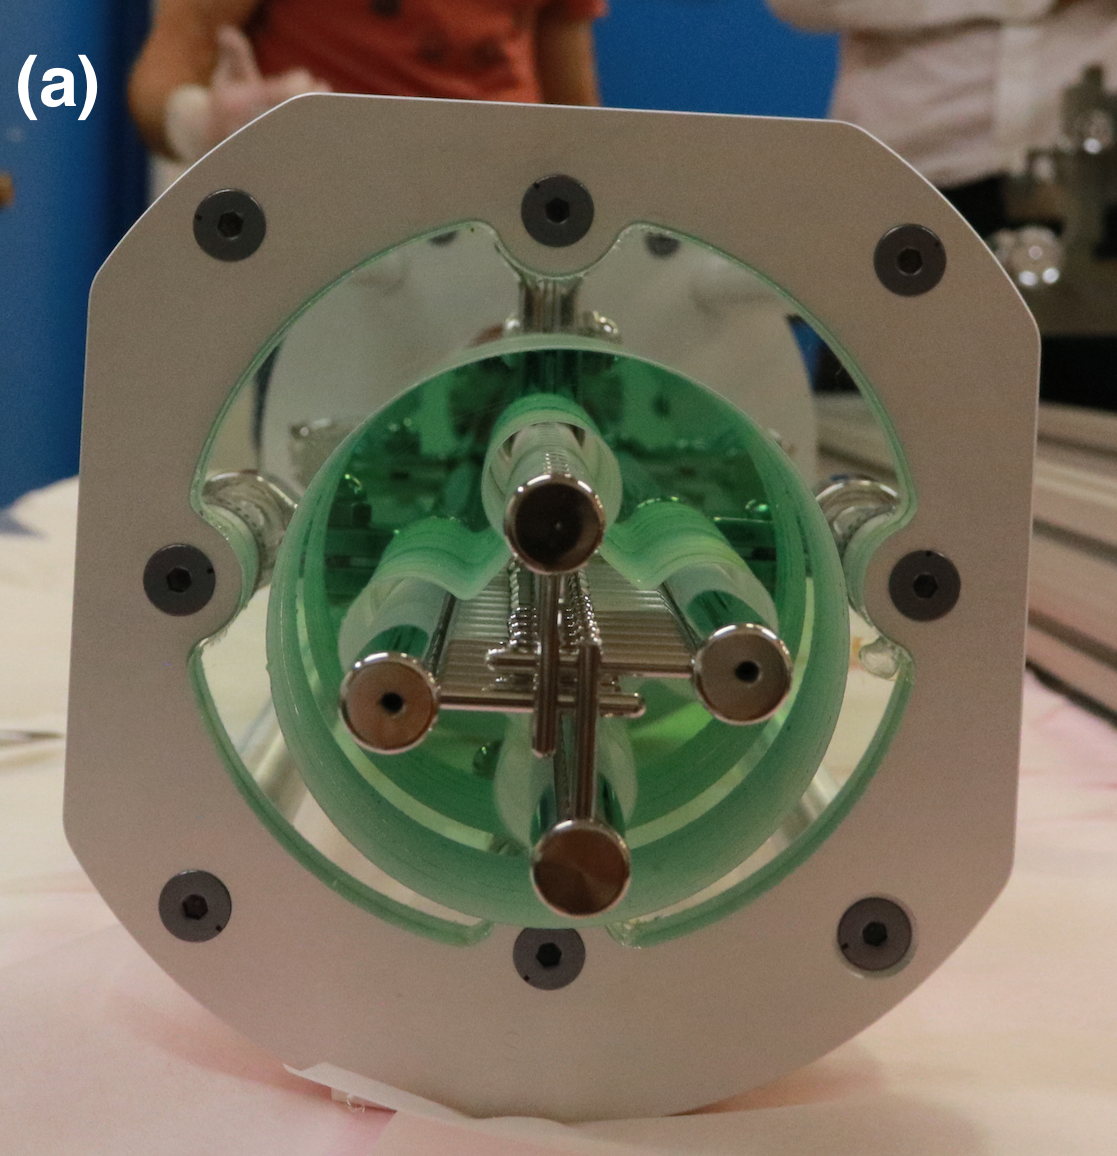
\includegraphics[width=6cm]{Glass-Baffle-Headon.png}
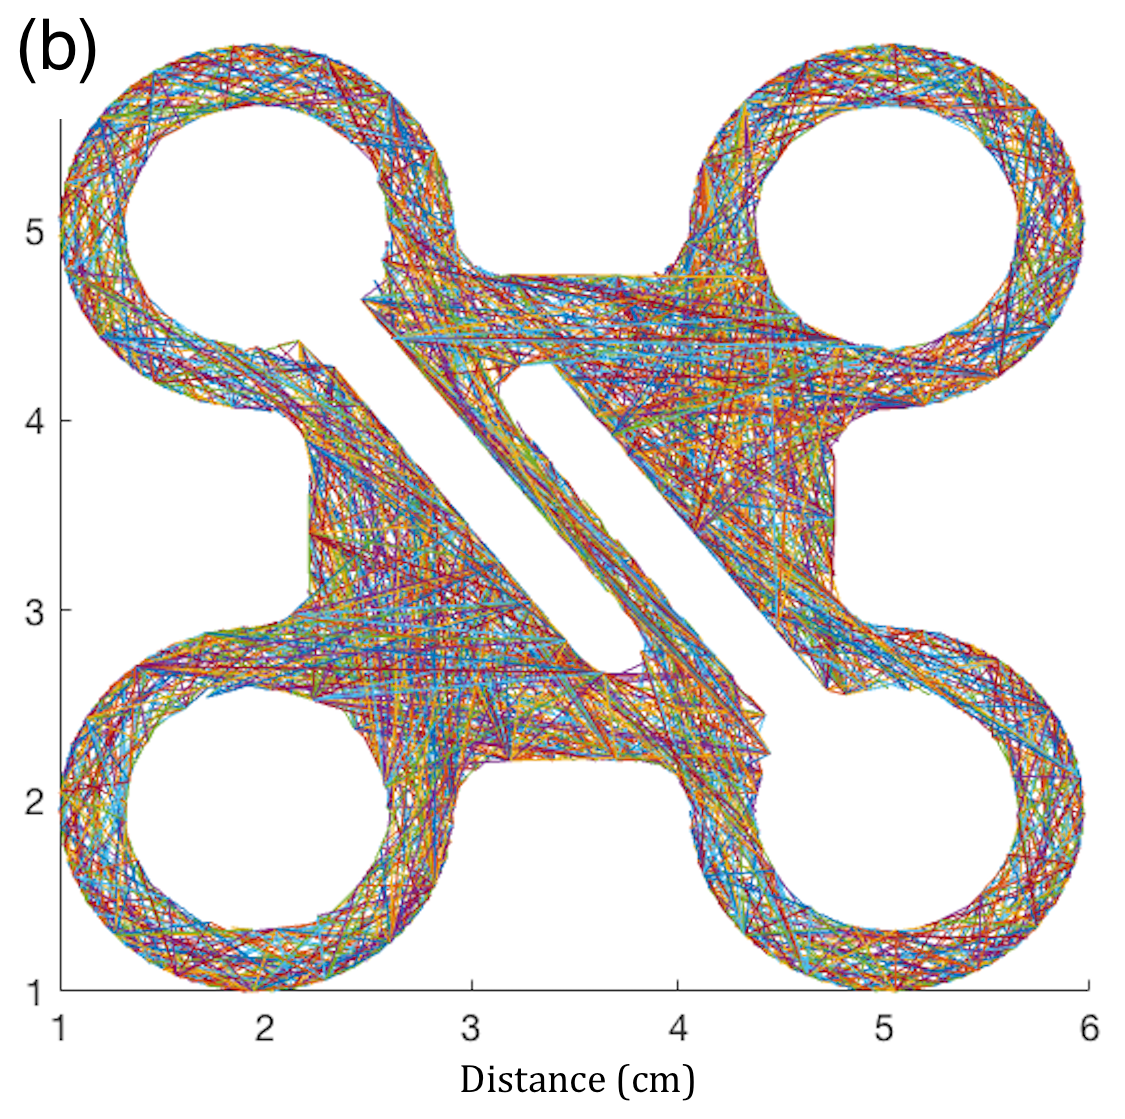
\includegraphics[width=6cm]{SampleChordFilling.png}\\
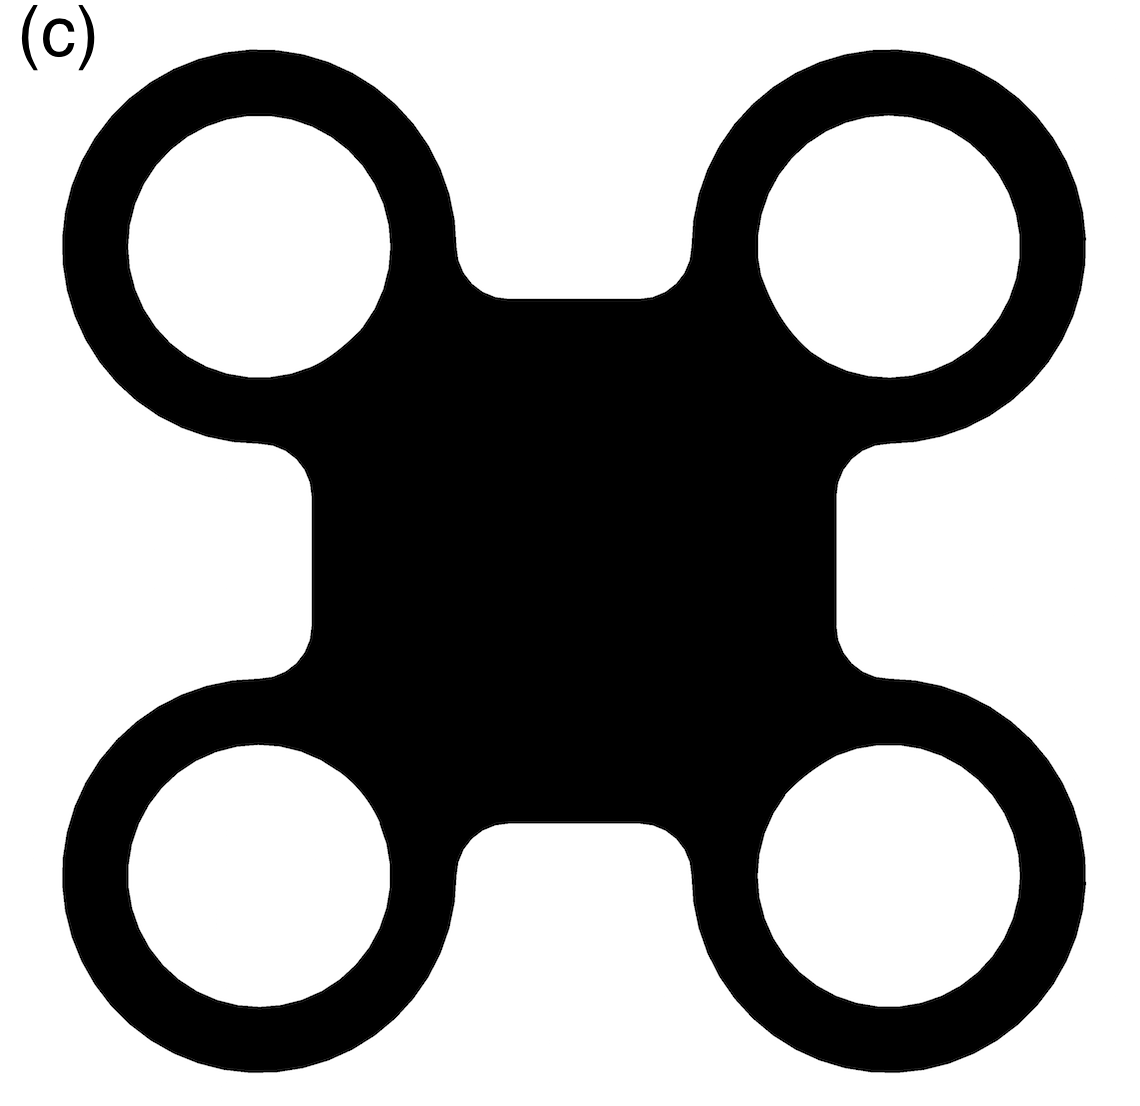
\includegraphics[width=6cm]{decel_conductance_0.png}
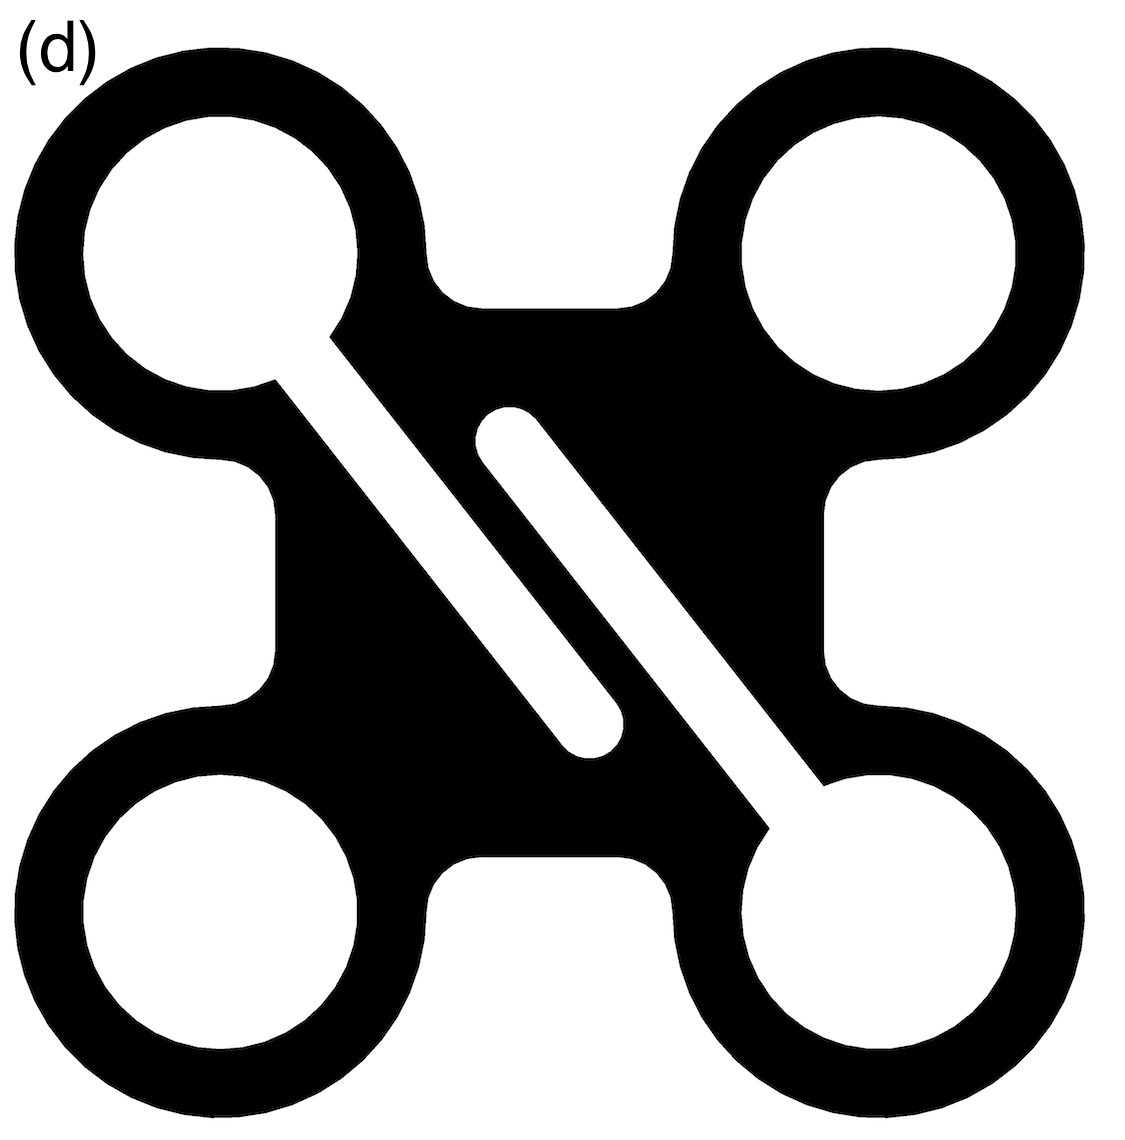
\includegraphics[width=5.7cm]{decel_conductance_2.png}
\caption[Glass Baffle for Differential Pumping]{\label{glassbaffleimage}
Glass baffle for differential pumping. Conductance of about $20$~L/s for Neon. (a) Manufactured from a stack of water-jetted glass slabs, glued together with a low outgassing epoxy. (b) Sample output from pipeConductance.m, a conductance calculation package developed for this application\footnotemark. One tenth of the chords used for calculation are shown. Calculation is well converged as far as chord inclusion is concerned. (c,d) Profiles used for specifying cross sections for conductance calculation. Conductance is $24.2$~L/s for (c), $12.7$~L/s for (d).}
\end{figure}

\footnotetext{\label{pipefootnote}See the \href{https://www.mathworks.com/matlabcentral/fileexchange/60748-dreens-pipe-conductance}{MATLAB file exchange} or my \href{https://github.com/dreens/pipe-conductance}{Github page}.}
I devoted some effort to determining the vacuum conductance of the unusual cross section one obtains by mounting something close to the outside of a Stark decelerator.
While commercial software exists for determining conductances and pump-down times for arbitrary geometries, these options would require very high mesh densities and very long computation times given the small scale and detail of the geometry.
A better option is to work in two dimensions where general expressions amenable to numerical integration exist~\citep[Eq.~14]{Steckelmacher1966}.
Of course the decelerator is not quite translationally invariant in the molecular direction, because the pins are discontinuous.
A worst case can be had by assuming no pins installed, and comparing this to the case of only two or four rows of pins being installed, see panels (c) and (d) of Fig.~\ref{glassbaffleimage}.
My conductance calculations are nicely packaged and publicly available$^{\text{\ref{pipefootnote}}}$.
Conductance would be $24.2$~L/s without any pins, $12.7$~L/s with two solid rows of pins, and $8.6$~L/s with four solid pin rows.
Given our $500$~L/s pumping speed in the chamber downstream of the baffle, the baffle therefore affords something like a twenty-fold differential pressure reduction in the gas load coming through the baffle from the beam source.
This could be measured somewhat easily using a leak valve, but we have simply never bothered.
Excellent suppression of Neon is observed, with an RGA mounted in the trap chamber not even detecting whether or not the pulsed valve is turned on, at least with a skimmer in place in the source chamber.
%During some of our tests of decelerator clogging effects, the skimmer was actually removed, in which case Neon could be detected by the RGA.


\ifx\justbeingincluded\undefined
\bibliographystyle{unsrtDR}	% or "siam", or "alpha", etc.
\bibliography{allrefs}		% Bib database in "allrefs.bib"
\end{document}
\fi
